%%% Hlavní soubor. Zde se definují základní parametry a odkazuje se na ostatní části. %%%

%% Verze pro jednostranný tisk:
% Okraje: levý 40mm, pravý 25mm, horní a dolní 25mm
% (ale pozor, LaTeX si sám přidává 1in)
\documentclass[12pt,a4paper]{report}
\setlength\textwidth{145mm}
\setlength\textheight{247mm}
\setlength\oddsidemargin{15mm}
\setlength\evensidemargin{15mm}
\setlength\topmargin{0mm}
\setlength\headsep{0mm}
\setlength\headheight{0mm}
% \openright zařídí, aby následující text začínal na pravé straně knihy
\let\openright=\clearpage

% číslované subsubsection
\setcounter{secnumdepth}{3}
\setcounter{tocdepth}{3}

%% Pokud tiskneme oboustranně:
% \documentclass[12pt,a4paper,twoside,openright]{report}
% \setlength\textwidth{145mm}
% \setlength\textheight{247mm}
% \setlength\oddsidemargin{15mm}
% \setlength\evensidemargin{0mm}
% \setlength\topmargin{0mm}
% \setlength\headsep{0mm}
% \setlength\headheight{0mm}
% \let\openright=\cleardoublepage

%% Pokud používáte csLaTeX (doporučeno):
\usepackage{czech}
%% Pokud nikoliv:
%\usepackage[czech]{babel}
%\usepackage[T1]{fontenc}

%% Použité kódování znaků: obvykle latin2, cp1250 nebo utf8:
\usepackage[utf8]{inputenc}

%% Ostatní balíčky
\usepackage{graphicx}
\usepackage{amsthm}
\usepackage{amsmath}
\usepackage{color}
\usepackage{colortbl}
\usepackage[bottom]{footmisc}
\usepackage{multirow}
\usepackage{float}
\usepackage[font=scriptsize,labelfont=bf]{caption}

\definecolor{seda}{rgb}{0.7,0.7,0.7}
\newcommand{\argmax}[1]{\underset{#1}{\operatorname{arg}\,\operatorname{max}}\;}
\DeclareFontFamily{OT1}{pzc}{}
\DeclareFontShape{OT1}{pzc}{m}{it}{<-> s * [1.10] pzcmi7t}{}
\DeclareMathAlphabet{\mathpzc}{OT1}{pzc}{m}{it}

\usepackage[usenames,dvipsnames]{xcolor}



%% Zrušení odsazení odstavců
\usepackage{indentfirst}
\setlength{\parindent}{0em}
\setlength\parskip{2mm}

%% Balíček hyperref, kterým jdou vyrábět klikací odkazy v PDF,
%% ale hlavně ho používáme k uložení metadat do PDF (včetně obsahu).
%% POZOR, nezapomeňte vyplnit jméno práce a autora.
\usepackage[ps2pdf,unicode]{hyperref}   % Musí být za všemi ostatními balíčky
\hypersetup{pdftitle=Jazykové modelování pro němčinu}
\hypersetup{pdfauthor=Marek Tlustý}

%%% Drobné úpravy stylu

% Tato makra přesvědčují mírně ošklivým trikem LaTeX, aby hlavičky kapitol
% sázel příčetněji a nevynechával nad nimi spoustu místa. Směle ignorujte.
\makeatletter
\def\@makechapterhead#1{
  {\parindent \z@ \raggedright \normalfont
   \Huge\bfseries \thechapter. #1
   \par\nobreak
   \vskip 20\p@
}}
\def\@makeschapterhead#1{
  {\parindent \z@ \raggedright \normalfont
   \Huge\bfseries #1
   \par\nobreak
   \vskip 20\p@
}}
\makeatother

% Toto makro definuje kapitolu, která není očíslovaná, ale je uvedena v obsahu.
\def\chapwithtoc#1{
\chapter*{#1}
\addcontentsline{toc}{chapter}{#1}
}

\begin{document}

% Trochu volnější nastavení dělení slov, než je default.
\lefthyphenmin=2
\righthyphenmin=2

%%% Titulní strana práce

\pagestyle{empty}
\begin{center}

\large

Univerzita Karlova v Praze

\medskip

Matematicko-fyzikální fakulta

\vfill

{\bf\Large BAKALÁŘSKÁ PRÁCE}

\vfill

\centerline{\mbox{
\includegraphics[width=60mm]{./img/logo.eps}}}

\vfill
\vspace{5mm}

{\LARGE Marek Tlustý}

\vspace{15mm}

% Název práce přesně podle zadání
{\LARGE\bfseries Jazykové modelování pro němčinu}

\vfill

% Název katedry nebo ústavu, kde byla práce oficiálně zadána
% (dle Organizační struktury MFF UK)
Ústav formální a aplikované lingvistiky

\vfill

\begin{tabular}{rl}

Vedoucí bakalářské práce: & RNDr. Ondřej Bojar, Ph.D. \\
\noalign{\vspace{2mm}}
Studijní program: & Informatika \\
\noalign{\vspace{2mm}}
Studijní obor: & Obecná informatika \\
\end{tabular}

\vfill

% Zde doplňte rok
Praha 2013

\end{center}

\newpage

%%% Následuje vevázaný list -- kopie podepsaného "Zadání bakalářské práce".
%%% Toto zadání NENÍ součástí elektronické verze práce, nescanovat.

%%% Na tomto místě mohou být napsána případná poděkování (vedoucímu práce,
%%% konzultantovi, tomu, kdo zapůjčil software, literaturu apod.)

\openright

\noindent
Poděkování.
Ondřejovi Bojarovi
Rudolfovi Rosovi za identifikaci anglických klauzí.
Daniel Zeman - nbestlisty

\newpage

%%% Strana s čestným prohlášením k bakalářské práci

\vglue 0pt plus 1fill

\noindent
Prohlašuji, že jsem tuto bakalářskou práci vypracoval(a) samostatně a výhradně
s~použitím citovaných pramenů, literatury a dalších odborných zdrojů.

\medskip\noindent
Beru na~vědomí, že se na moji práci vztahují práva a povinnosti vyplývající
ze zákona č. 121/2000 Sb., autorského zákona v~platném znění, zejména skutečnost,
že Univerzita Karlova v Praze má právo na~uzavření licenční smlouvy o~užití této
práce jako školního díla podle §60 odst. 1 autorského zákona.

\vspace{10mm}

\hbox{\hbox to 0.5\hsize{%
V ........ dne ............
\hss}\hbox to 0.5\hsize{%
Podpis autora
\hss}}

\vspace{20mm}
\newpage

%%% Povinná informační strana bakalářské práce

\vbox to 0.5\vsize{
\setlength\parindent{0mm}
\setlength\parskip{5mm}

Název práce:
Jazykové modelování pro němčinu
% přesně dle zadání

Autor:
Marek Tlustý

Katedra: Ústav formální a aplikované lingvistiky % Případně Ústav:
%Název katedry či ústavu, kde byla práce oficiálně zadána
% dle Organizační struktury MFF UK

Vedoucí bakalářské práce:
RNDr. Ondřej Bojar, Ph.D.
% dle Organizační struktury MFF UK, případně plný název pracoviště mimo MFF UK

Abstrakt:
% abstrakt v rozsahu 80-200 slov; nejedná se však o opis zadání bakalářské práce

Klíčová slova:
% 3 až 5 klíčových slov
jazykové modelování, němčina, 

\vss}\nobreak\vbox to 0.49\vsize{
\setlength\parindent{0mm}
\setlength\parskip{5mm}

Title: Language Modelling for German
% přesný překlad názvu práce v angličtině

Author:
Marek Tlustý

Department:
Institute of Formal and Applied Linguistics
% dle Organizační struktury MFF UK v angličtině

Supervisor:
RNDr. Ondřej Bojar, Ph.D.
% dle Organizační struktury MFF UK, případně plný název pracoviště
% mimo MFF UK v angličtině

Abstract:
% abstrakt v rozsahu 80-200 slov v angličtině; nejedná se však o překlad
% zadání bakalářské práce

Keywords:
% 3 až 5 klíčových slov v angličtině
language modelling, German, 

\vss}

\newpage

%%% Strana s automaticky generovaným obsahem bakalářské práce. U matematických
%%% prací je přípustné, aby seznam tabulek a zkratek, existují-li, byl umístěn
%%% na začátku práce, místo na jejím konci.

\openright
\pagestyle{plain}
%\setcounter{page}{1}
\tableofcontents

%%% Jednotlivé kapitoly práce jsou pro přehlednost uloženy v samostatných souborech
%\chapter*{Úvod}
\addcontentsline{toc}{chapter}{Úvod}


%\chapter{Strojový překlad?}

obecné povídání

\section{Frázový překlad}

\section{Název druhé podkapitoly v první kapitole}


%\chapter{Název druhé kapitoly}

\section{Název první podkapitoly v druhé kapitole}

\section{Název druhé podkapitoly v druhé kapitole}



\chapter{Úvod}

\chapter{Jazykové modely}
Jazykový model se snaží charakterizovat a zachytit zákonitosti v přirozeném jazyce. K tomu je možné přistupovat z pohledu statistiky nebo z pohledu hlubší lingvistické analýzy. Statistický přístup automaticky určuje všechny parametry z velkého množství textu v daném jazyce. Tento proces se nazývá \textit{trénování modelu}. Modely opírající se hlavně o lingvistiku jsou tvořeny pravidly, která je potřeba naprogramovat ručně. Lze však využít i obou přístupů zároveň, a to například tak, že model nenecháme trénovat jenom na samotném textu, ale i na morfologických nebo jiných značkách či gramatických vztazích. Právě takovými modely se budeme zabývat.

\section{Pohled z Bayesovy věty}
Na přirozený jazyk lze nahlížet jako na množinu kontextuálních jednotek (např. vět, slov nebo jejich částí), které jsou náhodnými proměnnými s určitým rozdělením pravděpodobnosti. Například při překladu hledáme takové slovo \(B\), které s největší pravděpodobností následuje po kontextu slov \(A\). Hledáme tedy takové \(B\), které maximalizuje podmíněnou pravděpodobnost \(P(B|A)\). S využitím Bayesovy věty máme:
\begin{equation}
\argmax{B} P(B|A) = \argmax{B} \frac{P(A|B) \cdot P(B)}{P(A)} 
\end{equation}
Jmenovatel můžeme vynechat, neboť \(P(A)\) je v tuto chvíli pouze konstanta, která hledání maxima nijak neovlivní. Dostáváme tedy:
\begin{equation}
\argmax{B} P(B|A) = \argmax{B} P(A|B) \cdot P(B)
\end{equation}

\section{N-gramové modely}
N-gramové modely jsou založené na statistickém pozorování dat. Využívají například skutečnosti, že některá slova se často vyskytují v určitých dvojících (obecně n-ticích) - pro němčinu typicky třeba člen a podstatné jméno. Jistě častěji spatříme v trénovacích datech \textit{der Hund} než \textit{das Hund}. Stejně jako po slovese \textit{fragen} uvidíme předložku \textit{nach} nebo \textit{um} spíše než \textit{auf} nebo \textit{an}.

Zajímá nás, jaká je pravděpodobnost výskytu takové posloupnosti slov $w_{1},\ldots,w_{m}$. Tuto pravděpodobnost vypočítáme tak, že spočítáme výskyty všech těchto posloupností v datech a normalizujeme je velikostí dat. Trénovací data jsou ale obvykle řídká\footnote{Řídkostí dat rozumíme počet různých kombinací slov v trénovacích datech vzhledem k celkovému počtu všech možných kombinací, kterých je nesrovnatelně více.}, a proto budeme chtít pozorované vlastnosti zobecnit.

Z Bayesovy věty víme, že
\begin{equation}
P(A|B) = \frac{P(A,B)}{P(B)}
\end{equation}
odtud vyjádříme $P(A,B)$ a dostaneme
\begin{equation}
P(A,B) = P(A|B) \cdot P(B)
\end{equation}
nyní aplikujeme tento vztah na $P(w_{1},\ldots,w_{m})$ $m$-krát
\begin{equation}
P(w_{1},\ldots,w_{m}) = P(w_{1}) \cdot P(w_{2}|w_{1}) \cdot P(w_{3}|w_{1},w_{2}) \cdot \ldots \cdot P(w_{m}|w_{1},\ldots,w_{m-1})
\end{equation}
Tento postup se nazývá \textbf{pravidlo zřetězení} a díky němu můžeme pravděpodobnost $P(w_{1},\ldots,w_{m})$ modelovat postupně člen po členu (např. slovo po slově).

\textbf{Markovův předpoklad} navíc říká, že každý člen posloupnosti $w_{1},\ldots,w_{m}$ závisí jen na $k$ předchozích. Potom tedy:
\begin{equation}\label{eq:markov}
P(w_{m}|w_{1} \ldots w_{m-1}) \simeq P(w_{m}|w_{m-k}, \ldots, w_{m-1})
\end{equation}
Toto tvrzení vede k zavedení pojmu n-gram a je vlastně předpokladem pro fungování n-gramových modelů.

\textbf{N-gram} je $n$ po sobě jdoucích členů $w_{1},\ldots,w_{n}$ z dané posloupnosti $w_{1},\ldots,w_{m}$ (např. $n$ po sobě jdoucích slov ve větě). Pro $n = 1, 2, 3$ používáme označení \textit{unigram}, \textit{bigram} a \textit{trigram}.

Pravděpodobnost $P(w_{m}|w_{m-k}, \ldots, w_{m-1})$ z \eqref{eq:markov} přesně určit nelze, a proto se používá odhad maximální věrohodnosti (\textbf{MLE}):
\begin{equation}\label{eq:pmle}
P_{MLE}(w_{m}|w_{m-k}, \ldots, w_{m-1}) = \frac{count(w_{m-k}, \ldots w_{m})}{\sum_{l} count(w_{m-k},\ldots,w_{m-1}, w_{l})} =
\end{equation}
\begin{equation}\nonumber
= \frac{count(w_{m-k}, \ldots w_{m})}{count(w_{m-k},\ldots,w_{m-1})}
\end{equation}
Takto se rozdělí pravděpodobnost mezi všechny spatřené n-gramy v trénovacích datech a právě toto rozdělení pravděpodobnosti tvoří \textbf{n-gramový model}.

Problémem však stále zůstává skutečnost, že pro neviděné n-gramy v testovacích datech, dostaneme nulovou pravděpodobnost.

\section{Good-Turing vyhlazování}
\textbf{Good-Turing vyhlazování} se snaží vyhradit část rozdělení pravděpodobnosti od více frekventovaných n-gramů pro ty méně frekventované a neviděné. Používá k tomu frekvenci frekvencí n-gramů $N_r$, které se v trénovacích datech vyskytly r-krát. Tedy například pro $r=3$ je $N_3$ rovno počtu n-gramů vyskytujících se v trénovacích datech právě třikrát. 

Zajímavějším příkladem je ale $N_0$ tj. počet neviděných n-gramů. Ty nemůžeme spočítat přímo, ovšem výpočet také není nijak složitý. Stačí vzít počet všech možných n-gramů a odečíst počet n-gramů viděných. Pokud uvažujeme model slov, pak pro $n=3$, velikost slovníku 100 a počet viděných n-gramů 350\,000 je $N_0 = 100^3 - 350\,000 = 650\,000$.

Tato metoda bere n-gramy, které se vyskytly r-krát, jakoby se vyskytly r*-krát
\begin{equation}\label{eq:gtr1}
r^* = (r+1) \cdot \frac {N_{r+1}}{N_r}
\end{equation}

V jednodušší variantě se pro vhodně zvolenou konstantu $k$ pravděpodobnost n-gramu vypočítá jako:
\begin{equation}
P_{GT}(w_{1},\ldots,w_{n}) = \left\{
\begin{array}{ll}
\displaystyle \frac{r^*}{\sum_{r}r\cdot N_r} & \text{je-li $r < k$}\\
&\\
\text{MLE} & \text{jinak}
\end{array} \right.
\end{equation}

Pokud bychom počítali pravděpodobnost pro všechny n-gramy podle prvního vzorce, nejen pro $r < k$, dostaly by ty nejvíce spatřené nulovou pravděpodobnost, neboť pro ně bude $N_{r+1} = 0$. Z tohoto důvodu je potřeba vhodně volit konstantu $k$ a pro $r >= k$ počítat pravděpodobnost standardně odhadem maximální věrohodnosti (MLE), který dává dobré výsledky.

Ve složitější variantě se namísto konstanty $k$ volí funkce $S(r)$ podle zjištěných hodnot $r$ a $N_r$.
\begin{equation}\label{eq:gtr2}
r^* = (r+1) \cdot \frac {S(r+1)}{S(r)}
\end{equation}

Odhad pravděpodobnosti potom vypadá následovně:
\begin{equation}
P_{GT}(w_{1},\ldots,w_{n}) = \left\{
\begin{array}{ll}
\displaystyle \frac{N_1}{N_0 \cdot N} & \text{pro r = 0} \\
&\\
\displaystyle \frac{r^*}{\sum_{r}r\cdot N_r} & \text{jinak} 
\end{array}\right.
\end{equation}

Jedním ze způsobů určení funkce $S(r)$ je vykreslit $\log N_r$ proti $\log r$ a pomocí lineární regrese proložit přímku. Hodnoty $S(r)$ se potom určují podle této přímky. Spoustu hodnot $N_r$ je ale nulových, proto se namísto $\log N_r$ používá $\log Z_r$:
\begin{equation}
Z_r = \frac{N_r}{0.5(t-q)}
\end{equation}
kde $q$, $r$ a $t$ jsou po sobě jdoucí indexy mající $N_q$, $N_r$ a $N_t$ nenulové. Je-li $N_r$ poslední nenulová frekvence n-gramů, dosadíme $t = 2r - q$. V případě, kdy $r = 1$, bereme $N_q = N_0$.

Good-Turing vyhlazování podává dobré výsledky pro málo frekventované n-gramy, a proto se v praxi často používá. Je také výchozím nastavením SRILM toolkitu\footnote{Sada nástrojů pro jazykové modelování. V tomto toolkitu budeme také trénovat všechny n-gramové modely. Více viz (odkaz na zdroj)} při trénování n-gramových modelů. Podrobněji o Good-Turing vyhlazování píše třeba .....[x] nebo ....[y].

\section{Katz back-off n-gramové modely}
V trénovacích datech se nemusel objevit n-gram, který zrovna chceme a bez použití vyhlazování bychom dostali nulovou pravděpodobnost. V trénovacích datech ale mohl být podobný n-gram lišící se jen délkou historie. Pro získání informace od kratších n-gramů se proto využívá kombinace n-gramových modelů nižších řádů pomocí \textbf{lineární interpolace}. 

K lineární interpolaci potřebujeme vektor vah $\lambda$, pro který platí:
\begin{equation}
\forall i : 0 \leq \lambda_i \leq 1 \quad \text{a} \quad \sum_{i} \lambda_i = 1
\end{equation}
Výsledná pravděpodobnost pro trigramový model pak vypadá takto:
\begin{equation}
P(w_3|w_1, w_2) = \lambda_3 P(w_3|w_1,w_2) + \lambda_2 P(w_3|w_2) + \lambda_1 P(w_3)
\end{equation}

Vektor vah je však zatím neznámý, existují algoritmy pro jeho automatické určení - např. \textit{EM algoritmus} (viz ZDROJ).

Na podobné myšlence kombinace n-gramových modelů s různou délkou historie jsou právě založeny \textbf{back-off n-gramové modely}. Ty ovšem neurčují pravděpodobnost vždy podle všech n-gramových modelů nižších řádů, ale využívají nižší řády pouze, pokud ty vyšší neposkytují dostatečnou informaci. Začíná se u modelů s nejvyšším řádem, pokud tento n-gram nebyl spatřen, proběhne tzv. \textbf{back-off} k nižšímu řádu a n-gramu se zkrátí historie o poslední člen (např. slovo). Pokud ani tento nižší řád n-gram se zkrácenou historií nikdy neviděl, pokračuje se v back-off operacích, dokud takový řád není nalezen.

Stejně jako v případě lineární interpolace se pravděpodobnosti jednotlivých modelů musely přenásobit vahami $\lambda$, aby se stále jednalo o validní rozdělení pravděpodobnosti, musíme najít takový způsob i u této metody. Zde musíme určit složitější normalizační faktor, neboť modelů nižších řádů nebudeme využívat vždy.

\textbf{Katz back-off modely} proto odhadují pravděpodobnost n-gramu následovně:
\begin{equation}
P_{BO}(w_n|w_1, \ldots, w_{n-1}) = \left\{
\begin{array}{l}
d_{w_1, \ldots, w_n} \cdot P_{MLE}(w_1, \ldots, w_n) \quad \text{pro $count(w_1, \ldots, w_n) > k$} \\
\\
\alpha_{w_1, \ldots, w_{n-1}} \cdot P_{BO}(w_n|w_2, \ldots, w_{n-1}) \quad \text{jinak} 
\end{array}\right.
\end{equation}
kde \begin{itemize}
\item{$P_{MLE}$ označuje odhad maximální věrohodnosti zavedený ve vzorci \eqref{eq:pmle}}
\item{$k$ je nejméně důležitý parametr a často je voleno $k = 0$}
\item{$d$ je snižující parametr, který zajišťuje vyhrazení určité části pravděpodobnosti pro odhady pravděpodobností s použitím back-off operací}
\item{$\alpha$ je normalizační faktor přerozdělující zbývající část pravděpodobnosti}
\end{itemize}

Parametr $d$ je možné stanovit na základě popsaného Good-Turing vyhlazování následovně:
\begin{equation}
d_{w_1, \ldots, w_n} = \frac{count(w_1, \ldots, w_n)^*}{count(w_1, \ldots, w_n)}
\end{equation}
přičemž $count(w_1, \ldots, w_n)^*$ se spočítá dle vzorce \eqref{eq:gtr1} nebo \eqref{eq:gtr2} z Good-Turing vyhlazování.

Výpočet normalizačního faktoru $\alpha$ je o něco složitější. Nejprve zavedeme $\beta$ jako doplněk pravděpodobnosti součtu všech n-gramů s počtem výskytu (count) vyšším než $k$. $\beta$ tak bude představovat zbývající vyhrazenou část pravděpodobnosti pro (n-1)-gramy.
\begin{equation}
\beta_{w_{1}, \cdots, w_{n-1}} = 1 - \sum_{ \{\text{n-gram} | count(\text{n-gram}) > k \} } d_{w_{1}, \cdots, w_{n}} P_{MLE}(w_1, \ldots, w_n)
\end{equation}
Potom se normalizační faktor $\alpha$ vypočítá jako podíl zbývající pravděpodobnosti $\beta$ a součtu pravděpodobností n-gramů vyskytujících se nejvýše $k$-krát. Tím se zajistí vždy ještě dostatek pravděpodobnosti pro další přechod k n-gramům nižších řádů back-off operacemi.
\begin{equation}
\alpha_{w_{1}, \cdots, w_{n -1}} = \frac{\beta_{w_{1}, \cdots, w_{n -1}}}        {\sum_{ \{ \text{n-gram} | count(\text{n-gram}) \leq k \} } P_{BO}(w_n | w_{2} \cdots w_{n-1})}
\end{equation}

Back-off n-gramové modely podávají dobré výsledky, a proto jsou v praxi často využívány. Tento typ modelů je výchozím nastavením nástroje \texttt{ngram-count} pro trénování modelu z již zmíněného SRILM toolkitu a právě takové modely budeme v této práci vyrábět.

\section{Kneser-Ney vyhlazování}
\textbf{Kneser-Ney vyhlazování} se snaží nahradit unigramovou pravděpodobnost, která závisí pouze na frekvenci výskytu slova v trénovacím korpusu, chytřejší pravděpodobností, která bude zohledňovat, v kolika různých kontextech se toto slovo vyskytuje. Tato metoda předpokládá, že slovo vyskytující se ve více kontextech je pravděpodobnější i pro výskyt v kontextu novém.

Pro příklad se často uvádí věta se San Franciscem a brýlemi:
\begin{itemize}
\item{Mějme část věty: \textit{Nemohu najít své čtecí}}
\item{Naším úkolem je uhádnout slovo, které bude následovat.}
\item{Předpokládejme, že unigramový model by nabídnul slovo Francisco. Proč? Protože se v trénovacím textu vyskytovalo nejčastěji.}
\item{Kneser-Ney vyhlazování zavádí pravděpodobnost zohledňující počet kontextů, kde se dané slovo vyskytlo. Tato pravděpodobnost proto odhalí, že ačkoliv se Francisco objevovalo často, pak jenom po slovu San. Naproti tomu brýle se vyskytovaly v o mnoho více kontextech, a proto jim bude přidělena vyšší pravděpodobnost.}
\end{itemize}

Pravděpodobnost zohledňující počet kontextů je definována jako:
\begin{equation}
P_{CONTINUATION}(w_i) = \frac{|\{w_{i-1} : count(w_{i-1}, w_i) > 0 \}|}{\sum_{w_j} |\{w_{i-1} : count(w_{i-1}, w_j) > 0 \}|}
\end{equation}
Čitatel představuje počet slov, které se v trénovacím textu objevily před slovem $w_i$. Jmenovatel pak celkový počet slov objevujících se před všemi možnými slovy.

$P_{CONTINUATION}$ lze využít jak u interpolace, tak u back-off modelů jako náhrada unigramového modelu. Podrobnější informace se lze dočíst ve (ZDROJ: http://www.ee.columbia.edu/~stanchen/papers/h015a-techreport.pdf).

\section{Modely maximální entropie}

\textbf{Entropie} je minimální průměrný počet bitů potřebný k zakódování popisu výstupu nějaké náhodné veličiny. Pro náhodnou veličinu $X$ a její distribuci $P_X$ je dána entropie vztahem:
\begin{equation}\label{eq:entropy}
H(P_X) = - \sum_x P_X(x) \cdot log_2 P_X(x)
\end{equation}

Ideou modelů \textbf{maximální entropie} je najít podmíněné rozdělení pravděpodobnosti, které má za daných podmínek maximální entropii. Jinými slovy se snažíme najít co nejjednodušší popis na základě toho, co známe - \textit{princip Occamovy břitvy}. Díky tomu se popis co nejvíce blíží rovnoměrnému rozdělení a má tak co nejvyšší entropii.

Z trénovacího textu se budeme snažit napozorovat jen některé důležité vlastnosti, které jsou reprezentovány pomocí binárních funkcí a nazývají se \textbf{rysy} (features). Tyto funkce mohou být např. použity pro reprezentování nám již známých n-gramů. Pro trigram $w_1, w_2, w_3$ a historii $h$ může funkce vypadat následovně:
\begin{equation}
f_{w_1, w_2, w_2}(h,w) = \left\{
\begin{array}{ll}
1 & \text{pokud $h$ končí $w_1, w_2$ a $w = w_3$}\\
\\
0 & \text{jinak}
\end{array}\right.
\end{equation}

Díky takovému popisu nejsme omezeni jen na n-gramy. Rysy mohou představovat jakoukoliv skutečnost z historie, ať už se jedná třeba o začáteční písmeno prvního slova věty nebo morfologickou třídu předchozího slova. Na takové rysy můžeme pohlížet jako na jednotlivé modely a budeme hledat jejich vhodné kombinace. Modely maximální entropie ale nestaví modely samostatně, nýbrž vytváří hned jediný kombinovaný model.

Na základě toho nebudeme používat při určování pravděpodobnosti jen posloupnosti slov, ale zavedeme obecnější pojmy. \textbf{Kontextem} budeme rozumět jakousi historii tj. data, která máme k dispozici v době predikce. \textbf{Výsledkem} pak výstup, jež chceme predikovat. Dvojice kontext a výsledek je označována jako \textbf{událost}. V případě modelů čistě se slovy může být událostí n-gram $w_1, \ldots, w_n$, kde predikujeme slovo $w_n$ na základě historie slov $w_1, \ldots, w_{n-1}$.

Výsledný model má následující podobu:
\begin{equation}
P(x|h) = \frac{e^{\sum_i \lambda_i f_i(x,h)}}{Z(h)},
\end{equation}
kde \begin{itemize} 
\item{$x$ je predikovaný výsledek}
\item{$h$ je kontext představující historii}
\item{$\lambda_i$ jsou váhy}
\item{$f_i(x,h)$ jsou funkce reprezentující rysy}
\item{$Z(h)$ je normalizační faktor definovaný takto:
\begin{equation}
Z(h) = \sum_{x_i \in V} e^{\sum_j \lambda_j f_j(x_i,h)}
\end{equation} }
\item{V je množina všech možných výsledků (např. slov)}
\end{itemize}

Během trénování modelu maximální entropie se snažíme naučit optimální váhy $\lambda_i$ korespondující s funkcemi rysů $f_i$. To je ekvivalentní hledání odhadu maximální věrohodnosti vah $\Lambda$ s využitím logaritmu věrohodnostní funkce $\mathcal{L}(X|\Lambda)$ trénovacích dat $X$. Váhy jsou určovány speciálními metodami, nejčastěji \textit{GIS - Generalized Iterative Scaling} (Darroch, Ratcliff [ZDROJ]) nebo \textit{LBFGS - Limited Memory BFGS} (Liu, Nocedal [ZDROJ]). \textit{BFGS} jsou počáteční písmena příjmení autorů původní metody pro řešení neomezených nelineárních optimalizačních problémů - Broyden-Fletcher-Goldfarb-Shanno.

Stanovení optimálních vah je náročná a složitá operace, která může trvat dlouhou dobu, pokud se k ní přistupuje zcela přímočaře. V každé iteraci algoritmu se musí spočítat normalizační faktor $Z(h)$ pro všechny spatřené kontexty v trénovacích datech. Pro každý kontext je zapotřebí projít přes všechna slova ze slovníku, tedy i přes ta, která se neobjevila v daném kontextu.

Jednou z technik jak snížit složitost počítání normalizačního faktoru jsou vnořené nepřekrývající se rysy - tedy např. n-gramové rysy. Pro ně totiž můžeme normalizační faktor spočítat takto - mějme historii $w_{i-1}$, $w_{i-2}$, pak
\begin{equation}
\begin{split}
Z(w_{i-1}, w_{i-2}) = \sum_{w_i \in V} & e^{fw_i} + \\ 
+ \sum_{w_i \in V_{w_{i-1}}} & (e^{fw_{i-1}w_i} - 1) \cdot e^{fw_i} + \\
+ \sum_{w_i \in V_{w_{i-2} w_{i-1}}} & (e^{fw_{i-2}w_{i-1}w_i} -1) \cdot e^{fw_{i-1}w_i},
\end{split}
\end{equation}
kde \begin{itemize}
\item{$V$ je slovník}
\item{$V_{w_{i-1}}$ je množina slov pozorovaných po kontextu $w_{i-1}$}
\item{$V_{w_{i-2}w_{i-1}}$ je množina slov pozorovaných po kontextu $w_{i-2}w_{i-1}$}
\end{itemize}
První suma nezávisí na kontextu a může být předpočítána. Druhá je stejná pro všechny kontexty končící na $w_{i-1}$ a její hodnotu proto můžeme mezi nimi sdílet. Poslední suma vyžaduje součet přes všechna slova spatřená po kontextu $w_{i-2}w_{i-1}$, takových je ale pro většinu kontextů málo.

\section{Vyhlazování modelů maximální entropie}

Stejně jako u n-gramových modelů se u modelů maximální entropie (maxentových) používá vyhlazování. Technice vyhlazování se zde často říká \textbf{regularizace}. 

Jednou z nejčastějších metod je \textbf{Gaussian priors}, která přidává ke všem vahám rysů apriorní pravděpodobnost s nulovou střední hodnotou a daným rozptylem $\sigma$. Optimalizační kritérium modelu se tak změní na:
\begin{equation}
\mathcal{L}'(X|\Lambda) = \mathcal{L}(X|\Lambda) - \sum_i \frac{\lambda_i^2}{2\sigma_i^2}
\end{equation}
Typicky se používá $\sigma_i = \sigma$ pro všechny parametry. Optimální rozptyl je obvykle stanoven z vývojových dat.

Vyhlazování Gaussian Prior je implementováno i v \textit{MaxEnt Toolkitu} od Le Zhanga [ZDROJ], který také budeme využívat pro trénování maxentových modelů s~vlastní množinou rysů.

Složitější technikou vyhlazování je \textbf{$\mathpzc{l}_1$ + $\mathpzc{l}_2^2$ regularizace}. Zde má optimalizační kritérium následující podobu:

\begin{equation}
\mathcal{L}_{\mathpzc{l}_1 + \mathpzc{l}_2^2} (X|\Lambda) = \mathcal{L}(X|\Lambda) - \frac{\alpha}{D} \sum_i |\lambda_i| - \sum_i \frac{\lambda_i^2}{2\sigma_i^2 D},
\end{equation}
kde \begin{itemize}
\item{D je počet trénovacích pozorování}
\item{$\alpha$ a $\sigma$ jsou regularizační parametry}
\end{itemize}
Parametry $\alpha$ a $\sigma$ byly empiricky stanoveny na optimální hodnoty $\alpha = 0.5$ a $\sigma^2 = 6$ - viz Chen [ZDROJ]. ([4] z Tanela)

$\mathpzc{l}_1$ + $\mathpzc{l}_2^2$ regularizaci využívá rozšíření \textit{SRILM Toolkitu} od Tanela Alumäe a Mikko Kurima [ZDROJ]. Toto rozšíření slouží pro trénování maxentových modelů s n-gramovými rysy. Pomocí tohoto rozšíření budeme vyrábět i naše maxentové n-gramové modely.

\section{Hodnocení modelů}
Abychom mohli vyhodnotit a porovnat kvalitu jazykových modelů, potřebujeme zavést taková kritéria, která budou dostatečně vypovídající a vzájemně porovnatelná i při použití různých druhů modelů a metod trénování.
\subsection{Křížová perplexita}
Jedním z hlavních měřítek pro kvalitu jazykového modelu je \textbf{křížová perplexita}. Udává, jak moc jsme překvapeni z následujícího slova a je dána vztahem:
\begin{equation}
PPL = 2^{H(P_E, P_{LM})},
\end{equation}
kde $H(P_E, P_{LM})$ je křížová entropie, $P_E$ distribuce pravděpodobnosti trénovacích dat a $P_{LM}$ distribuce pravděpodobnosti jazykového modelu.

\textbf{Křížová entropie} je obdobou entropie ze vzorce \eqref{eq:entropy}. Křížová ale udává vztah mezi dvěma distribucemi pravděpodobnosti namísto jedné a vypočítá se jako:
\begin{equation}
H(P_E, P_{LM}) = -\sum_x {P_E} \cdot log_2 P_{LM}(x),
\end{equation}
Distribuce testovacích dat bývá nejčastěji stanovena jako $P_E(x) = \frac{n}{N}$, pokud se $x$ vyskytlo $n$-krát v testovacích datech velikosti $N$.

Čím je perplexita nižší, tím lépe umí jazykový model předpovídat následující slovo a tím je samozřejmě lepší.

\subsection{Adekvátnost a plynulost překladu}
Kvalita jazykového modelu při překladu bývá hodnocena i ručně lidmi, a to především dvěma kritérii - adekvátností a plynulostí.

\begin{itemize}
\item{\textbf{Adekvátnost} (adequacy) udává, zda překlad zachovává význam, či zda je změněn nebo nekompletní.}
\item{\textbf{Plynulost} (fluency) hodnotí, jak je překlad plynulý, zda má přirozený slovosled apod.}
\end{itemize}

Obě metriky nabývají hodnot $1, 2, \ldots, 5$ a nesou následující význam:

\begin{table}[!htbp]
\begin{center}\begin{tabular}{|c|c|c|}
\hline
\textbf{Hodnota} & \textbf{Adekvátnost} & \textbf{Plynulost}\\
\hline
1 & žádný význam & nesrozumitelný \\
\hline
2 & málo z původního významu & neplynulý jazyk \\
\hline
3 & dostatečně významu & nepřirozený \\
\hline
4 & většina významu & dobrý jazyk \\
\hline
5 & veškerý význam & bezchybný jazyk \\
\hline
\end{tabular}
\caption{Význam jednotlivých hodnocení adekvátnosti a plynulosti}\label{tb:vyznamflad}
\end{center}\end{table}

Ruční hodnocení má ale nevýhodu v tom, že je pomalé, drahé a subjektivní. Mezianotátorská shoda ukazuje, že se lidé shodnou více na plynulosti než na adekvátnosti. [PÍŠE O TOM BAISA V UČEBNÍM TEXTU, ALE CHYBÍ ZDROJ]

V našich experimentech se zkusíme podívat, jak spolu koreluje právě automatické hodnocení (perplexita) s ručním hodnocením plynulosti.


\section{Aplikace jazykových modelů}
Jazykové modely mají široké využití. Používají se především ve strojovém překladu, kde se z nabízených překladových hypotéz snaží vybrat tu, co vypadá jako nejhezčí věta. Stejnou úlohu mají i v rozpoznávání mluvené řeči nebo tištěného textu. Mezi další patří např. obnovení diakritiky, korekce pravopisu nebo třeba prediktivní psaní SMS zpráv.

\chapter{Problémy s němčinou}
Němčina patří do skupiny flektivních jazyků tj. takových, které gramatické funkce vyjadřují pomocí flexe - ohýbání. Němčina používá mimo časování a skloňování složitý slovosled. Díky tomu mají tradiční n-gramy s němčinou problémy. V trénovacích datech se nám nemohou objevit všechny gramatické kombinace - např. spojení přídavného a podstatného jména ve všech pádech a kontextech. Techniky vyhlazování modelů gramatice nerozumí a nemohou určit v takovém případě za přídavné jméno daného tvaru správné podstatné jméno vhodného rodu, pádu a čísla.

\section{Skloňování jmen}
Německá gramatika zná 4 pády - \textit{nominativ}, \textit{genitiv}, \textit{dativ} a \textit{akuzativ}. Skloňování probíhá pomocí členů a koncovek. 
\begin{itemize}
\item
\textbf{Podstatná jména}\\
Podstatná jména jsou skloňována především za pomocí členů, koncovka \textit{-(e)s} se přidává ve druhém pádě rodu mužského a středního čísla jednotného a koncovka \textit{-(e)n} ve třetím pádě čísla množného. \textit{Např. der Hund, des Hundes.} Takto se skloňuje většina podstatných jmen.

Mimo pravidelného (silného) skloňování existuje ještě skloňování slabé. Slabé skloňování přijímá koncovku \textit{-en} ve všech pádech kromě prvního. \textit{Např. der Student, des Studenten.} Tímto způsobem se obvykle skloňují podstatná jména rodu mužského označujících živé bytosti, příslušníky národností nebo slova cizího původu.

\item
\textbf{Přídavná jména}\\
U přídavných jmen je situace ještě složitější. Mimo členu se v naprosté většině případů mění i koncovka. Ta je závislá mimojiné i na tom, zda předcházel člen určitý nebo neurčitý. Jednoduše se dá však říci, že koncovka má za úkol vyjádřit rod, pokud není zřejmý ze členu. \textit{Např. ein schönes Haus x das schöne Haus.}
\end{itemize}

\section{Pořádek slov}
V němčině se rozlišují dva pořádky slov, asice pořádek přímý a pořádek nepřímý. Speciálním případem je pak ještě pořádek slov ve vedlejší větě.

\begin{itemize}
\item
\textbf{Pořádek přímý}\\
Pořádek přímý se používá hlavně v oznamovacích větách. Musí být dodrženo pořadí podmět, přísudek na začátku věty.\\
\textit{Např. Jsem doma. - Ich bin zu Hause.}

\item
\textbf{Pořádek nepřímý}\\
Pořádek nepřímý se používá především v tázacích větách. Často se ale používá i ve větách oznamovacích, kde se předsune větný člen na začátek věty pro zdůraznění. Pořadí podmětu a přísudku se pak mění a podmět následuje hned za přísudkem.\\
\textit{Např. Znáš ji? - Kennst du sie? Dnes jsem doma. - Heute bin ich zu Hause.}

\item
\textbf{Pořádek ve vedlejší větě}\\
Vedlejší věty mají speciální pořádek slov. Po podřadící spojce následuje hned podmět a sloveso jde až na konec věty.\\
\textit{Např. Nevím, jestli ho zná. - Ich weiß nicht, ob sie ihn kennt.}
\end{itemize}


\section{Větný rámec}
Němčina dává ve spoustě případů nějaké slovo na konec věty - nejčastěji se jedná o sloveso nebo odlučitelnou předponu. Tomuto jevu se říká větný rámec a k jeho tvorbě dochází v několika případech:
\begin{itemize}
\item
\textbf{Způsobová slovesa}\\
Po způsobovém slovesu jde sloveso plnovýznamové vždy na konec věty ve formě infinitivu. \\
\textit{Např: Neumíme to říct. - Wir können es nicht sagen.}
\item
\textbf{Minulý čas - perfektum}\\
Perfektum se v němčině tvoří pomocí pomocného slovesa a příčestí minulého. Příčestí minulé patří na konec věty.\\
\textit{Např. Neřekl jsem to. - Ich habe es nicht gesagt.}
\item
\textbf{Budoucí čas} \\
Budoucí čas se tvoří pomocným slovesem werden a infinitivem, který jde na konec věty.\\
\textit{Např. Řeknu mu to. - Ich werde es ihm sagen.}
\item
\textbf{Odlučitelné předpony sloves}\\
Spousta německých sloves má odlučitelnou předponu, která se v určitých tvarech od zbytku slovesa odlučuje a patří opět na konec věty.\\
\textit{Např. Zítra odjedu domů. - Morgen fahre ich nach Hause ab. (sloveso abfahren)}
\item
\textbf{Vedlejší věty}\\
Jak už bylo zmíněno, vedlejší věty mají speciální pořádek slov a určité sloveso v nich patří na konec věty.\\
\textit{Např. Ptám se, jestli jsi doma. - Ich frage, ob du zu Hause bist.}
\end{itemize}

K tvorbě větného rámce dochází i v dalších případech, jako je třeba trpný rod nebo čas předminulý (\textit{plusquamperfektum}). Platí však stejná pravidla, tj. sloveso plnovýznamové nebo příčestí minulé patří na konec věty.

Vzdálenost mezi pomocným slovesem a slovesem plnovýznamovým nebo příčeštím minulým může být poměrně velká a běžné n-gramy o několika slovech nemohou tuto závislost zachytit.

\section{Pozorování na větách}
Na základě výše uvedeného popisu gramatických jevů, u kterých jsme předpokládali, že budou činit největší problémy, jsme pozorovali překladové hypotézy pro desítku vět. Pro každou větu jsme měli k dispozici 100 hypotéz. Zkoumali jsme především, v čem se jednotlivé návrhy liší, neboť to pomyslně znamená právě ty oblasti, kde si není jazykový model příliš jistý.

Z pozorování vyplynulo, že hypotézy se často liší jen ve tvarech přídavných jmen nebo členů. Modely si tak nebyly schopné poradit se skloňováním. Větný rámec se nepovedl takřka nikde, ba co víc, v některých případech plnovýznamové sloveso či příčestí minulé ve větě úplně chybělo.

\subsection{Příklady konkrétních hypotéz}

Zde uvedeme několik příkladů hypotéz, ve kterých budou {\color{red}červeně} zvýrazněné některé gramatické chyby. Pokud se daný jev v některé další hypotéze povedl, bude označen {\color{OliveGreen}zeleně}. Zaměříme se vždy na nějaký gramatický jev, nikoliv na samotný špatný překlad některých slov.

\begin{itemize}
\item{\textit{Barack Obama erhält als {\color{red}vierte US - Präsident} den Friedensnobelpreis}}
\item{\textit{Barack Obama {\color{red}wird} als {\color{red}vierte US - Präsident} den Friedensnobelpreis}}
\item{\textit{Barack Obama bekommt als {\color{red}vierte US - Präsident} den Friedensnobelpreis}}
\item{\textit{Barack Obama erhält als {\color{OliveGreen}vierter US - Präsident} den Friedensnobelpreis}}
\end{itemize}

Jak vidíme v první, druhé i třetí hypotéze, číslovka \textit{vierte} je špatně vyskloňovaná. Má špatnou koncovku, neboť před ní nestojí určitý člen a patří k podstatnému jménu rodu mužského. Z tohoto důvodu je správně tvar označený zeleně ve čtvrté větě. Druhá hypotéza ještě navíc obsahuje sloveso \textit{werden}, které ale pravděpodobně bylo pokusem o budoucí čas. Plnovýznamové sloveso však chybí.

\begin{itemize}
\item{\textit{US - Präsident Barack Obama přiletí des norwegischen in Oslo auf 26 Stunden , {\color{red}um} sich hier als vierte US - Präsident in der Geschichte {\color{red}übernahm} den Friedensnobelpreis .}}
\end{itemize}


V této větě jsme zvýraznili dvojici \textit{um} a \textit{übernahm}. Pokud byla vedlejší věta uvozena spojkou \textit{um}, pak se zřejmě mělo jednat o zkrácenou vedlejší větu a měl následovat infinitiv s \textit{zu} na konci věty. Mimo tohoto jevu se ve větě vyskytují samozřejmě další gramatické chyby, jako třeba již zmíněné špatné skloňování.

\begin{itemize}
\item{\textit{Diplom , Medaille und Scheck auf 1,4 Millionen US - Dollar {\color{red}erhalten hat} , unter anderem für die außergewöhnliche Anstrengungen zur Stärkung der Diplomatie und Zusammenarbeit zwischen den Völkern .}}
\item{\textit{Diplom , Medaille und Scheck auf 1,4 Millionen Dollar {\color{red}wird} unter anderem für die außergewöhnliche Anstrengungen zur Stärkung der Diplomatie und Zusammenarbeit zwischen den Völkern .}}
\end{itemize}

Zde se naopak v první hypotéze povedl větný rámec utvořením pořádku slov vedlejší věty, ačkoliv zde být neměl, neboť se o vedlejší větu nejedná. Druhá hypotéza obsahuje sloveso \textit{werden}, které má zřejmě funkci slovesa pomocného. Infinitiv nebo příčestí minulé už ale chybí. V obou hypotézách je určité sloveso ve třetí osobě čísla jednotného, přestože takový podmět, s nímž by měl přísudek utvořit shodu, se ve větě nenachází.

\begin{itemize}
\item{\textit{der Präsident {\color{red}hat} sich diesem Thema vermeiden {\color{red}will} , weil sie erkennt , dass die Kosten {\color{red}übernimmt} wie ein Präsident , der derzeit ein Krieg in zwei Ländern .}}
\end{itemize}

V první klauzi se vyskytují dvě určitá slovesa, v poslední naopak sloveso úplně chybí. Třetí klauze je vedlejší větou a špatný pořádek slov zde staví \textit{die Kosten} do role podmětu neshodujícího se s přísudkem, neboť \textit{die Kosten} je pomnožné podstatné jméno a \textit{übernimmt} je v čísle jednotném.










\chapter{Modely s morfologickými značkami}
Jak jsme popsali v předchozí kapitole, německá gramatika je díky shodě jmen, pořádku slov a tvorbě větného rámce složitá. Běžné n-gramové modely, které sledují jen posloupnosti po sobě jdoucích slov nezachycují gramatiku jako takovou. Vyzkoušíme proto, zda dopadnou lépe modely, které budeme trénovat a testovat na datech, v nichž nahradíme slova za různé morfologické značky. Budeme na nich zkoumat, jak spolu souvisí perplexita a ručně hodnocená plynulost.

Předpokladem je, že pokud nahradíme slova jejich morfologickými značkami, dojde ke zhuštění dat a model se bude snažit dosadit slovo v patřičném tvaru vycházejícím z morfologické analýzy.

\section{Zdrojová data}
Modely budeme trénovat na německých datech z WMT\footnote{WORKSHOP ON STATISTICAL MACHINE TRANSLATION} 2012 - News Commentary (ZDROJ).

Pro otestování použijeme data z výstupů překladových systémů z WMT 2006, které se účastnily překladu z angličtiny do němčiny. Některé z překladových hypotéz obsahovaly ručně ohodnocenou plynulost překladu. Právě takové hypotézy použijeme pro zkoumání korelace perplexity a plynulosti. Celkem jich je k dispozici 2028, z toho 58 je hodnoceno dvakrát a 2 třikrát, celkem tedy 2090 hodnocení. Následující tabulka \ref{tb:poctyfluency} ukazuje přesné počty hypotéz:

\begin{table}[!htbp]
\begin{center}\begin{tabular}{|c|c|}
	\hline
	\textbf{Plynulost} & \textbf{Počet hodnocení}\\
	\hline
	1 & 150\\
	\hline
	2 & 445\\
	\hline
	3 & 932\\
	\hline
	4 & 387\\
	\hline
	5 & 176\\
	\hline
\end{tabular}
\caption{Počty hodnocení jednotlivých plynulostí}\label{tb:poctyfluency}
\end{center}
\end{table}

Počty jednotlivých plynulostí nejsou vyvážené. Díky malému vzorku ohodnocených hypotéz, především pak hodnocených plynulostí 1 a~5, nemusí mít výsledky vždy úplně vypovídající charakter. TAHLE VĚTA ZNÍ JAKO, ŽE TO BUDE K NIČEMU - JAK TO FORMULOVAT LÉPE?

Hypotézy pochází ze 400 různých vět překládaných osmi systémy. Plynulost posuzovali 4 hodnotitelé, kteří se u 58 hypotéz hodnocených dvěma z nich shodli následovně:

\begin{table}[!htbp]
\begin{center}\begin{tabular}{|c|c|c|}
	\hline
	\textbf{Shoda} & \textbf{Počet hypotéz} & \textbf{V procentech}\\
	\hline
	shodli se & 34 & 58.6 \%\\
	\hline
	lišili se o 1 & 19 & 32.8 \%\\
	\hline
	lišili se o 2 & 4 & 6.9 \%\\
	\hline
	lišili se o 3 & 1 & 1.7 \%\\
	\hline
\end{tabular}
\caption{Přehled shody v hodnocení plynulosti}\label{tb:shoda}
\end{center}\end{table}

Dvě hypotézy hodnocené třikrát byly taktéž posouzeny dvěma hodnotiteli, třetí hodnocení bylo vždy vykonáno jedním z nich a slouží pouze jako kontrola - ta dopadla v obou případech úspěšně, tedy udělením stejného hodnocení. U jedné hypotézy se hodnotitelé shodli, u druhé se lišili o 1.

Ačkoliv nevýhodou ručního hodnocení je vždy určitá míra subjektivity, výše udená tabulka \ref{tb:shoda} uvádí nadpoloviční shodu a budeme-li brát jako uspokojivé i případy, kdy se hodnocení lišilo o 1, pak jsme dokonce lehce nad 90 \%.

\section{Princip experimentů}

Princip experimentů bude následující
\begin{itemize}
\item{na trénovacích datech provedeme morfologickou analýzu}
\item{slova trénovacího textu nahradíme odpovídajícími morfologickými značkami}
\item{natrénujeme standardní 6-gramový model a maxentový 6-gramový model}
\item{stejně jako trénovací data, připravíme i data testovací}
\item{změříme perplexitu na testovacích datech a provedeme vyhodnocení}
\end{itemize}

Pro morfologickou analýzu použijeme parser ParZu\footnote{The Zurich Dependency Parser for German, formálněji známý také pod názvem Pro3GresDE}. Jedná se o nástroj, který kombinuje tagger Tree-Tagger (ZDROJ) a morfologický analyzátor Morphisto (ZDROJ). Pro Morphisto použijeme předkompilovaný model \texttt{morphisto-02022011.a}\footnote{ZDROJ}. S využitím nástroje Morphisto uvádí ParZu přesnost 86.5 \% (ZDROJ).

ParZu spouští nejprve vlastní tokenizér. Vzhledem k tomu, že data z WMT 06, která používáme, jsou již tokenizovaná, tento tokenizér vynecháme a pouze upravíme formát - jeden token na řádku, věty oddělené prázdným řádkem. Data z WMT 12 tokenizovaná nejsou, proto u nich tokenizér necháme běžet.

Příklad výstupu ParZu:
\begin{center}
\texttt{%
\begin{tabular}{lllllllllllll}
\hline
1 & Der & der & ART & ART & Def\textbar Masc\textbar Nom\textbar Sg & 3 & det & \_ & \_ \\
2 & schönste & schön & ADJA & ADJA & Sup\textbar Masc\textbar Nom\textbar Sg\textbar Sw\textbar  & 3 & attr & \_ & \_ \\
3 & Satz & Satz & N & NN & Masc\textbar \_\textbar Sg & 0 & root & \_ & \_ \\
4 & auf & auf & PREP & APPR & \_ & 3 & pp & \_ & \_ \\
5 & aller & aller & ART & PIAT & Fem\textbar \_\textbar Sg & 6 & det & \_ & \_ \\
6 & Welt & Welt & N & NN & Fem\textbar \_\textbar Sg & 4 & pn & \_ & \_ \\
7 & . & . & \$. & \$. & \_ & 0 & root & \_ & \_ \\
\hline
\end{tabular}
}
\end{center} 

Pro účely následujících experimentů nás bude zajímat pátý a šestý sloupec - rozšířený slovní druh a morfologická analýza.

Nahrazení slov různými morfologickými značkami z výstupu ParZu zajišťuje program MorfModel(VYMYSLET TŘEBA NĚJAKÝ TAKOVÝ NÁZEV), který vzniknul jako součást této práce a je k dispozici na přiloženém DVD. 

Standardní n-gramové modely budeme vyrábět v již zmíněném SRILM toolkitu, nástrojem \texttt{ngram-count} s výchozím nastavením. Tj. technika back-off s Good-Turing vyhlazováním. Pro trénování modelů maximální entropie (maxentových) využijeme již taktéž zmíněné rozšíření SRILM toolkitu od Tanela Alumäe a Mikko Kurima. Pro vyhlazování používá toto rozšíření popsanou metodu $\mathpzc{l}_1+\mathpzc{l}_2^2$ regularizace.


\section{Způsob vyhodnocení}
U každého natrénovaného modelu bude změřena perplexita pro každou větu zvlášť. Výsledky pak vykreslíme do grafu společně s odpovídající plynulostí pro znázornění jejich korelace. Pro lepší znázornění bude u každé plynulosti vykreslen boxplot\footnote{Boxplot (krabicový graf) - vykreslí obdélník v oblasti, kde se vyskytuje 50 \% hodnot. Horní a dolní hranice obdélníku odpovídají hornímu a dolnímu kvartilu. Uprostřed obdélníku se vykresluje ještě tučně medián. Vertikálně vedou z obdélníků tzv. vousy, jejichž hranice leží v maximální (minimální) hodnotě, maximálně však v 1.5 násobku mezikvartilového rozmezí (horní - dolní kvartil) nad horním nebo pod dolním kvartilem. Body mimo tyto hranice se nazývají extrémní hodnoty a jsou vykresleny samostatně jako body.} znázorňující oblast s nejvyšším výskytem hypotéz ohodnocených danou perplexitou. Čím vyšší je plynulost, tím nižší by měla být perplexita. Jednotlivé boxploty by proto měly, co se perplexity týče, klesat. Mediány boxplotů bude ještě proložena přímka, aby byla jejich tendence více zřetelná.

Srovnání standardních a maxentových modelů provedeme graficky umístěním dvou grafů přes sebe vykreslených odlišnou barvou. Mimo toho proveme ještě srovnání z hlediska výpočetních nároků\footnote{Všechny modely trénovány na netbooku Asus EEE 1201N - Intel Atom 330 - 1.6 GHz dual core, 2 GB RAM.}. Na závěr uvedeme shrnutí popisující naměřené hodnoty ze všech modelů.

\section{Běžné modely se slovy}
Jako první jsme zkusili natrénovat 6-gramové modely se slovy, abychom viděli, jak spolu souvisí perplexita a plynulost u takových modelů a mohli výsledek použít pro další srovnání.

\begin{figure}[!htb]
\begin{center}
\minipage{0.45\textwidth}
  \centering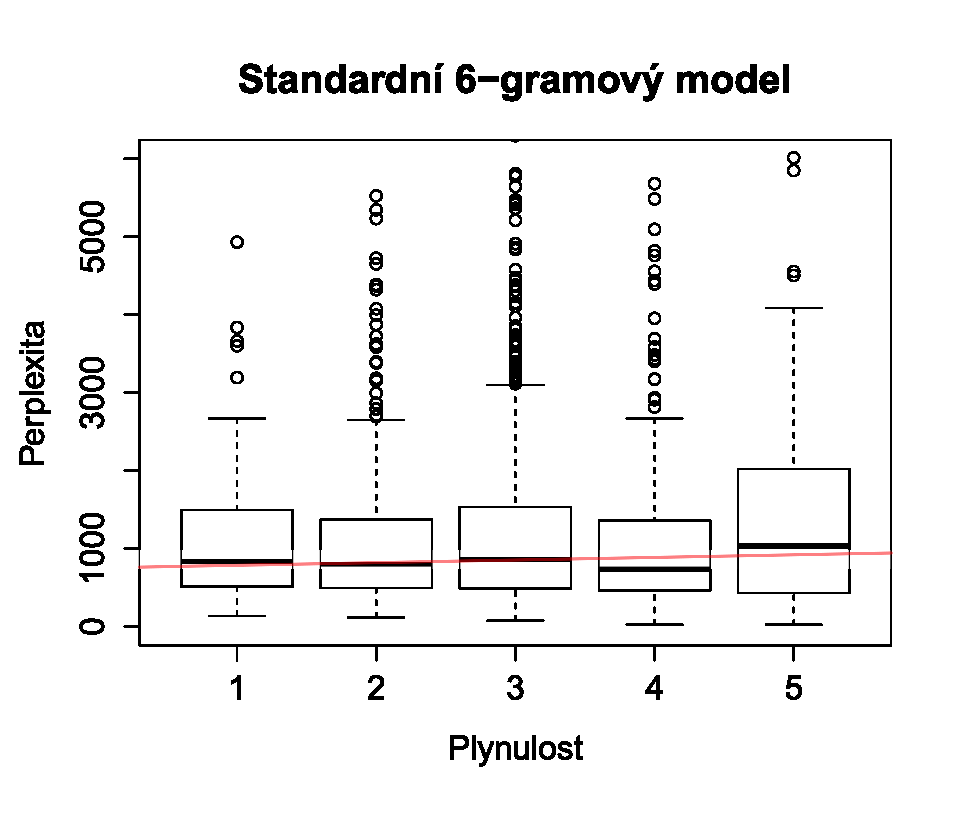
\includegraphics[width=60mm]{./grafy/morf/ngram/text.svg.eps}
  \caption{Standardní 6-gramový model se slovy}\label{gr:ngrslova}
\endminipage\quad
\minipage{0.45\textwidth}
  \centering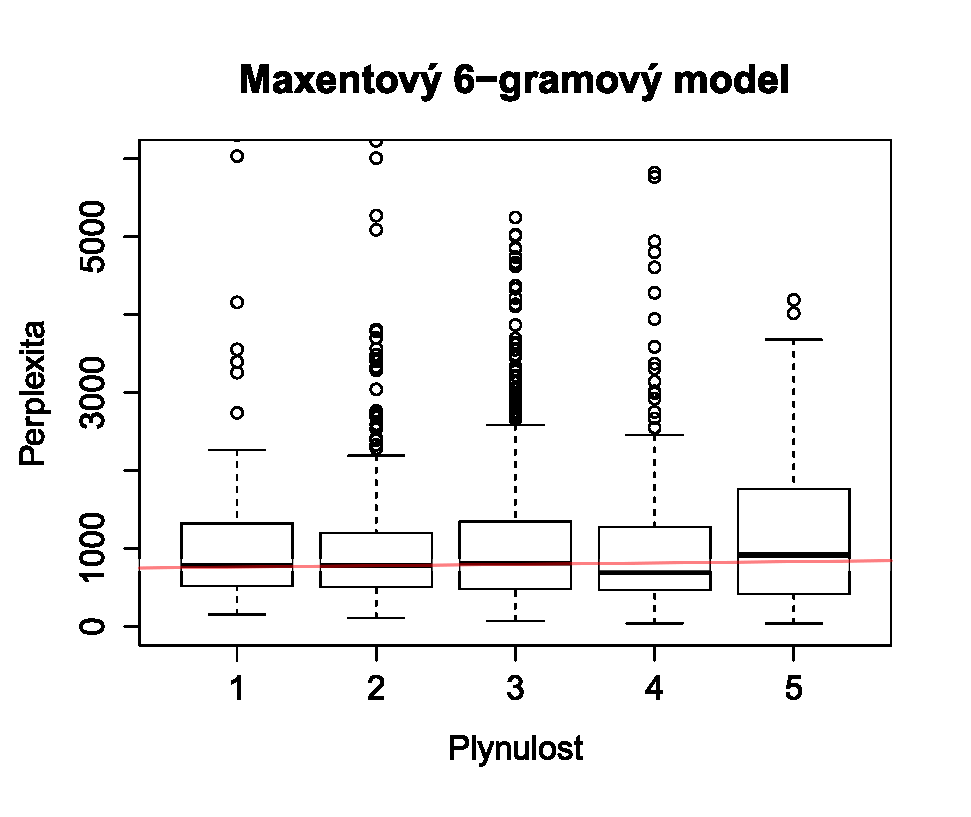
\includegraphics[width=60mm]{./grafy/morf/maxent/text.svg.eps}
  \caption{Maxentový 6-gramový model se slovy}\label{gr:maxslova}
\endminipage
\end{center}
\end{figure}


\pagebreak


Z obou grafů (obrázky \ref{gr:ngrslova}, \ref{gr:maxslova}) je patrné, že plynulost nekoreluje s perplexitou tak, jak bychom chtěli. Perplexita by měla se zvyšující se plynulostí klesat - čím nižší perplexita, tím lepší a tedy i plynulejší překlad. Na obou grafech však boxploty neklesají, nýbrž kolísají. Dokonce hypotézy hodnocené plynulostí 5 mají rozsah nejčastějších perplexit nejvyšší. To ale může být částečně způsobeno malým počtem hypotéz ohodnocených plynulostí 5.

\begin{figure}[!htbp]
\begin{center}
	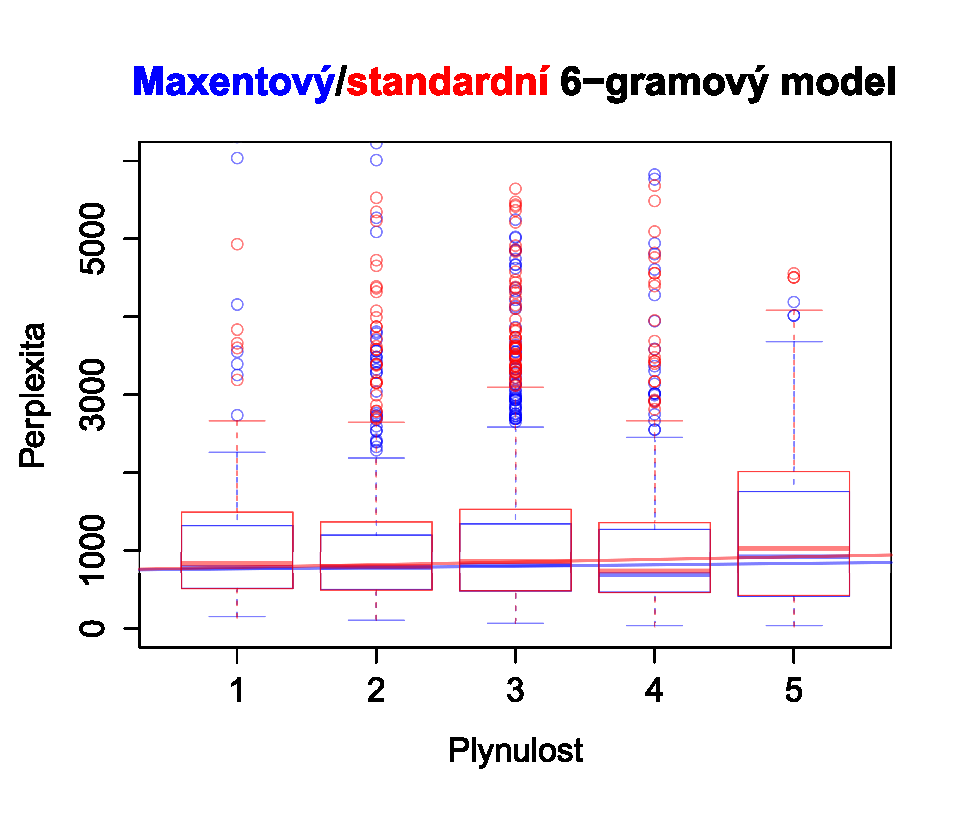
\includegraphics[width=90mm]{./grafy/morf/porovnani/text.svg.eps}
\end{center}
\caption{Porovnání modelů se slovy}\label{gr:porslova}
\end{figure}

Srovnání ukazuje, že maxentový model dopadl o něco lépe, neboť jednotlivé boxploty mají nižší horní hranici nejčastějších perplexit než v případě standardních modelů. Rozdíly ve spodních hranicích jsou zanedbatelné. I proložená přímka stoupá v případě standardního n-gramového modelu více než v případě maxentového (obrázek \ref{gr:porslova}).

Čas nutný k natrénování se však výrazně liší - natrénování standardního n-gramového trvalo zhruba 3 minuty oproti téměř 12 hodinám u modelu maxentového.

\section{Rozšířený slovní druh + morfologické značky}
Jako první zkusíme natrénovat model, kde slova nahradíme rozšířeným slovním druhem a všemi morfologickými značkami z výstupu ParZu. Pro oddělení použijeme dvojtečku.

Příklad věty:
\begin{center}
\texttt{%
\arrayrulecolor{seda}
\begin{tabular}{llll}
\color{red} Die & \color{red} unabhängige & \color{red} Justiz\\
\color{blue} ART:Def\textbar Fem\textbar Akk\textbar Sg & \color{blue} ADJA:Pos\textbar Fem\textbar Akk\textbar Sg\textbar \_\textbar & \color{blue} NN:Fem\textbar Akk\textbar Sg \\
\hline
\color{black}
\color{red} und & \color{red} die & \color{red} freien \\
\color{blue} KON:\_ & \color{blue} ART:Def\textbar Neut\textbar Akk\textbar Pl & \color{blue} ADJA:Pos\textbar Neut\textbar Akk\textbar Pl\textbar \_\textbar \\
\hline
\color{red} Medien & \color{red} zu & \color{red} unterdrücken & \color{red} . \\
\color{blue} NN:Neut\textbar Akk\textbar Pl & \color{blue} PTKZU:\_ & \color{blue} VVINF:\_ & \color{blue} \$.:\_ \\
\hline
\end{tabular}
}
\end{center}

\begin{figure}[!htb]
\begin{center}
\minipage{0.45\textwidth}
  \centering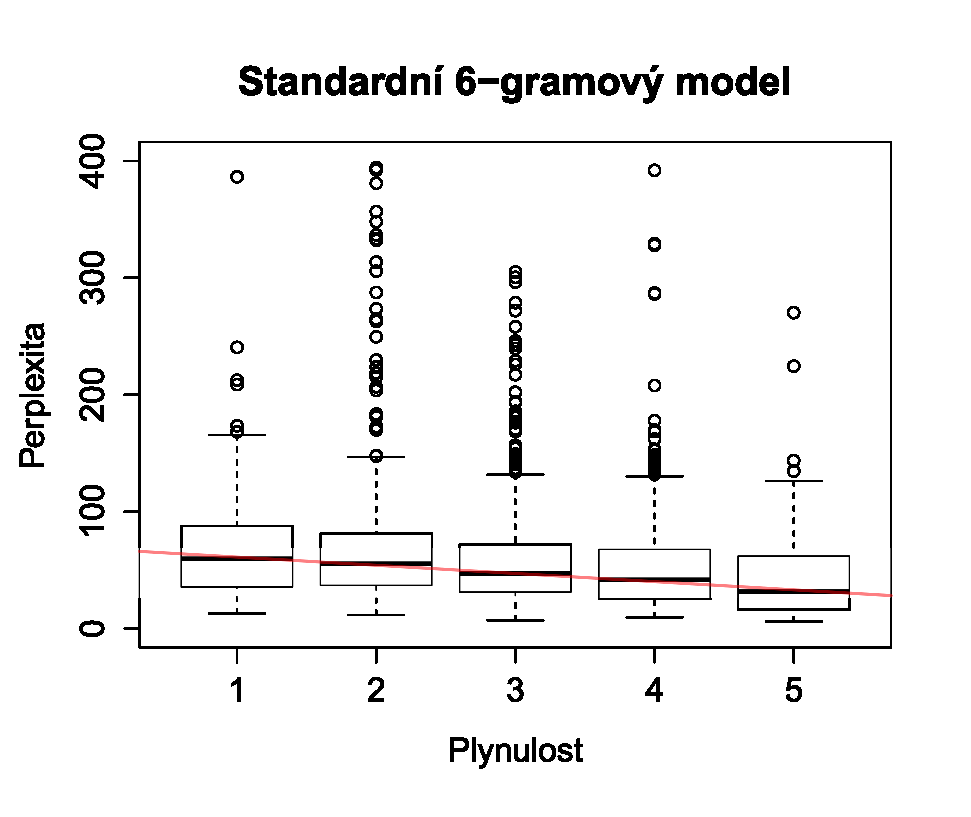
\includegraphics[width=60mm]{./grafy/morf/ngram/all.svg.eps}	
  \caption[Standardní 6-gramový model - rozšířený slovní druh + morf. zn.]{Standardní 6-gramový model - rozšířený slovní druh + morfologické značky}\label{gr:ngrrsd+morf}
\endminipage\quad
\minipage{0.45\textwidth}
  \centering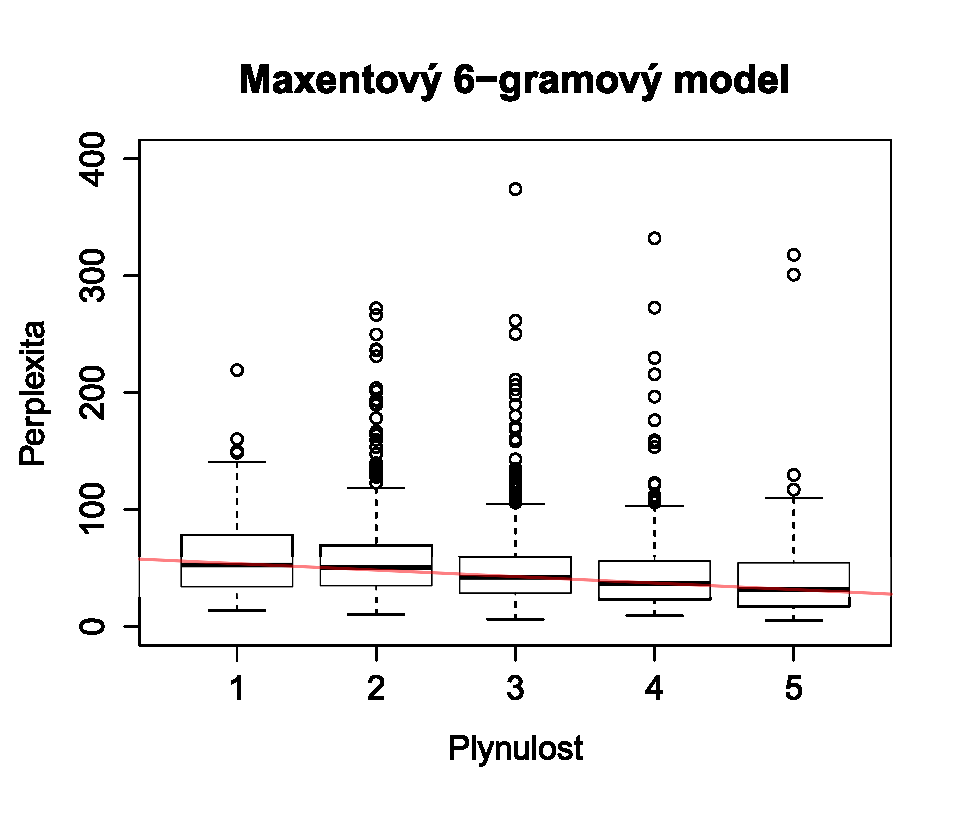
\includegraphics[width=60mm]{./grafy/morf/maxent/all.svg.eps}	
  \caption[Maxentový 6-gramový model - rozšířený slovní druh + morf. zn.]{Maxentový 6-gramový model - rozšířený slovní druh + morfologické značky}\label{gr:maxrsd+morf}
\endminipage
\end{center}
\end{figure}

Oba modely dopadly lépe než modely trénované na slovech. Boxploty vykazují lehce klesavou tendenci.

\pagebreak

\begin{figure}[!htbp]
\begin{center}
	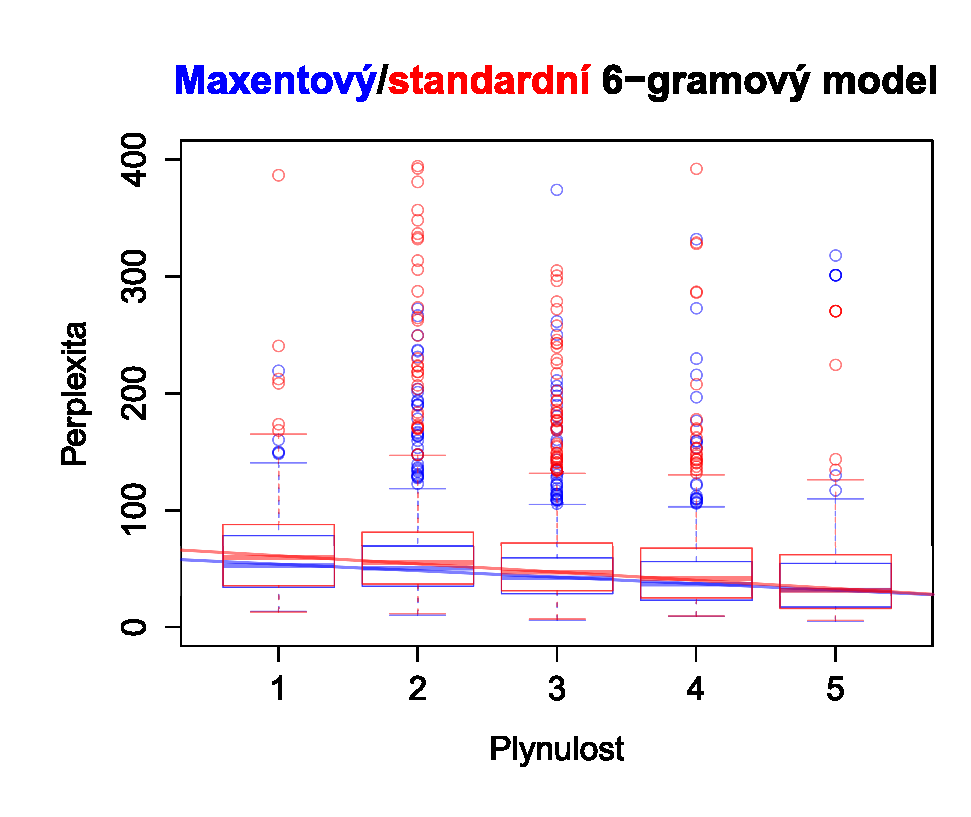
\includegraphics[width=90mm]{./grafy/morf/porovnani/all.svg.eps}	
\end{center}
\caption{Porovnání modelů - rozšířený slovní druh + morfologické značky}\label{gr:porrsd+morf}
\end{figure}


Maxentové modely opět, co se perplexity týče, dopadají lépe než standardní n-gramové. Avšak proložená přímka klesá u standardních modelů strměji. Z hlediska výpočetních nároků jsou na tom stadardní n-gramy oproti maxentovým znovu výrazně lépe - 72 sekund proti takřka 8 hodinám.

Tyto modely sice obsahují morfologickou analýzu, ale nerozumí jejímu obsahu. Nedokáží rozlišit, zda se sousední jména shodují v rodě, ale už ne v pádě apod. Natrénování maxentového modelu s rysy, které by vycházely z morfologické analýzy (rod, pád, číslo, ...), rozšíření SRILMu od Tanela Alumäe a Mikko Kurima bohužel neumožňuje a jiné dostupné toolkity, např. Maxent toolkit od LeZhanga, nejsou vhodné z hlediska výpočetních nároků na velká data. Zkusíme proto natrénovat další n-gramové modely, ve kterých nahradíme slova vždy jedním z potencionálních rysů. Takové modely by potom bylo možné kombinovat.

\section{Rozšířený slovní druh}
Zkusíme data ještě více zhustit a slova nahradit jen jejich rozšířeným slovním druhem.

Příklad věty:
\begin{center}
\texttt{%
\arrayrulecolor{seda}
\begin{tabular}{llll}
\color{red} Die & \color{red} unabhängige & \color{red} Justiz\\
\color{blue} ART & \color{blue} ADJA & \color{blue} NN \\
\hline
\color{black}
\color{red} und & \color{red} die & \color{red} freien \\
\color{blue} KON & \color{blue} ART & \color{blue} ADJA \\
\hline
\color{red} Medien & \color{red} zu & \color{red} unterdrücken & \color{red} . \\
\color{blue} NN & \color{blue} PTKZU & \color{blue} VVINF & \color{blue} \$. \\
\hline
\end{tabular}
}
\end{center}



\pagebreak



\begin{figure}[!htb]
\begin{center}
\minipage{0.45\textwidth}
  \centering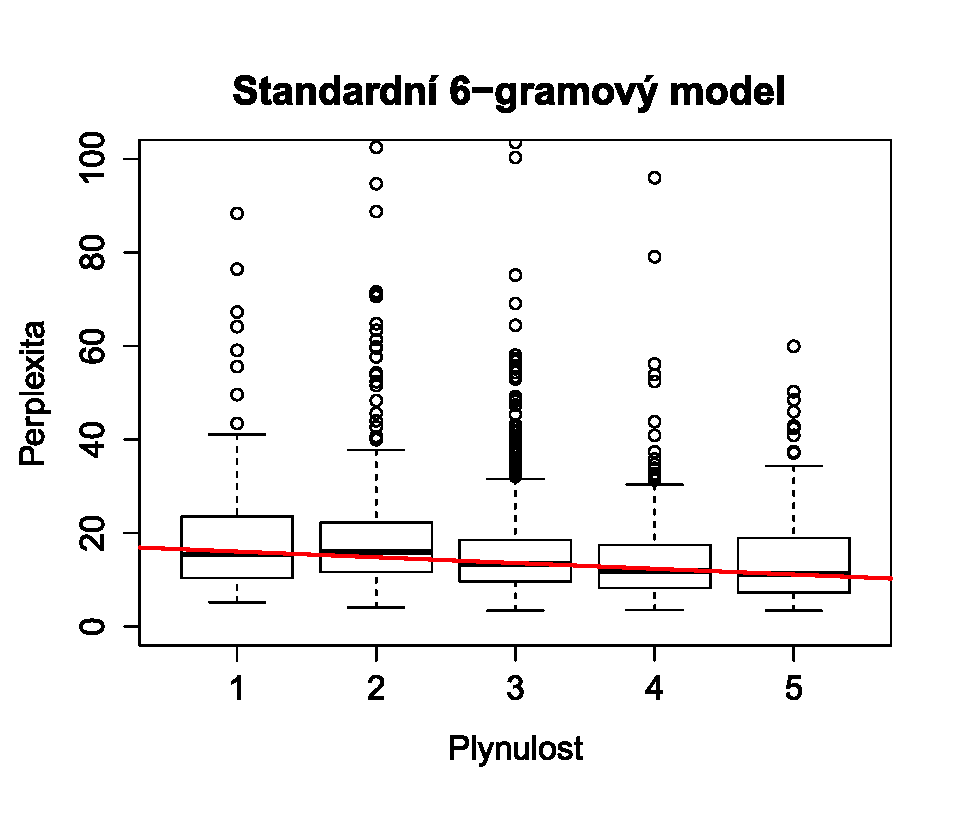
\includegraphics[width=60mm]{./grafy/morf/ngram/rsd.svg.eps}
  \caption{Standardní 6-gramový model - rozšířený slovní druh}\label{gr:ngrrsd}
\endminipage\quad
\minipage{0.45\textwidth}
  \centering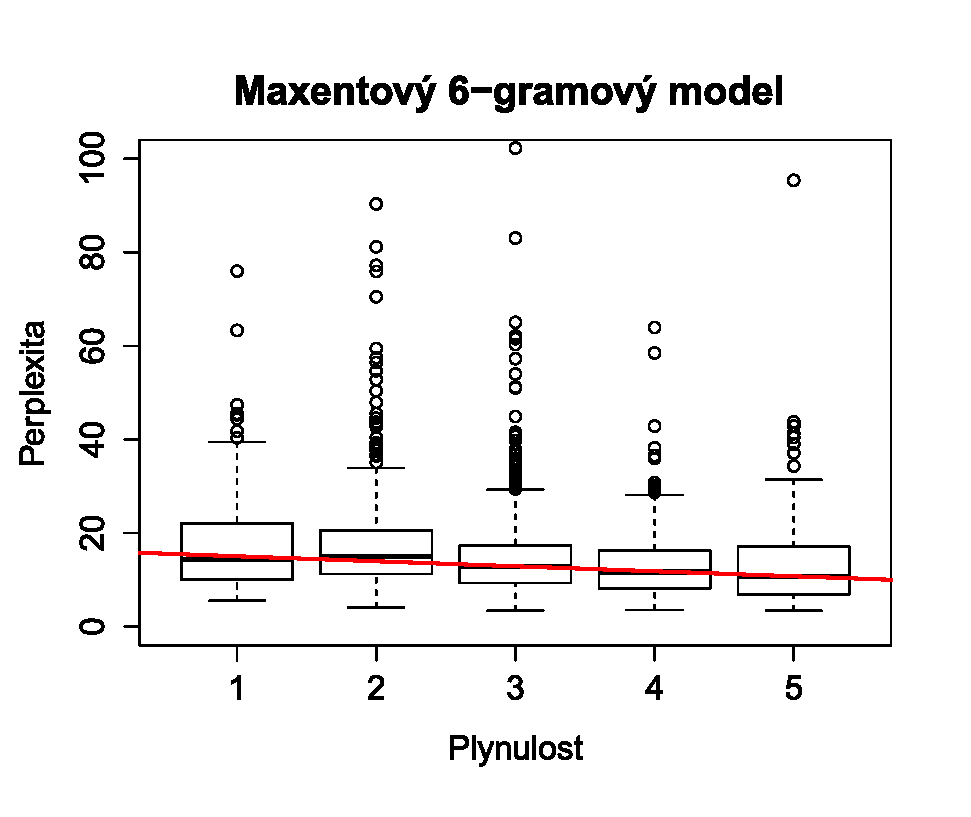
\includegraphics[width=60mm]{./grafy/morf/maxent/rsd.svg.eps}
  \caption{Maxentový 6-gramový model - rozšířený slovní druh}\label{gr:maxrsd}
\endminipage
\end{center}
\end{figure}


Modely dopadly o něco hůře než v případě, kdy byl rozšířený slovní druh ještě upřesněn další analýzou. Bez dalšího určení nemůžeme např. kontrolovat správné vyskloňování. Stále je to však lepší než při natrénování na slovech.

\begin{figure}[!htbp]
\begin{center}
	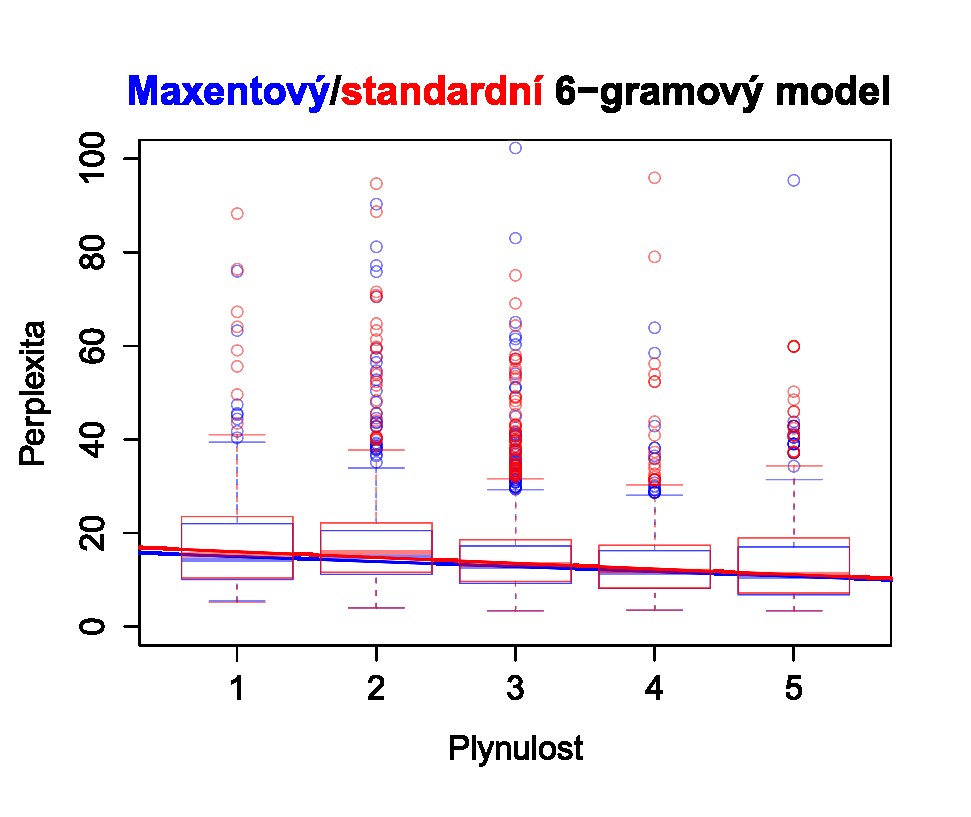
\includegraphics[width=90mm]{./grafy/morf/porovnani/rsd.svg.eps}	
\end{center}
\caption{Porovnání modelů - rozšířený slovní druh}\label{gr:porrsd}
\end{figure}

V porovnání je na tom maxentový model z hlediska perplexity opět mírně lépe. Stejně jako proložená přímka klesá u standardního n-gramového modelu strměji (obrázek \ref{gr:porrsd}).

Z hlediska výpočetních nároků to tentokrát není takový rozdíl. Standardní n-gramový model potřeboval pro natrénování 22 sekund, maxentový 14 minut.

Zde je vidět, nakolik ovlivňuje velikost slovníku dobu trénování maxentových modelů. Oproti modelům se všemi morfologickými značkami potřebovaly standardní n-gramy 3.27x méně času, maxentové 34.29x, což je obrovský rozdíl.

\section{Rod}
První z modelů s jedinou morfologickou značkou budou modely obsahující rod. Slova budou nahrazena znakem \texttt{w}, ke kterému se připojí patřičný rod, lze-li u slova určit. Tím dojde ke zhuštění dat a velikost slovníku se zmenší na pouhá 4 slova.

Příklad věty:
\begin{center}
\texttt{%
\arrayrulecolor{seda}
\begin{tabular}{lllllll}
\color{red} Die & \color{red} unabhängige & \color{red} Justiz & \color{red} und & \color{red} die & \color{red} freien & \color{red} Medien\\
\color{blue} wFem & \color{blue} wFem & \color{blue} wFem & \color{blue} w & \color{blue} wNeut & \color{blue} wNeut & \color{blue} wNeut\\
\hline
\color{red} zu & \color{red} unterdrücken &\color{red} .\\
\color{blue} w & \color{blue} w & \color{blue} w \\
\hline
\end{tabular}
}
\end{center}

\begin{figure}[!htb]
\begin{center}
\minipage{0.45\textwidth}
  \centering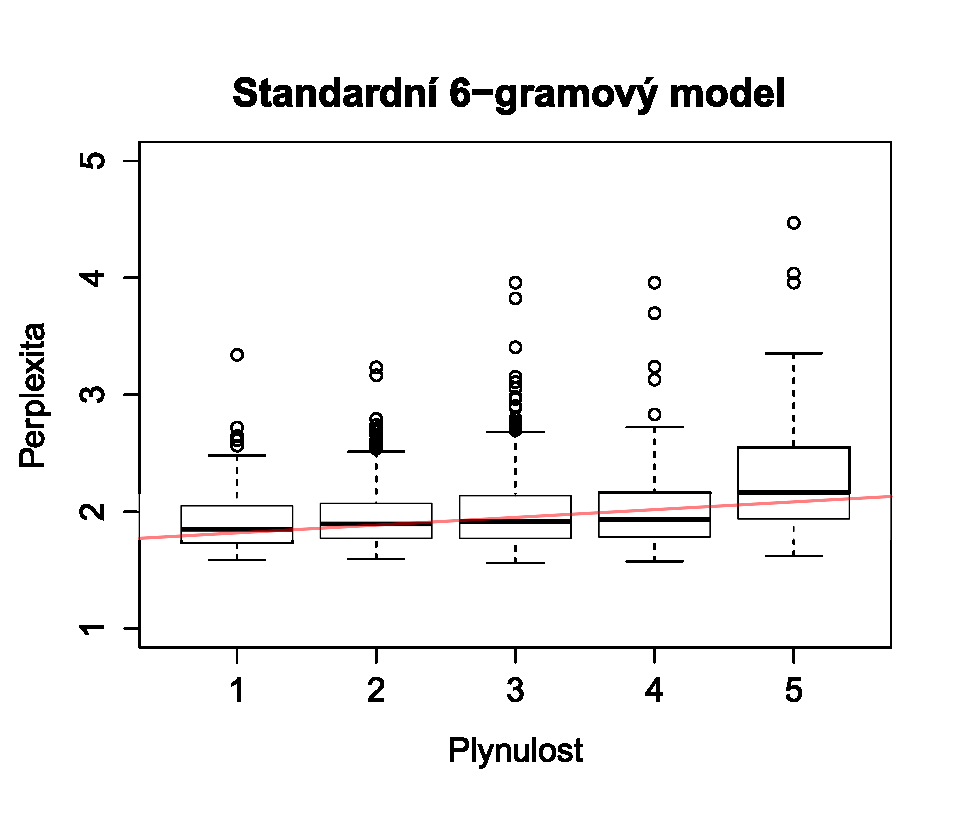
\includegraphics[width=60mm]{./grafy/morf/ngram/rod.svg.eps}
  \caption{Standardní 6-gramový model - rod}\label{gr:ngrrod}
\endminipage\quad
\minipage{0.45\textwidth}
  \centering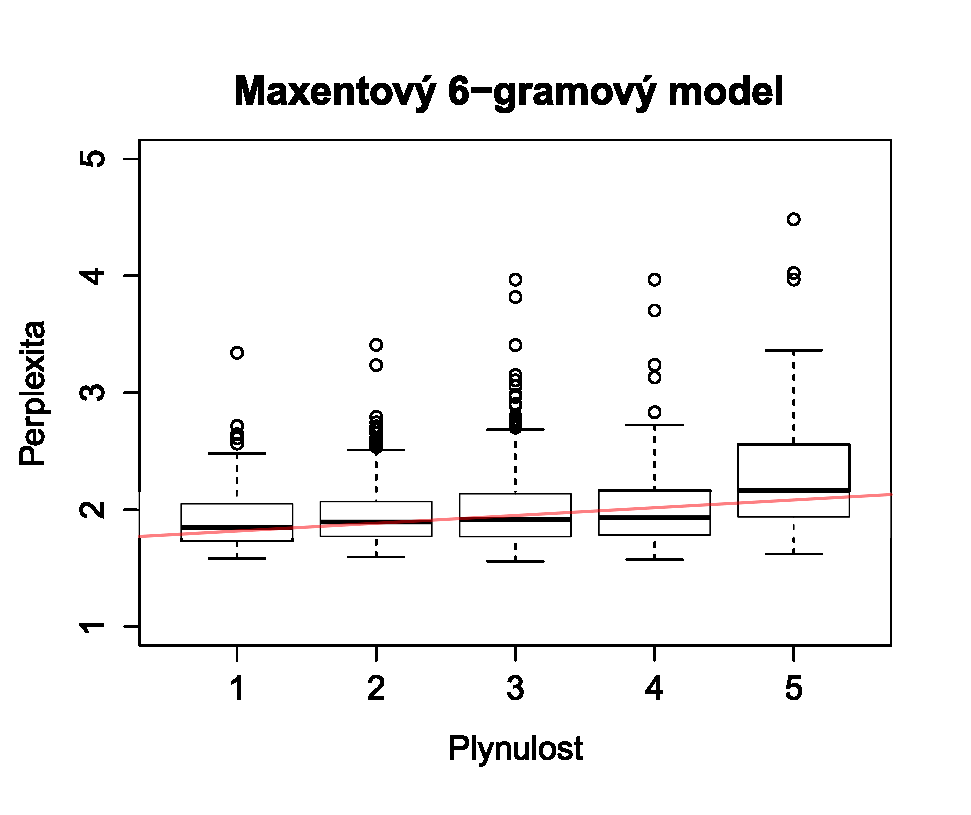
\includegraphics[width=60mm]{./grafy/morf/maxent/rod.svg.eps}
  \caption{Maxentový 6-gramový model - rod}\label{gr:maxrod}
\endminipage
\end{center}
\end{figure}

Modely ale dopadly přesně obráceně, než jsme chtěli. Boxploty neklesají, ale stoupají (obrázky \ref{gr:ngrrod}, \ref{gr:maxrod}). S trochou nadsázky by se dalo říct, že zde čím je perplexita vyšší, tím je lepší plynulost. Ovšem skutečnost je taková, že perplexita pro plynulosti 1-4 vyšla velmi podobně a nejsme pouze na základě ní schopni rozlišit, o kterou plynulost by se mělo jednat.


\pagebreak



\begin{figure}[!htbp]
\begin{center}
	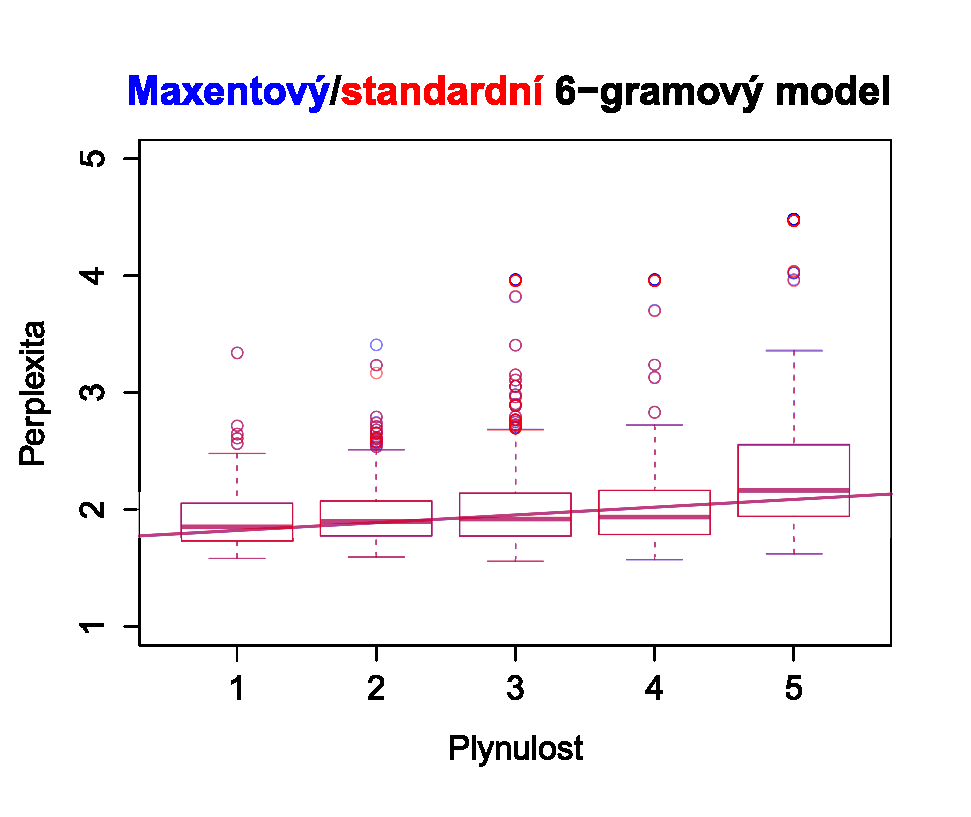
\includegraphics[width=90mm]{./grafy/morf/porovnani/rod.svg.eps}	
\end{center}
\caption{Porovnání modelů - rod}\label{gr:porrod}
\end{figure}

Rozdíl mezi standardními a maxentovými n-gramovými modely je prakticky neznatelný (obrázek \ref{gr:porrod}). Stejně je tomu tentokrát i u výpočetních nároků. Standardní n-gramy potřebovaly k natrénování 3 sekundy, maxentové n-gramy pak sekundy 4.

\subsection{Rod stejný s předchozím}
Ačkoliv modely pouze s rodem nebyly úspěšné, zkusíme ještě slova nenahrazovat jenom rodem daného slova, ale pokusíme se sledovat, zda se rody za sebou shodují. Slova tedy nahradíme opět písmenem \texttt{w}, k němuž přidáme slovo \texttt{rod}, lze-li u slova určit, a slovo \texttt{stejne}, pokud lze jednak rod u slova určit a jednak, pokud se rod shoduje s předchozím slovem.


Příklad věty:
\begin{center}
\texttt{%
\arrayrulecolor{seda}
\begin{tabular}{lllllll}
\color{red} Die & \color{red} unabhängige & \color{red} Justiz & \color{red} und & \color{red} die & \color{red} freien & \color{red} Medien\\
\color{blue} wrod & \color{blue} wstejny & \color{blue} wstejny & \color{blue} w & \color{blue} wrod & \color{blue} wstejny & \color{blue} wstejny\\
\hline
\color{red} zu & \color{red} unterdrücken &\color{red} .\\
\color{blue} w & \color{blue} w & \color{blue} w \\
\hline
\end{tabular}
}
\end{center}


\pagebreak


\begin{figure}[!htb]
\begin{center}
\minipage{0.45\textwidth}
  \centering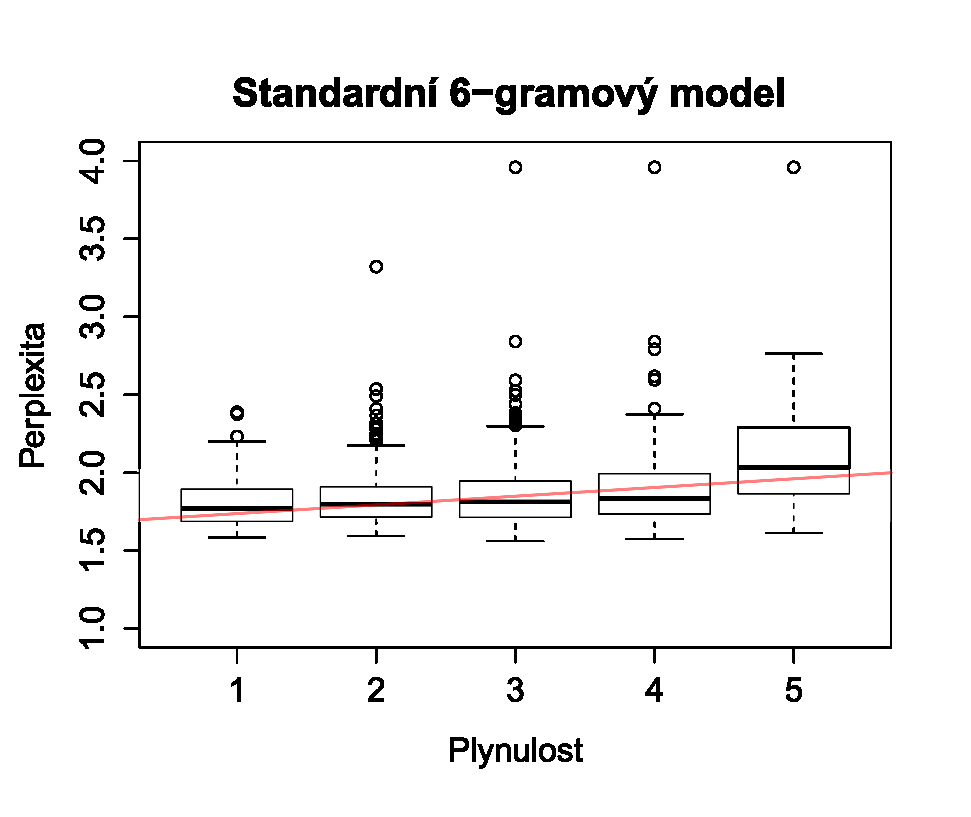
\includegraphics[width=60mm]{./grafy/morf/ngram/rodstejny.eps}
  \caption{Standardní 6-gramový model - rod stejný s předchozím}\label{gr:ngrrodstejny}
\endminipage\quad
\minipage{0.45\textwidth}
  \centering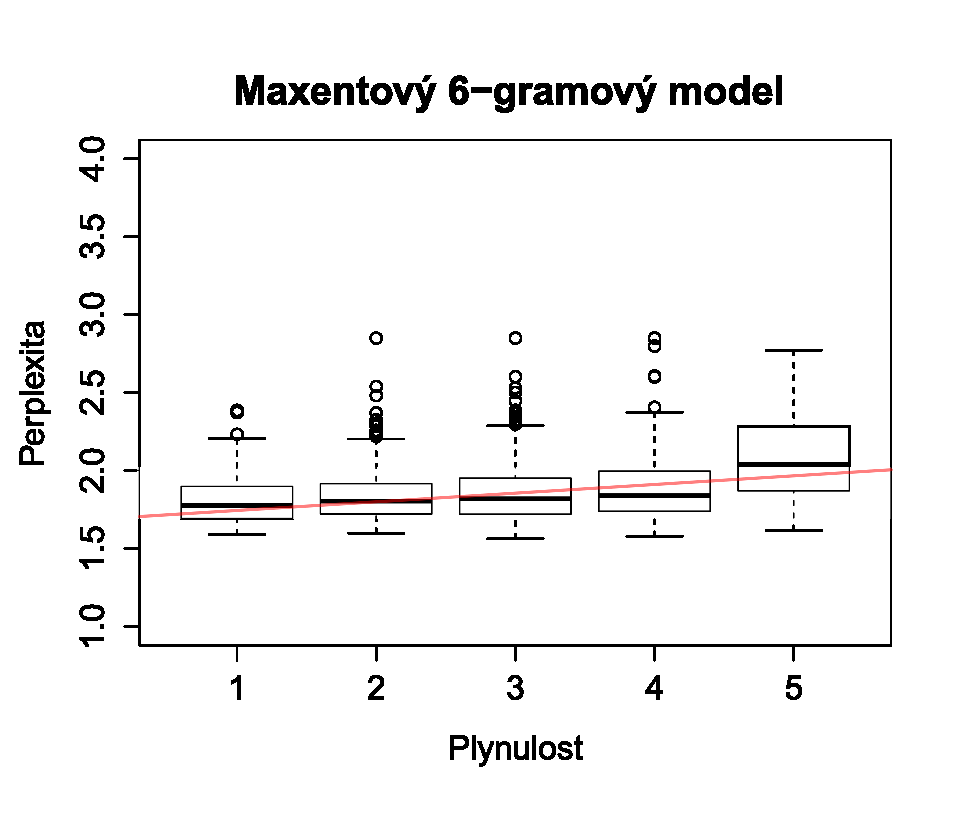
\includegraphics[width=60mm]{./grafy/morf/maxent/rodstejny.eps}
  \caption{Maxentový 6-gramový model - rod stejný s předchozím}\label{gr:maxrodstejny}
\endminipage
\end{center}
\end{figure}

Výsledky jsou ale stejně špatné jako v případě samotného rodu. Grafy se sobě velmi podobají (obrázek \ref{gr:ngrrodstejny}, \ref{gr:maxrodstejny}).

\begin{figure}[!htbp]
\begin{center}
	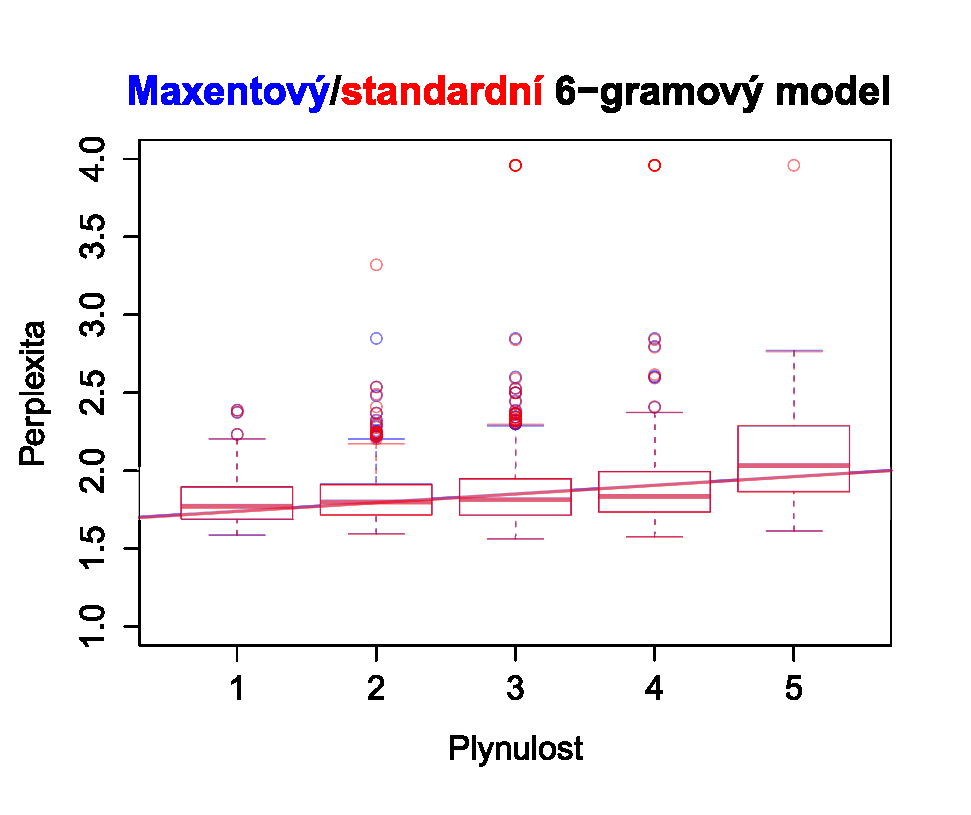
\includegraphics[width=90mm]{./grafy/morf/porovnani/rodstejny.eps}	
\end{center}
\caption{Porovnání modelů - rod stejný s předchozím}\label{gr:porrodstejny}
\end{figure}

Rozdíly mezi standardním n-gramovým a maxentovým n-gramovým modelem je taktéž nepatrný (obrázek \ref{gr:porrodstejny}). Doba nutná k natrénování obou typů byla v tomto případě shodně 3 sekundy.

\subsection{S rozšířeným slovním druhem}
Jelikož samotný rod byla pro model nedostatečná informace, zkusíme namísto písmene \texttt{w} slova nahrazovat rozšířeným slovním druhem a k němu přidávat za dvojtečku rod.

Příklad věty:
\begin{center}
\texttt{%
\arrayrulecolor{seda}
\begin{tabular}{lllllll}
\color{red} Die & \color{red} unabhängige & \color{red} Justiz & \color{red} und & \color{red} die & \color{red} freien & \color{red} Medien\\
\color{blue} ART:Fem & \color{blue} ADJA:Fem & \color{blue} NN:Fem & \color{blue} KON & \color{blue} ART:Neut & \color{blue} ADJA:Neut & \color{blue} NN:Neut\\
\hline
\color{red} zu & \color{red} unterdrücken &\color{red} .\\
\color{blue} PTKZU & \color{blue} VVINF & \color{blue} \$. \\
\hline
\end{tabular}
}
\end{center}

\begin{figure}[!htb]
\begin{center}
\minipage{0.45\textwidth}
  \centering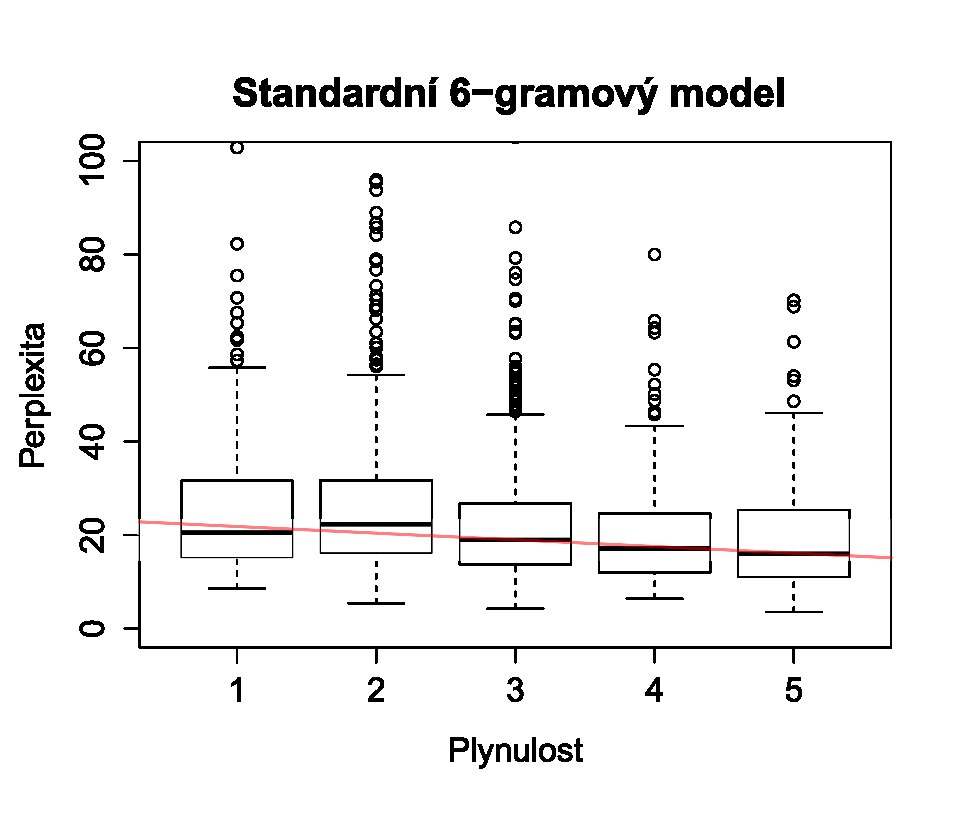
\includegraphics[width=60mm]{./grafy/morf/ngram/rsd+rod.svg.eps}
  \caption{Standardní 6-gramový model - číslo}\label{gr:ngrcislo}
\endminipage\quad
\minipage{0.45\textwidth}
  \centering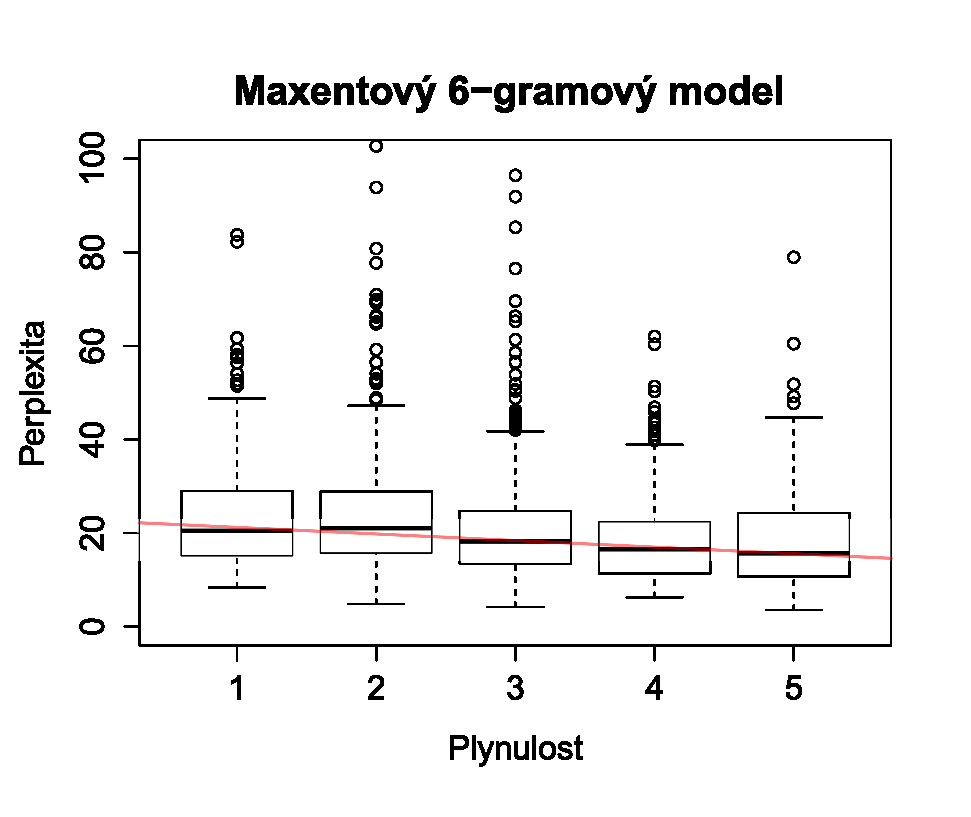
\includegraphics[width=60mm]{./grafy/morf/maxent/rsd+rod.svg.eps}
  \caption{Maxentový 6-gramový model - číslo}\label{gr:maxcislo}
\endminipage
\end{center}
\end{figure}


S rozšířeným slovním druhem už modely dopadly lépe, přesto perplexita s rostoucí plynulostí neklesá nijak výrazně, což dokazuje proložená přímka.

\begin{figure}[!htbp]
\begin{center}
	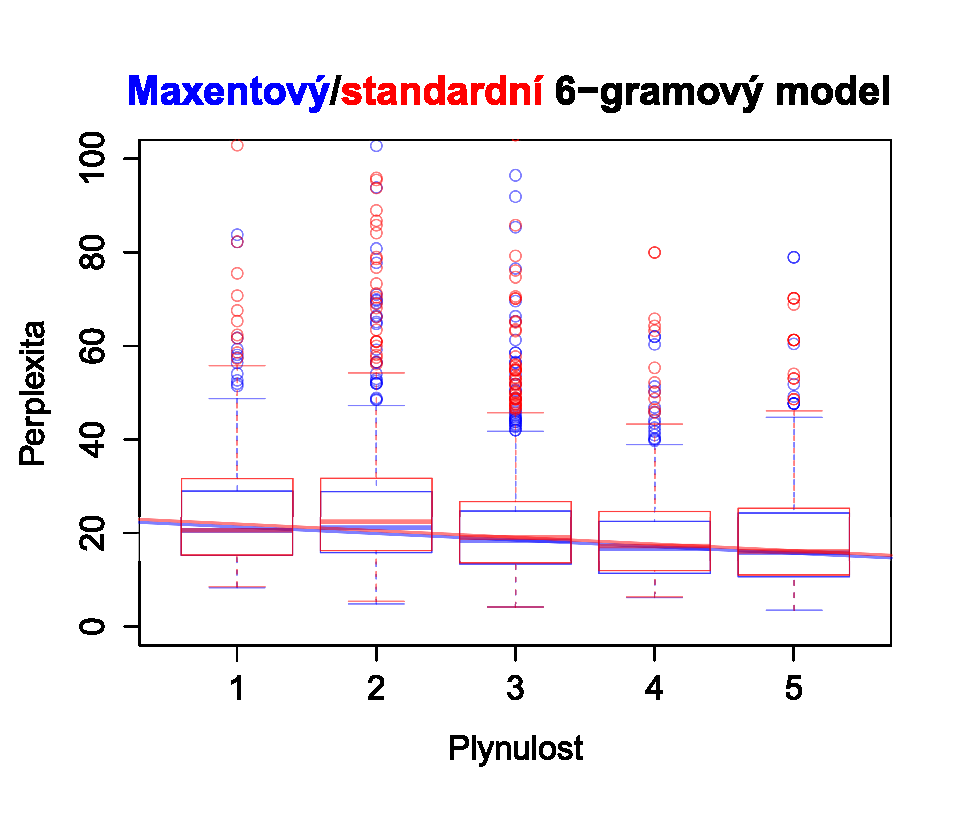
\includegraphics[width=90mm]{./grafy/morf/porovnani/rsd+rod.svg.eps}	
\end{center}
\caption{Porovnání modelů - rozšířený slovní druh + rod}\label{gr:porrsd+rod}
\end{figure}

Ve srovnání jsou oba typy modelů na tom podobně, maxentové dostávaly jen o něco málo nižší perplexitu (obrázek \ref{gr:porrsd+rod}). Z hlediska výpočetní náročnosti je ale rozdíl velký - 36 sekund standardní n-gramový model naproti 27 minutám u modelu maxentového.

\section{Číslo}
Stejné modely zkusíme natrénovat i v případě čísla. Jako první znovu zkusíme, zda bude modelu postačovat informace pouze o čísle daného slova tj. \texttt{wSg}, \texttt{wPl} nebo \texttt{w}.

Příklad věty:
\begin{center}
\texttt{%
\arrayrulecolor{seda}
\begin{tabular}{lllllll}
\color{red} Die & \color{red} unabhängige & \color{red} Justiz & \color{red} und & \color{red} die & \color{red} freien & \color{red} Medien\\
\color{blue} wSg & \color{blue} wSg & \color{blue} wSg & \color{blue} w & \color{blue} wPl & \color{blue} wPl & \color{blue} wPl\\
\hline
\color{red} zu & \color{red} unterdrücken &\color{red} .\\
\color{blue} w & \color{blue} w & \color{blue} w \\
\hline
\end{tabular}
}
\end{center}

\begin{figure}[!htb]
\begin{center}
\minipage{0.45\textwidth}
  \centering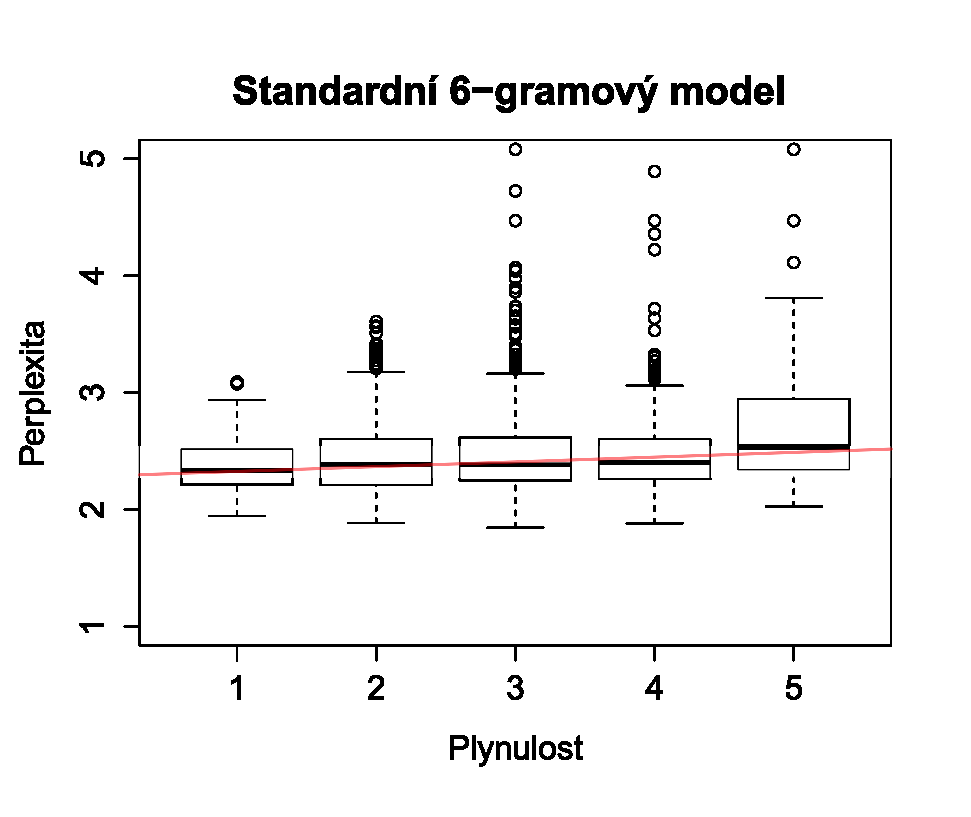
\includegraphics[width=60mm]{./grafy/morf/ngram/cislo.svg.eps}
  \caption{Standardní 6-gramový model - číslo}\label{gr:ngrcislo}
\endminipage\quad
\minipage{0.45\textwidth}
  \centering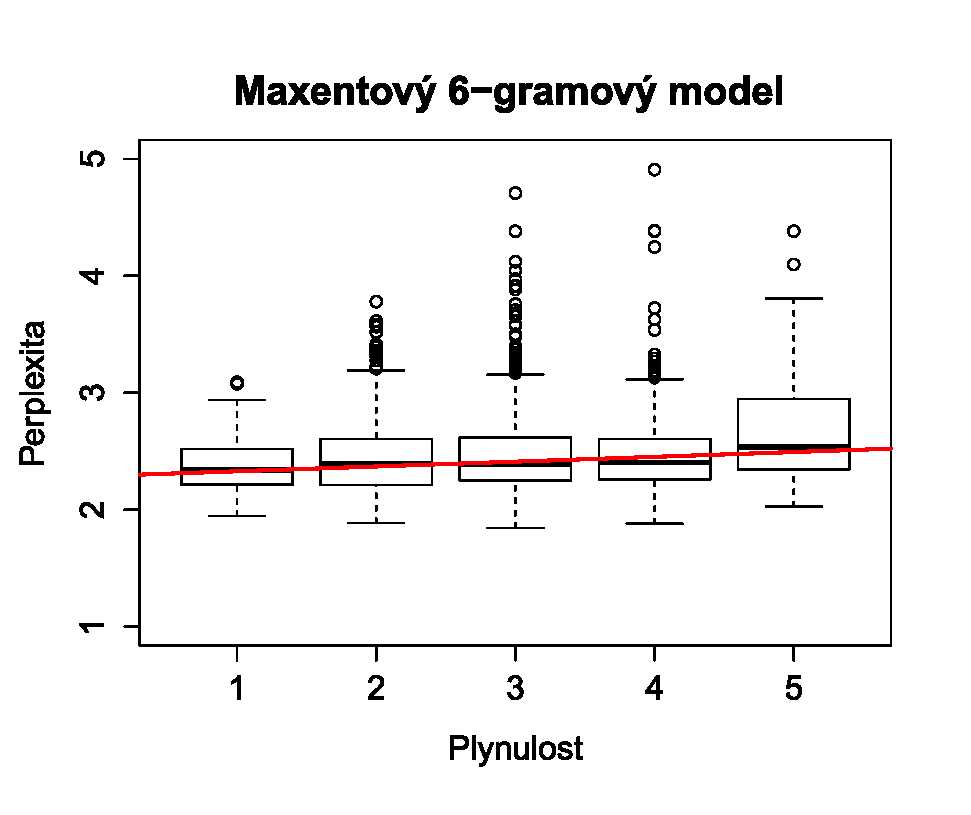
\includegraphics[width=60mm]{./grafy/morf/maxent/cislo.svg.eps}	
  \caption{Maxentový 6-gramový model - číslo}\label{gr:maxcislo}
\endminipage
\end{center}
\end{figure}


Výsledky ale dopadly obdobně špatně jako v případě rodu. Pomocí perplexity nejsme schopni rozlišit, o jakou plynulost by se mělo jednat.

\begin{figure}[!htbp]
\begin{center}
	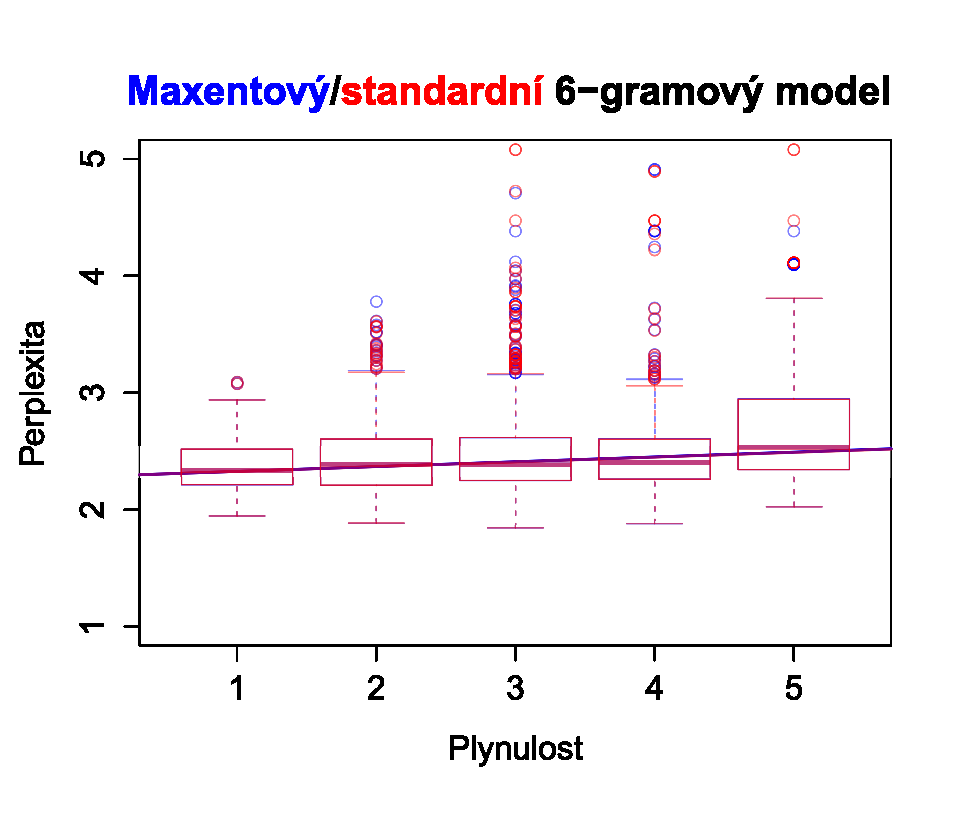
\includegraphics[width=90mm]{./grafy/morf/porovnani/cislo.svg.eps}
\end{center}
\caption{Porovnání modelů - číslo}\label{gr:porcislo}
\end{figure}

Oba typy modelů dopadly takřka stejně (obrázek \ref{gr:porcislo}). Stejná byla i doba nutná k natrénování - shodně po třech sekundách.

\subsection{Přidání osoby}
Číslo se bude často pojit s nějakou osobou. Zkusíme proto tuto informaci k číslu přidat. Slovo nahradíme písmenem \texttt{w}, poté bude následovat osoba a číslo, jdou-li u daného slova určit.

Příklad věty:
\begin{center}
\texttt{%
\arrayrulecolor{seda}
\begin{tabular}{llllll}
\color{red} Zur & \color{red} Belohnung & \color{red} erhielt & \color{red} Pakistan & \color{red} von & \color{red} Amerika\\
\color{blue} w & \color{blue} wSg & \color{blue} w3Sg & \color{blue} wSg & \color{blue} w & \color{blue} wSg\\
\hline
\color{red} finanzielle & \color{red} Unterstützung & \color{red} und &\color{red} Waffen &\color{red} .\\
\color{blue} wSg & \color{blue} wSg & \color{blue} w & \color{blue} wPl & \color{blue} w \\
\hline
\end{tabular}
}
\end{center}

\begin{figure}[!htb]
\begin{center}
\minipage{0.45\textwidth}
  \centering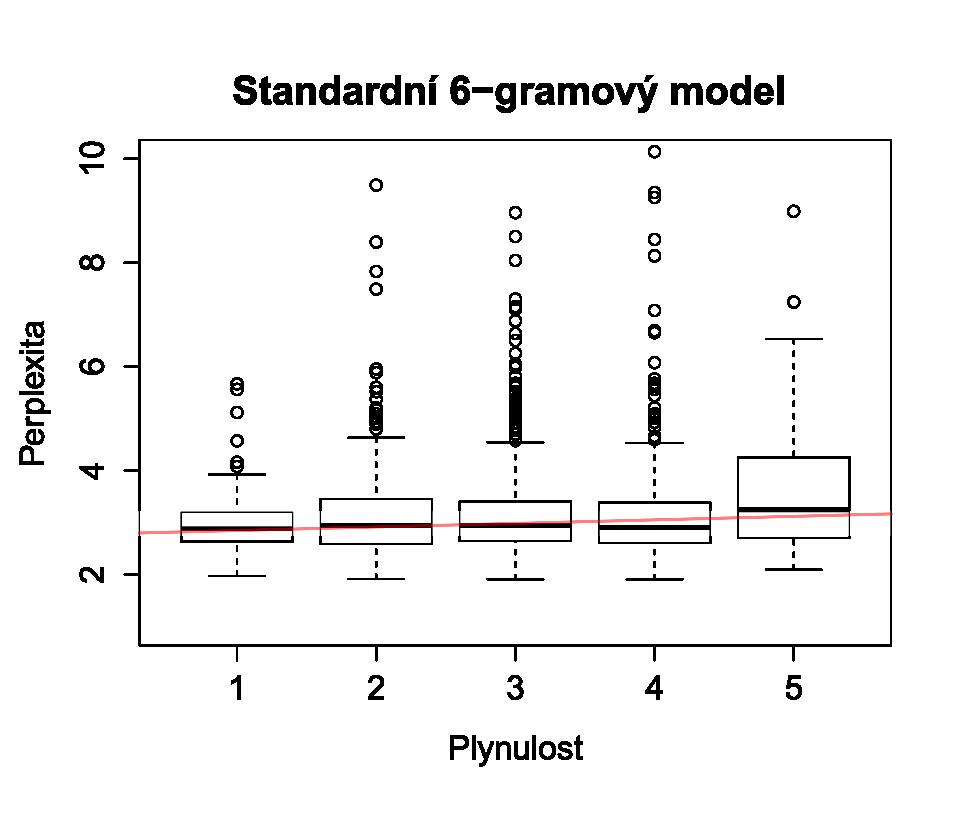
\includegraphics[width=60mm]{./grafy/morf/ngram/osoba+cislo.svg.eps}
  \caption{Standardní 6-gramový model - osoba + číslo}\label{gr:ngros+cislo}
\endminipage\quad
\minipage{0.45\textwidth}
  \centering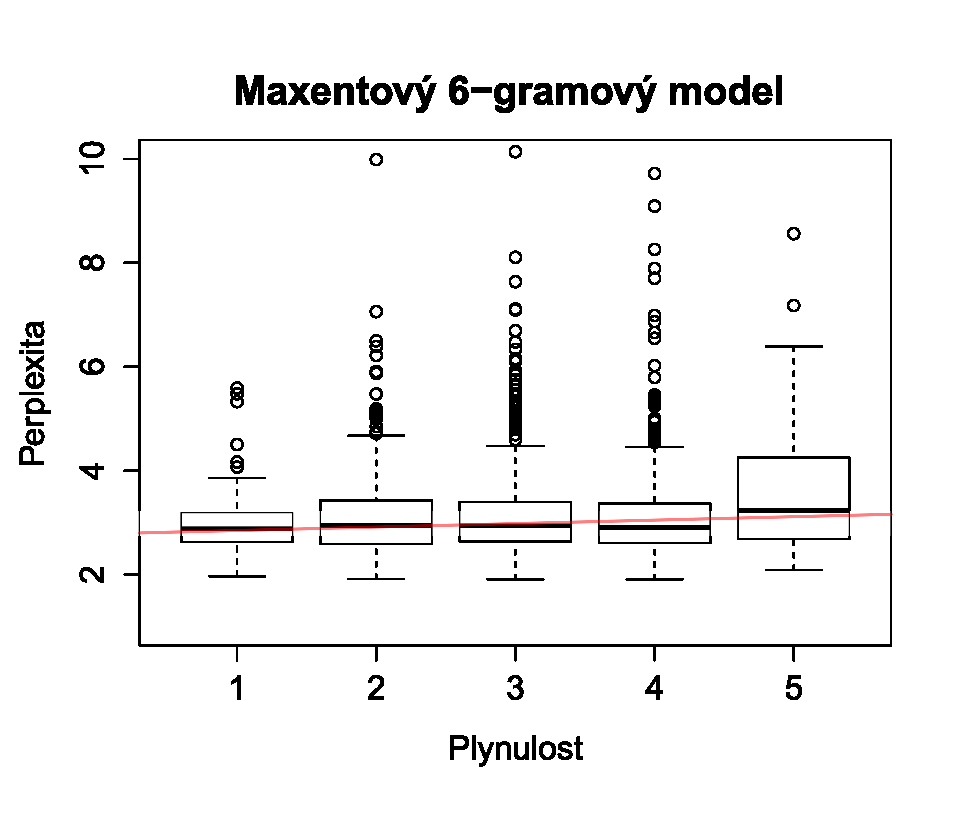
\includegraphics[width=60mm]{./grafy/morf/maxent/osoba+cislo.svg.eps}	
  \caption{Maxentový 6-gramový model - osoba + číslo}\label{gr:maxos+cislo}
\endminipage
\end{center}
\end{figure}

Modely ale nedopadly o nic lépe. Proložené přímky opět mírně stoupají, namísto aby klesaly (obrázky \ref{gr:ngros+cislo}, \ref{gr:maxos+cislo}).

\begin{figure}[!htbp]
\begin{center}
	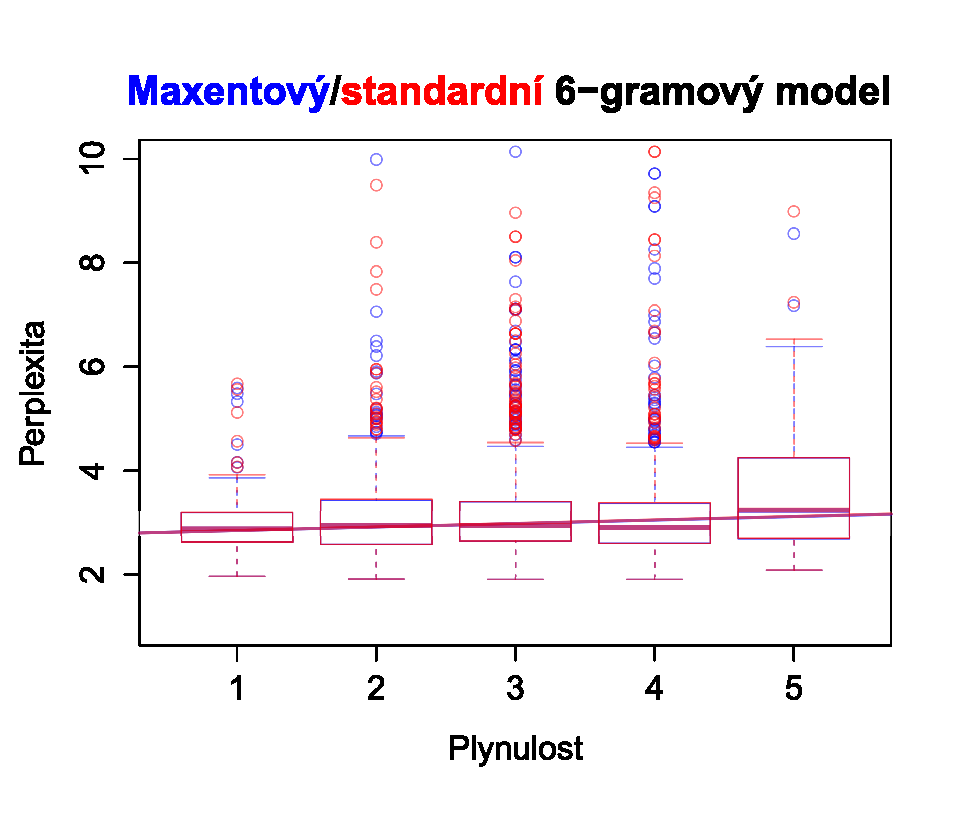
\includegraphics[width=90mm]{./grafy/morf/porovnani/osoba+cislo.svg.eps}	
\end{center}
\caption{Porovnání modelů - osoba + číslo}\label{gr:porosoba+cislo}
\end{figure}

Ve srovnání obou typů modelů opět nejsou patrné výrazné rozdíly (obrázek \ref{gr:porosoba+cislo}). Z hlediska výpočetních nároků se ale tentokrát trochu liší. Standardní n-gramové potřebovaly k natrénování 4 sekundy, maxentové 11 sekund.

\subsection{S rozšířeným slovním druhem}
Vzhledem k tomu, že přidání osoby žádné patrné zlepšení nepřineslo, zkusíme znovu přidat rozšířený slovní druh. Slova tedy budeme nahrazovat jejich druhem a číslem, lze-li určit.

Příklad věty:
\begin{center}
\texttt{%
\arrayrulecolor{seda}
\begin{tabular}{llllll}
\color{red} Zur & \color{red} Belohnung & \color{red} erhielt & \color{red} Pakistan & \color{red} von & \color{red} Amerika\\
\color{blue} APPRART & \color{blue} NN:Sg & \color{blue} VVFIN:Sg & \color{blue} NE:Sg & \color{blue} APPR & \color{blue} NE:Sg\\
\hline
\color{red} finanzielle & \color{red} Unterstützung & \color{red} und &\color{red} Waffen &\color{red} .\\
\color{blue} ADJA:Sg & \color{blue} NN:Sg & \color{blue} KON & \color{blue} NN:Pl & \color{blue} \$. \\
\hline
\end{tabular}
}
\end{center}


\pagebreak


\begin{figure}[!htb]
\begin{center}
\minipage{0.45\textwidth}
  \centering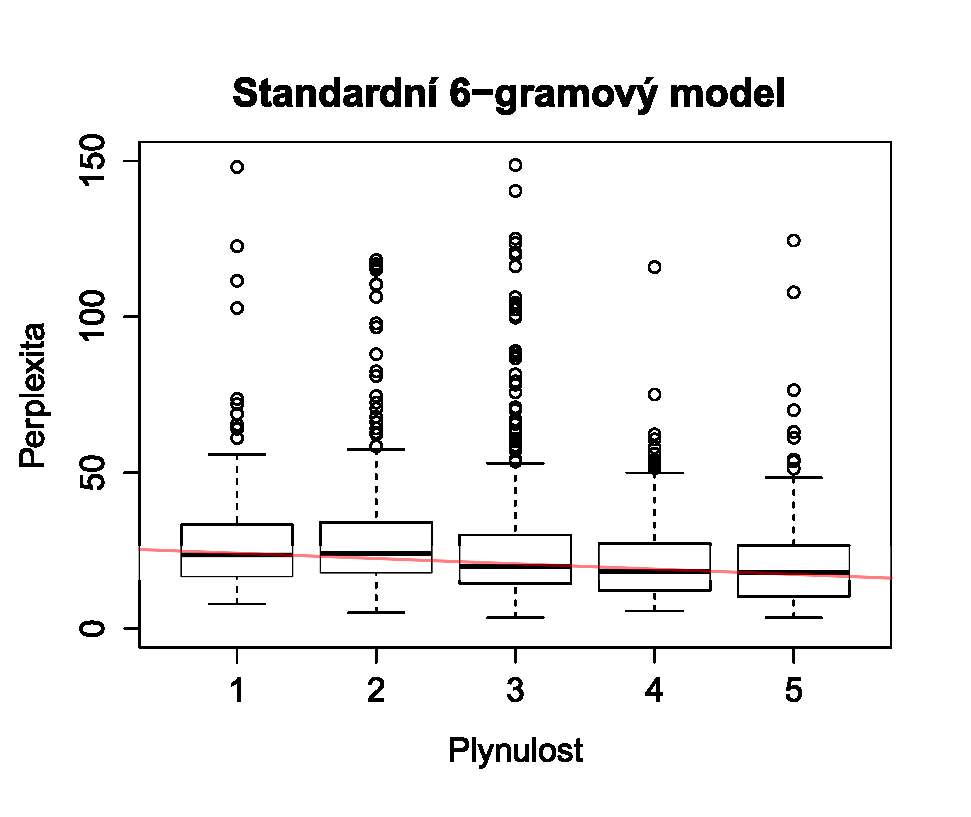
\includegraphics[width=60mm]{./grafy/morf/ngram/rsd+cislo.svg.eps}
  \caption{Standardní 6-gramový model - rozšířený slovní druh + číslo}\label{gr:ngrrsd+cislo}
\endminipage\quad
\minipage{0.45\textwidth}
  \centering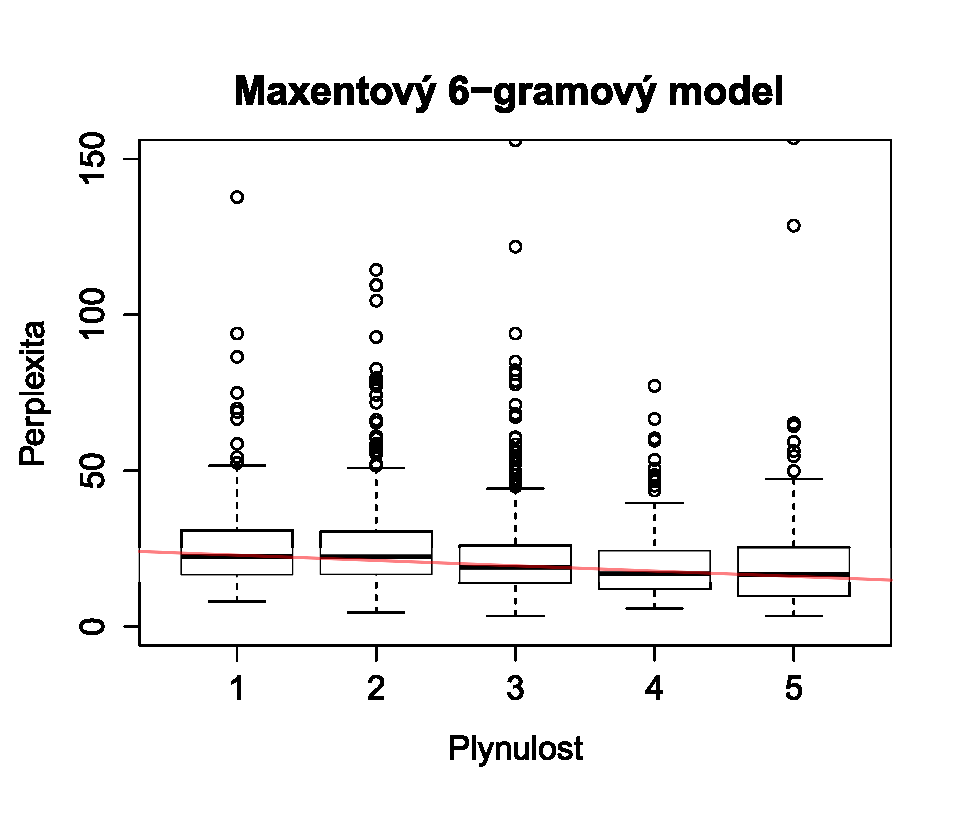
\includegraphics[width=60mm]{./grafy/morf/maxent/rsd+cislo.svg.eps}
  \caption{Maxentový 6-gramový model - rozšířený slovní druh + číslo}\label{gr:maxrsd+cislo}
\endminipage
\end{center}
\end{figure}




Modely s rozšířeným slovním druhem dopadly znovu lépe. Ovšem výsledky stále nejsou nijak dobré.

\begin{figure}[!htbp]
\begin{center}
	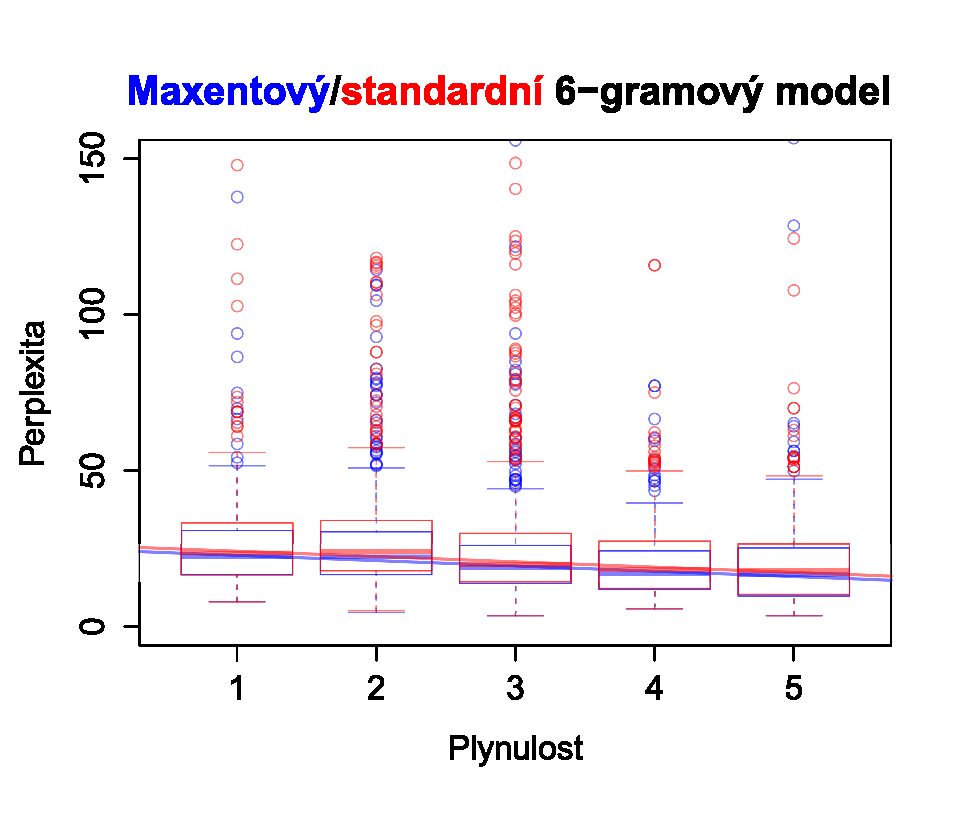
\includegraphics[width=90mm]{./grafy/morf/porovnani/rsd+cislo.svg.eps}	
\end{center}
\caption{Porovnání modelů - rozšířený slovní druh + číslo}\label{gr:porrsd+cislo}
\end{figure}

V porovnání dostávaly maxentové modely o něco nižší perplexitu. Čas potřebný k natrénování byl u standardních n-gramových modelů 33 s, u maxentových 24 minut.

\section{Pád}
Jako poslední zkusíme ještě natrénovat modely, kde slova nahradíme znovu písmenem \texttt{w} a přidáme k němu pád, lze-li u daného slova určit.

Příklad věty:
\begin{center}
\texttt{%
\arrayrulecolor{seda}
\begin{tabular}{llllll}
\color{red} Zur & \color{red} Belohnung & \color{red} erhielt & \color{red} Pakistan & \color{red} von & \color{red} Amerika\\
\color{blue} wDat & \color{blue} w & \color{blue} w & \color{blue} wNom & \color{blue} wDat & \color{blue} wDat\\
\hline
\color{red} finanzielle & \color{red} Unterstützung & \color{red} und &\color{red} Waffen &\color{red} .\\
\color{blue} wAkk & \color{blue} wAkk & \color{blue} w & \color{blue} wAkk & \color{blue} w \\
\hline
\end{tabular}
}
\end{center}


\pagebreak


\begin{figure}[!htb]
\begin{center}
\minipage{0.45\textwidth}
  \centering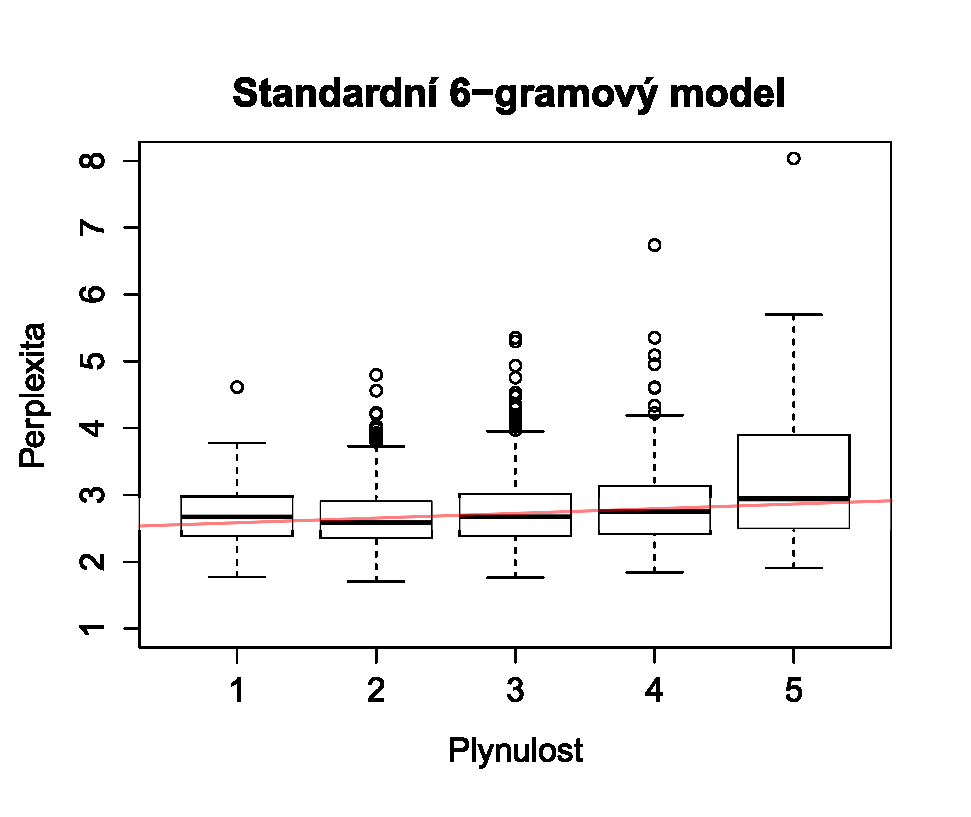
\includegraphics[width=60mm]{./grafy/morf/ngram/pad.svg.eps}
  \caption{Standardní 6-gramový model - pád}\label{gr:ngpad}
\endminipage\quad
\minipage{0.45\textwidth}
  \centering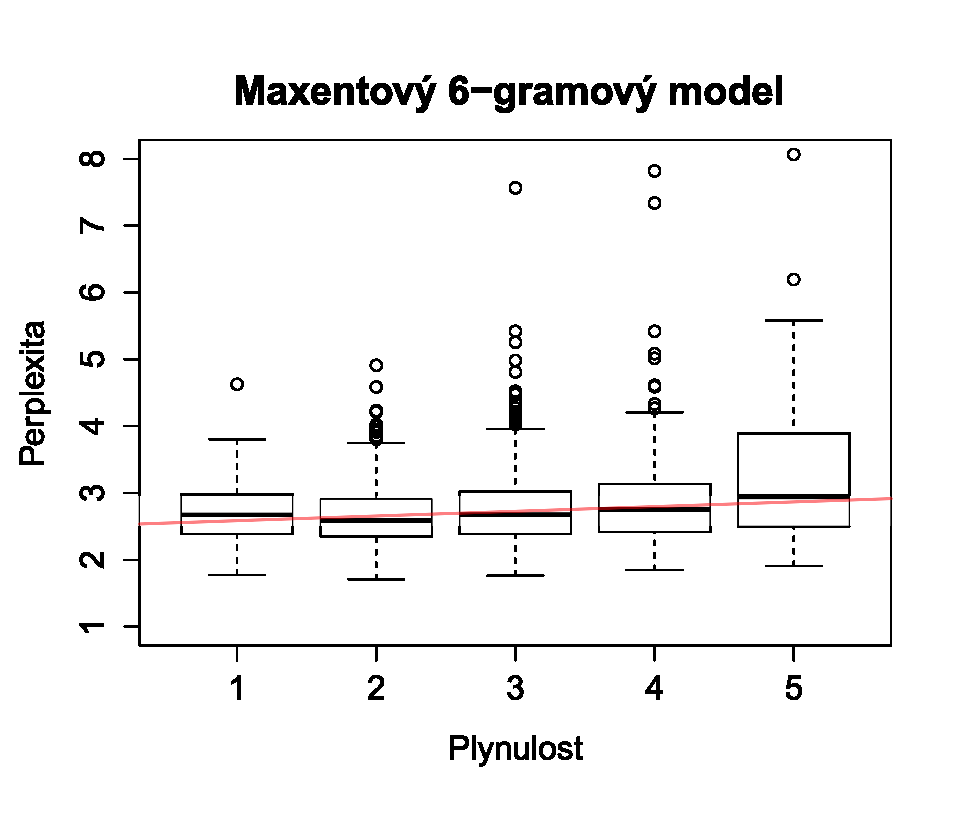
\includegraphics[width=60mm]{./grafy/morf/maxent/pad.svg.eps}	
  \caption{Maxentový 6-gramový - pád}\label{gr:maxpad}
\endminipage
\end{center}
\end{figure}

Výsledky opět nejsou dobré a jen potvrzují, že poskytnutí modelu značek pouze z jedné morfologické kategorie je nedostatečná informace.

\begin{figure}[!htbp]
\begin{center}
	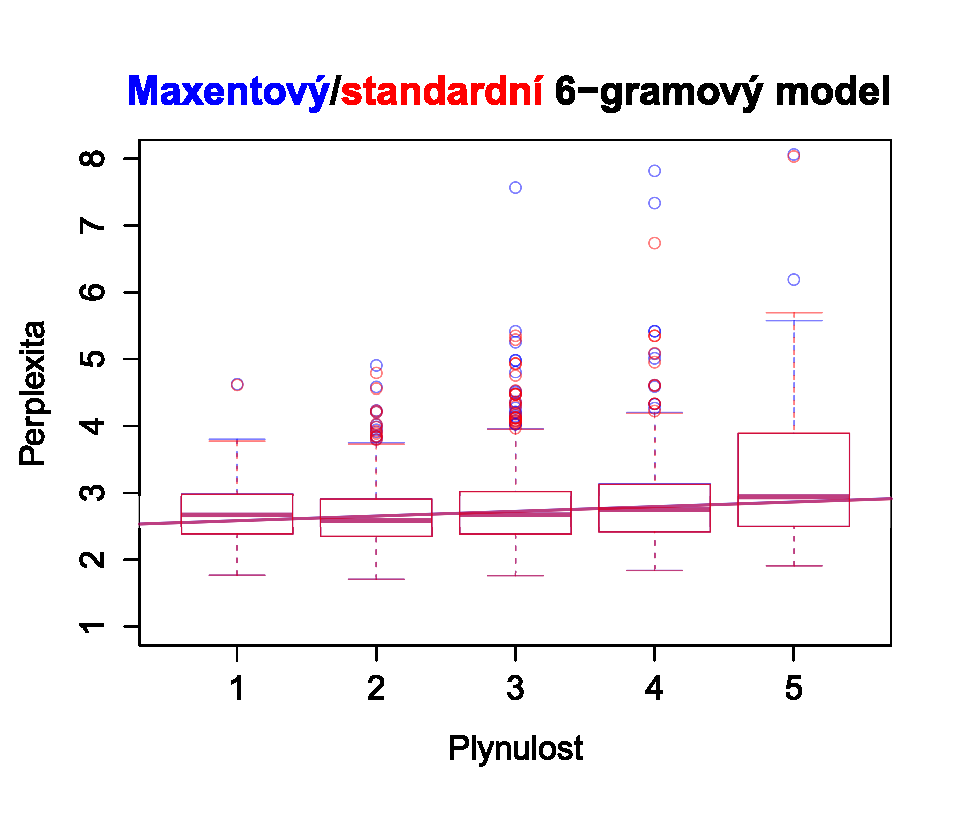
\includegraphics[width=90mm]{./grafy/morf/porovnani/pad.svg.eps}	
\end{center}
\caption{Porovnání modelů - pád}\label{gr:porpad}
\end{figure}

V porovnání jsou taktéž standardní n-gramové modely s modely maximálně entropie srovnatelné, bez větších rozdílů (obrázek \ref{gr:porpad}). Natrénování trvalo shodně 4 sekundy.


\subsection{S rozšířeným slovním druhem}
Jako v případech předchozích modelů se značkami z jedné morfologické kategorie, zkusíme přidat k pádu ještě rozšířený slovní druh.

\begin{figure}[!htb]
\begin{center}
\minipage{0.45\textwidth}
  \centering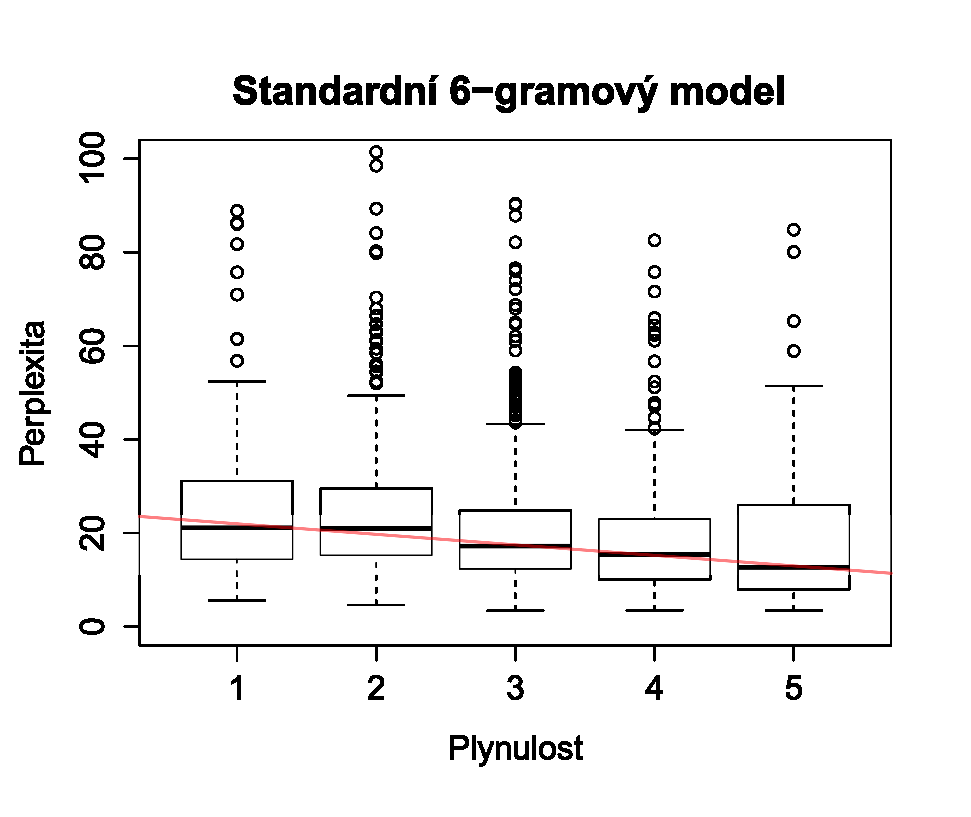
\includegraphics[width=60mm]{./grafy/morf/ngram/rsd+pad.svg.eps}
  \caption{Standardní 6-gramový model - rozšířený slovní druh + pád}\label{gr:ngrsd+pad}
\endminipage\quad
\minipage{0.45\textwidth}
  \centering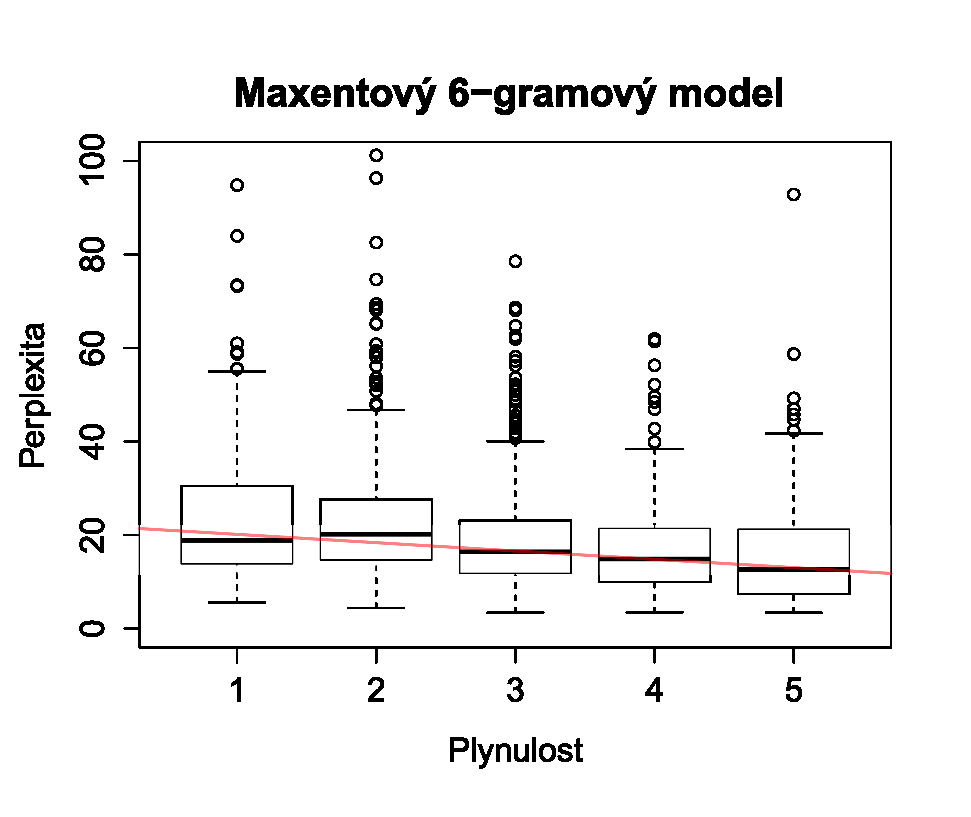
\includegraphics[width=60mm]{./grafy/morf/maxent/rsd+pad.svg.eps}
  \caption{Maxentový 6-gramový model - rozšířený slovní druh + pád}\label{gr:maxrsd+pad}
\endminipage
\end{center}
\end{figure}


\pagebreak



Zlepšení je znatelné a podobá se modelům s rozšířeným slovním druhem a všemi morfologickými značkami. Výsledky jsou prozatím nejlepší ze všech modelů se značkami jedné morfologické kategorie s rozšířeným slovním druhem.
\begin{figure}[!htbp]
\begin{center}
	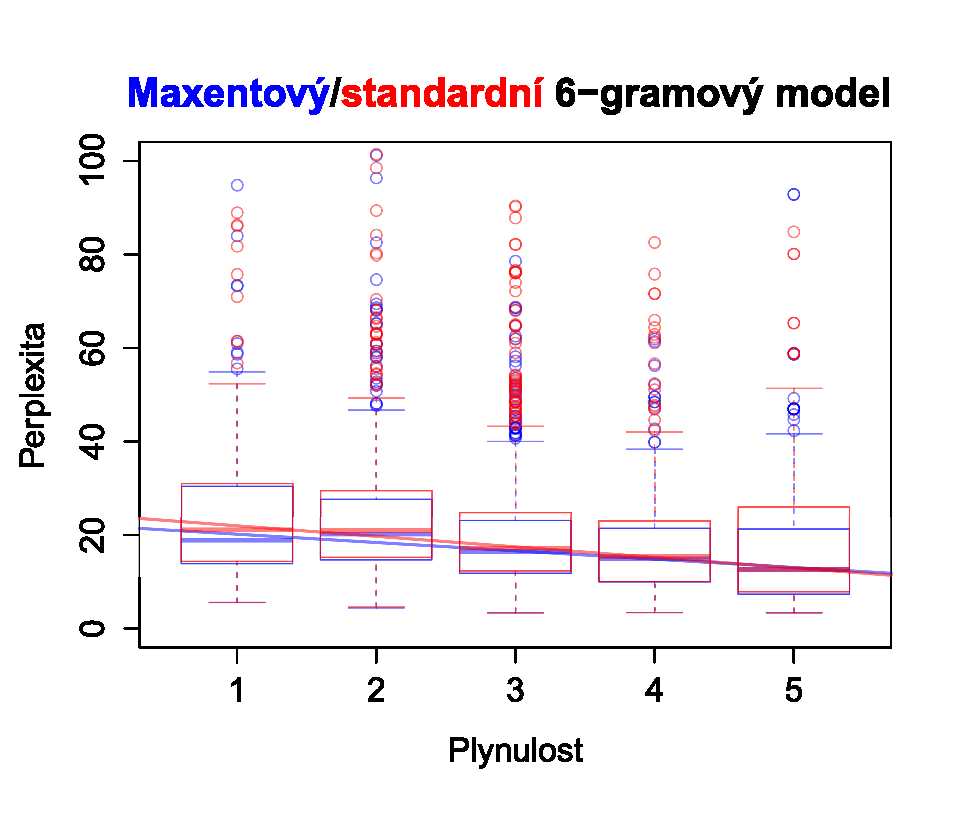
\includegraphics[width=90mm]{./grafy/morf/porovnani/rsd+pad.eps}
	\caption{Porovnání modelů - rozšířený slovní druh + pád}\label{gr:porrsd+pad}
\end{center}
\end{figure}


Maxentové modely dopadly o něco lépe a zvláště hypotézy hodnocené plynulostí 5 posunuly v perplexitě níže, což je správně. Nicméně proložená přímka je strmější u standardních n-gramů (obrázek \ref{gr:porrsd+pad}). Výpočetní nároky se ale výrazně liší - 34 sekund v případě standardních n-gramových modelů oproti 27 minutám v případě modelů maxentových.

\section{Shrnutí}
Zde uvedeme všechny naměřené hodnoty do tabulky. Tabulka bude obsahovat od každého modelu Pearsonův korelační koeficient\footnote{Udává vztah mezi dvěma veličinami. Nabývá hodnot $<-1, 1>$, přičemž 1 značí závislost přímou a -1 závislost nepřímou. Hodnota 0 indikuje, že vztah mezi veličinami nelze vyjádřit lineární funkcí.}, směrnici přímky proložené mediány boxplotů a čas potřebný k natrénování.


\pagebreak


\newcolumntype{M}[1]{>{\centering\arraybackslash}m{#1}}

\begin{table}[!htbp]
\begin{center}
\small\addtolength{\tabcolsep}{-3pt}
\begin{tabular}{|M{2.6cm}|M{1.4cm}|M{1.4cm}|M{1.4cm}|M{1.4cm}|M{1.4cm}|M{1.4cm}|}
\hline
\multirow{2}*{\textbf{Model}} & \multicolumn{2}{M{3.1cm}|}{\textbf{Pearsonův koeficient}} & \multicolumn{2}{M{3.1cm}|}{\textbf{Směrnice přímky}} & \multicolumn{2}{M{3.1cm}|}{\textbf{Čas trénování}} \\
\cline{2-7}
& {\tiny standardní} & {\tiny maxentový} & {\tiny standardní} & {\tiny maxentový} & {\tiny standardní} & {\tiny maxentový} \\
\hline
Slova & 0.05 & 0.05 & 33.53 & 17.43 & 3 min & 12 hod\\
\hline
RSD + všechny značky & -0.03 & 0.04 & -7.00 & -5.54 & 72 s & 8 hod s\\
\hline
RSD & 0.05 & 0.03 & -1.23 & -1.07 & 22 s & 14 min\\
\hline
Rod &  0.15 & 0.15 & 0.07 & 0.07 & 3 s & 4 s\\
\hline
Rod stejný s předchozím & 0.15 & 0.14 & 0.06 & 0.06 & 3 s & 3 s\\
\hline
RSD + rod & 0.04 & 0.03 & -1.42 & -1.41 & 36 s & 27 min\\
\hline
Číslo & 0.07 & 0.10 & 0.04 & 0.04 & 3 s & 3 s\\
\hline
Osoba + číslo & 0.06 & 0.09 & 0.07 & 0.07 & 4 s & 11 s\\
\hline
RSD + číslo & 0.03 & 0.02 & -1.70 & -1.70 & 33 s & 24 min\\
\hline
Pád & 0.15 & 0.15 & 0.07 & 0.07 & 4 s & 4 s\\
\hline
RSD + pád & 0.04 & 0.02 & -2.25 & -1.78 & 34 s & 27 min \\
\hline
\end{tabular}
\caption{Shrnutí výsledků modelů s morfologickými značkami}\label{tb:shrnutimorf}
\end{center}
\end{table}

U Pearsonova koeficientu bychom rádi dosáhli hodnoty blížící se k -1. Jedinou zápornou hodnotu má ale jen standardní n-gramový model natrénovaný na rozšířeném slovním druhu a všech morfologických značkách. Směrnice přímky by měla být záporná, aby přímka klesala. Čím menší bude, tím bude klesat strměji. Opět je hodnota nejnižší u standardního modelu se slovním druhem a všemi značkami (tabulka \ref{tb:shrnutimorf}).

Ačkoliv modely maximální entropie obvykle dostávaly nižší perplexitu než standardní modely, korelace perplexity a ručně hodnocené plynulosti vycházela lépe u standardních modelů. Trénování modelů maximální entropie trvalo ve většině případů mnohonásobně déle a nepřineslo pro naše experimenty žádné výrazné zlepšení.


\chapter{Modely s vlastní množinou rysů}
Problémy s německou gramatikou jsme se prozatím snažili řešit nahrazením slov morfologickými značkami. Modely s rozšířeným slovním druhem + morfologická analýza dopadly sice lépe než běžné modely trénované na slovech, přesto zlepšení není nijak výrazné. V následující kapitole se proto pokusíme upustit od n-gramů a postihnout gramatiku z jiné stránky - vlastní množinou rysů.

\section{Zdrojová data}

Pro následující experimenty používáme stejná data s ručně hodnocenou plynulostí jako v předchozí kapitole. Zde jsme je rozdělili na dva díly. Polovina tj. 1045 hodnocení překladových hypotéz se použije jako vývojová sada a druhá polovina jako sada testovací. Hypotézy byly rozděleny s ohledem na hodnocení plynulosti tak, aby vývojová i testovací množina vět obsahovala stejný počet hypotéz hodnocených plynulostí 1, 2, .., 5 (až na liché počty hypotéz některých plynulostí). Následující tabulka \ref{tb:rozdeleni} ukazuje přesné počty hypotéz a jejich rozdělení:

\begin{table}[!htbp]
\begin{center}\begin{tabular}{|c|c|c|c|}
	\hline
	\textbf{Plynulost} & \textbf{Celkem hypotéz} & \textbf{Vývojová sada} & \textbf{Testovací sada}\\
	\hline
	1 & 150 & 75 & 75\\
	\hline
	2 & 445 & 222 & 223\\
	\hline
	3 & 932 & 466 & 466\\
	\hline
	4 & 387 & 194 & 193\\
	\hline
	5 & 176 & 88 & 88\\
	\hline
	\hline	
	\multicolumn{1}{c}{\textbf{CELKEM}} & \multicolumn{1}{c}{\textbf{2090}} & \multicolumn{1}{c}{\textbf{1095}} & \multicolumn{1}{c}{\textbf{1095}}\\
\end{tabular}
\caption{Rozdělení hodnocení hypotéz na vývojová a testovací data}\label{tb:rozdeleni}
\end{center}\end{table}

Vzhledem k tomu, že budou rysy vycházet z německé gramatiky, budeme často potřebovat znát hranice klauzí dané věty. Určit klauze z hypotézy, která není gramaticky správně, je však obtížné - parser je v takovém případě zmatený a neudělá větný rozbor správně. Na základě toho používáme identifikované klauze z výchozího anglického textu, který je gramaticky správně, a na německé je pak převádíme pomocí zarovnání na úrovni slov. 

\section{Vlastní rysy}
Vlastní množina rysů sestává především z gramatických jevů, které n-gramy nemají možnost zachytit. Jedná se hlavně o tvorbu větného rámce. Mimo to ale budeme zkoumat, zda se ve větě třeba nevyskytuje více určitých sloves nebo naopak sloveso úplně chybí.

Celkem jsme sestavili 16 následujících rysů, u kterých vysvětlíme, jak fungují a co kontrolují, neboť ačkoliv jejich názvy intuitivně funkci napovídají, může být omezena jen na některé případy.
\begin{enumerate}
\item{\texttt{chybi\_infszu} - kontroluje, zda byla klauze uvozena spojkou vyžadující infinitiv s zu (rozšířený slovní druh \textit{KOUI}\footnote{ParZu používá pro označení rozšířeného slovního druhu Stuttgart/Tübinger Tagsets ZDROJ http://www.coli.uni-saarland.de/projects/sfb378/negra-corpus/stts.asc}), typicky se jedná o zkrácené vedlejší věty, a sleduje, zda ve větě takový infinitiv byl}
\item{\texttt{chybi\_podmet} - označuje skutečnost, že se v klauzi nevyskytlo slovo v prvním pádě}
\item{\texttt{chybi\_vfin} - v klauzi chybí určité sloveso}
\item{\texttt{chybi\_sum} - sčítá hodnoty všech rysů typu \texttt{chybi\_*}}
\item{\texttt{inf\_po\_vm\_neni\_na\_konci} - kontroluje, zda se za infinitivem po modálním slovese nevyskytlo ještě další slovo mimo sloves}
\item{\texttt{infszu\_neni\_na\_konci} - byla-li spojka vyžadující infinitiv s zu a zároveň se za infinitivem ještě vyskytlo další slovo mimo sloves}
\item{\texttt{vv\_sloveso\_neni\_na\_konci} - po podřadících spojkách (\textit{KOUS}, \textit{PRELS}, \textit{PRELAT}) kontroluje, zda po určitém slovesu nešlo ještě další slovo mimo sloves}
\item{\texttt{pp\_neni\_na\_konci} - pokud věta obsahovala pomocné sloveso, očekáváme příčestí minulé a kontrolujeme proto, zda se za ním ještě nevyskytlo další slovo mimo sloves}
\item{\texttt{neni\_na\_konci\_sum} - sčítá hodnoty všech rysů typu \texttt{*\_neni\_na\_konci}}
\item{\texttt{pp\_bez\_av} - bylo-li ve větě příčestí minulé bez pomocného slovesa a zároveň nebyla před příčestím minulým souřadící spojka, která by mohla oddělovat dvě věty se dvěma příčestími minulými, ale pomocným slovesem jen v první z nich (\textit{např.: Ich habe gekocht und gelernt.})}
\item{\texttt{neshoda\_podmet\_prisudek} - sledujeme výskyt prvního slova v nominativu nebo prvního slovesa, od těchto prvních výskytů si zapamatujeme číslo a osobu (u podstatných jmen ručně nastavíme, že se jedná o třetí osobu), pokud se nenajde shoda v čísle a osobě mezi prvním nalezeným nominativem a slovesem, pak daná klauze dostane tento rys}
\item{\texttt{vice\_osob} - funguje stejně jako předchozí, jenom s jiným vyhodnocením - tj. tehdy, když po první nalezené osobě nalezneme ještě další (samozřejmě v prvním pádě)}
\item{\texttt{vice\_vfin} - indikuje výskyt více určitých sloves v jedné klauzi}
\item{\texttt{vice\_sum} - sčítá hodnoty všech rysů typu \texttt{vice\_*}}
\item{\texttt{root} - projde větný rozbor z výstupu ParZu a spočítá počet kořenů, je-li totiž věta gramaticky správně, nalezneme kořen pouze jeden, v opačném případě je jich více a představují pomyslný počet chyb ve větě}
\item{\texttt{sum} - sčítá hodnoty všech předchozích rysů včetně rysu \texttt{root}}
\end{enumerate}

Pomocí programu Chyby, který vzniknul k této práci, jsme změřili na vývojových datech korelaci každého rysu s ručně hodnocenou plynulostí. Každý rys kromě rysů součtových a rysu \texttt{root} jsou určovány pro každou klauzi zvlášť a mohou v ní vždy dostat jen hodnotu \texttt{true}/\texttt{false}. Rysy celé věty jsou pak součtem hodnot rysů ze všech klauzí - přičteme vždy jedničku, když daný rys nabyl v klauzi hodnoty \texttt{true}.

\subsection{Rysy typu chybi\_*}
\begin{figure}[!htb]
\minipage{0.31\textwidth}
  \centering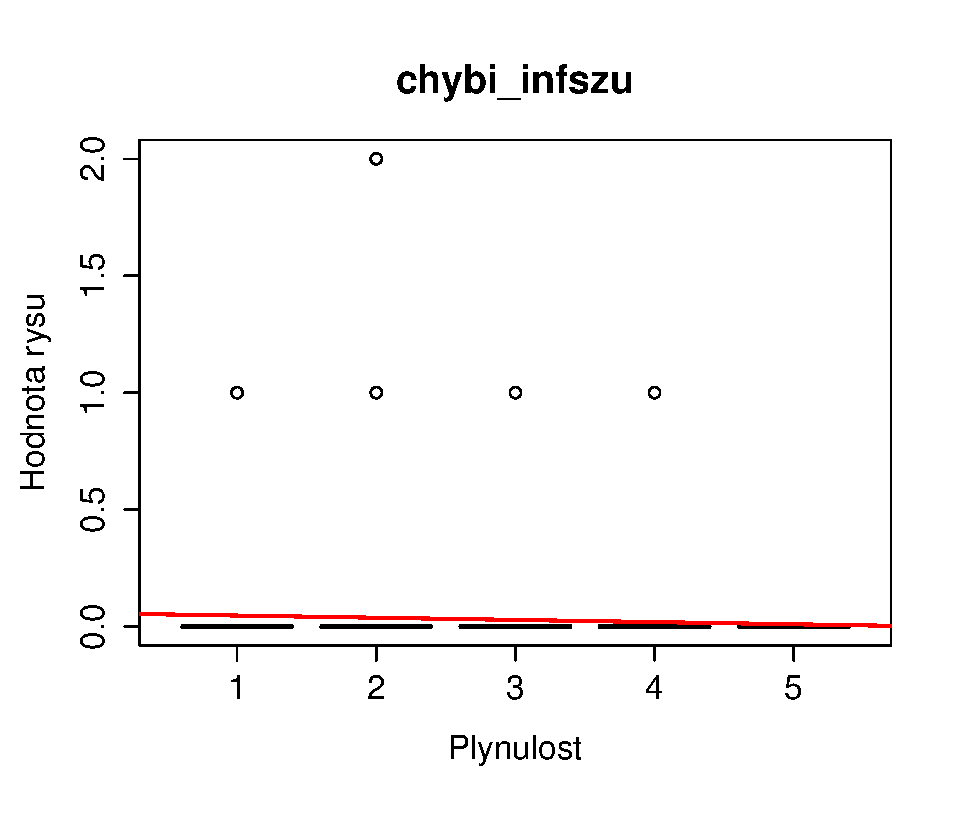
\includegraphics[width=50mm]{./grafy/rysy/chybi_infszu.eps}
  \caption{Korelace hodnoty rysu chybi\_infszu a plynulosti}\label{gr:infszu}
\endminipage\hfill
\minipage{0.31\textwidth}
  \centering\includegraphics[width=50mm]{./grafy/rysy/chybi_podmet.eps}
  \caption{Korelace hodnoty rysu chybi\_podmet a plynulosti}\label{gr:podmet}
\endminipage\hfill
\minipage{0.31\textwidth}
  \centering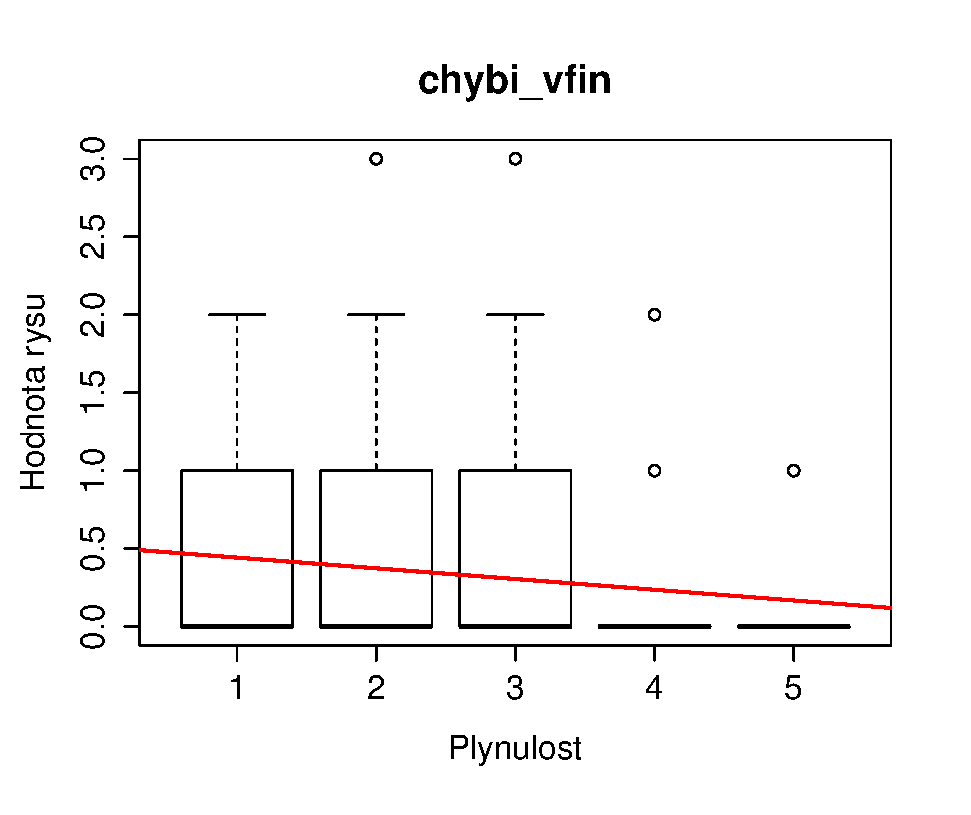
\includegraphics[width=50mm]{./grafy/rysy/chybi_vfin.eps}
  \caption{Korelace hodnoty rysu chybi\_vfin a plynulosti}\label{gr:vfin}
\endminipage\hfill
\end{figure}

\begin{figure}[!htb]
\centering\minipage{0.31\textwidth}
  \centering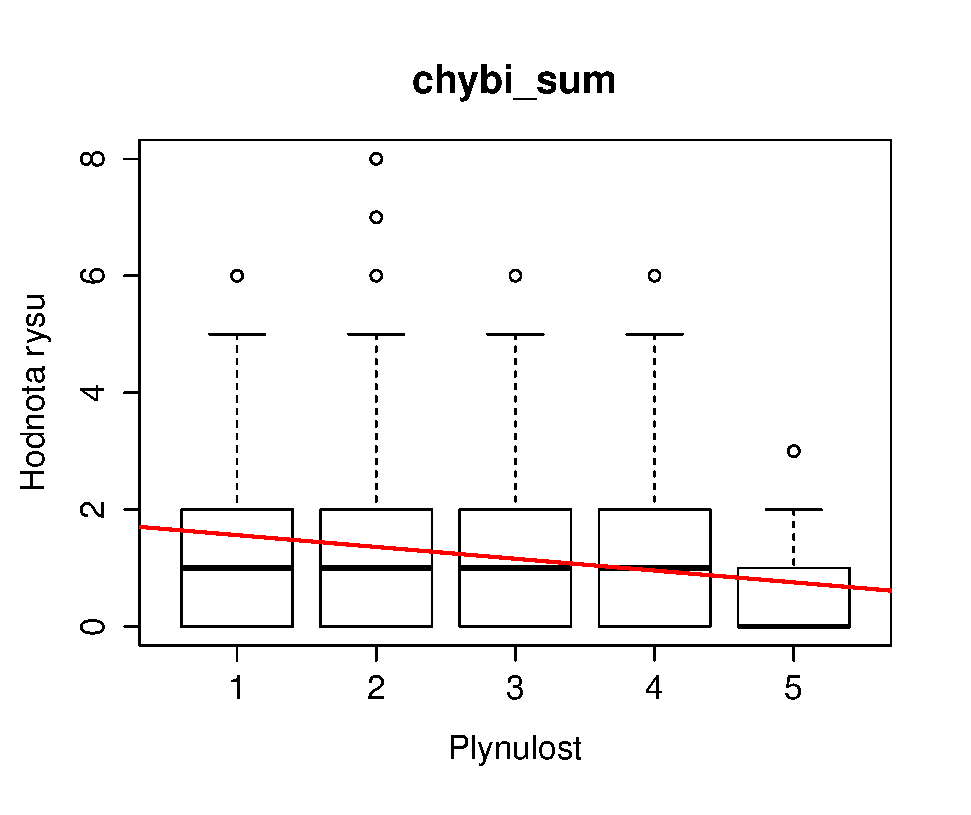
\includegraphics[width=50mm]{./grafy/rysy/chybi_sum.eps}
  \caption{Korelace součtového rysu chybi\_sum a plynulosti}\label{gr:chybi}
\endminipage
\end{figure}

Jednotlivé rysy samostatně neukázaly závislost s plynulostí (obrázky \ref{gr:infszu}, \ref{gr:podmet}, \ref{gr:vfin}). V součtu je u hypotéz s plynulostí 5 medián na nule, což je správně, neboť tyto hypotézy by měly být úplně bez chyb (obrázek \ref{gr:chybi}). Hodnoty nad nulou jsou způsobené jednak díky chybám v hranicích klauzí, protože se v nich spoléháme na identifikaci klauzí anglických a na zarovnání slov. Jednak také díky chybám při morfologické analýze z ParZu a samozřejmě také díky speciálním případům, se kterými náš program na vyhledávání hodnot rysů, nepočítá.

\pagebreak


\subsection{Rysy typu *\_neni\_na\_konci}
\begin{figure}[!htb]
\minipage{0.31\textwidth}
  \centering\includegraphics[width=50mm]{./grafy/rysy/inf_po_vm_neni_na_konci.eps}
  \caption{Korelace hodnoty rysu inf\_po\_vm\_neni\_na\_konci a plynulosti}\label{gr:vm}
\endminipage\hfill
\minipage{0.31\textwidth}
  \centering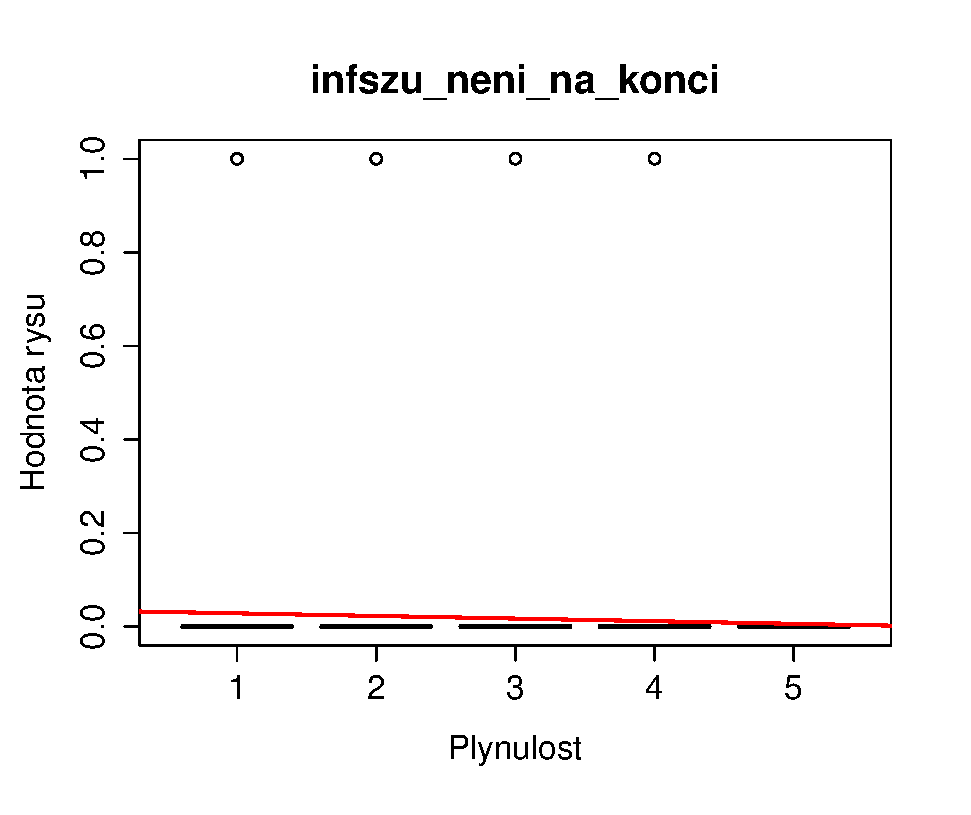
\includegraphics[width=50mm]{./grafy/rysy/infszu_neni_na_konci.eps}
  \caption{Korelace hodnoty rysu infszu\_neni\_na\_konci a plynulosti}\label{gr:infszu_konec}
\endminipage\hfill
\minipage{0.31\textwidth}
  \centering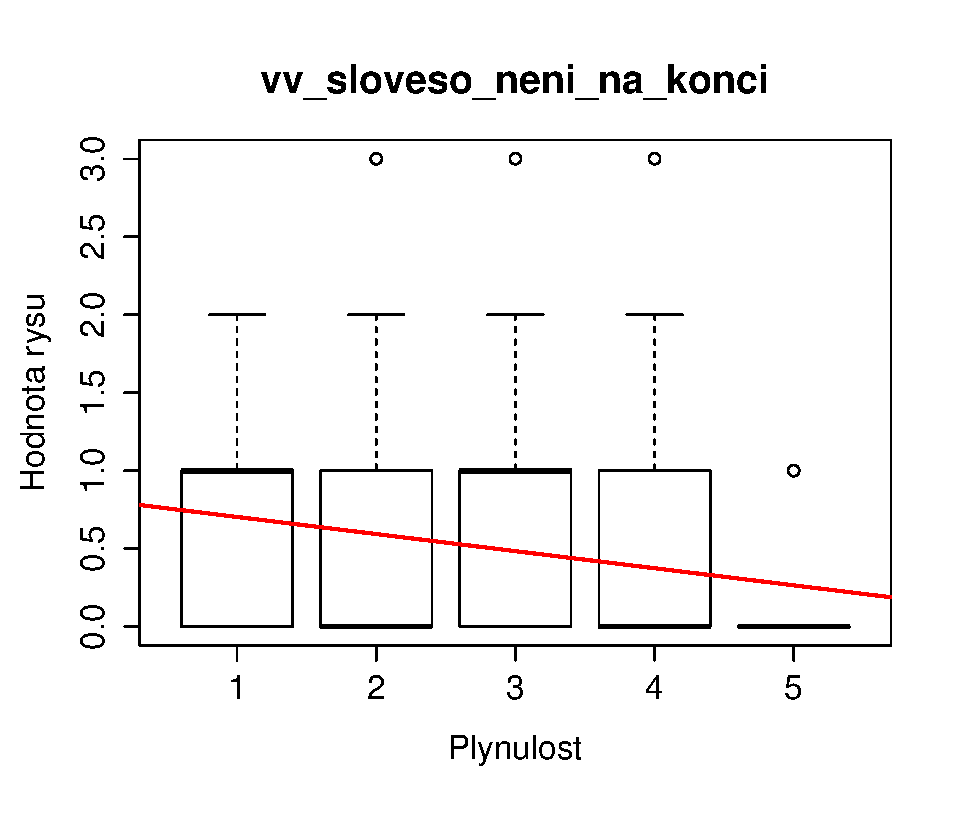
\includegraphics[width=50mm]{./grafy/rysy/vv_sloveso_neni_na_konci.eps}
  \caption{Korelace hodnoty rysu vv\_sloveso\_neni\_na\_konci a plynulosti}\label{gr:vvsloveso}
\endminipage\hfill
\end{figure}


\begin{figure}[!htb]
\begin{center}
\minipage{0.31\textwidth}
  \centering\includegraphics[width=50mm]{./grafy/rysy/pp_neni_na_konci.eps}
  \caption{Korelace hodnoty rysu pp\_neni\_na\_konci a plynulosti}\label{gr:pp_konec}
\endminipage\quad
\minipage{0.31\textwidth} 
  \centering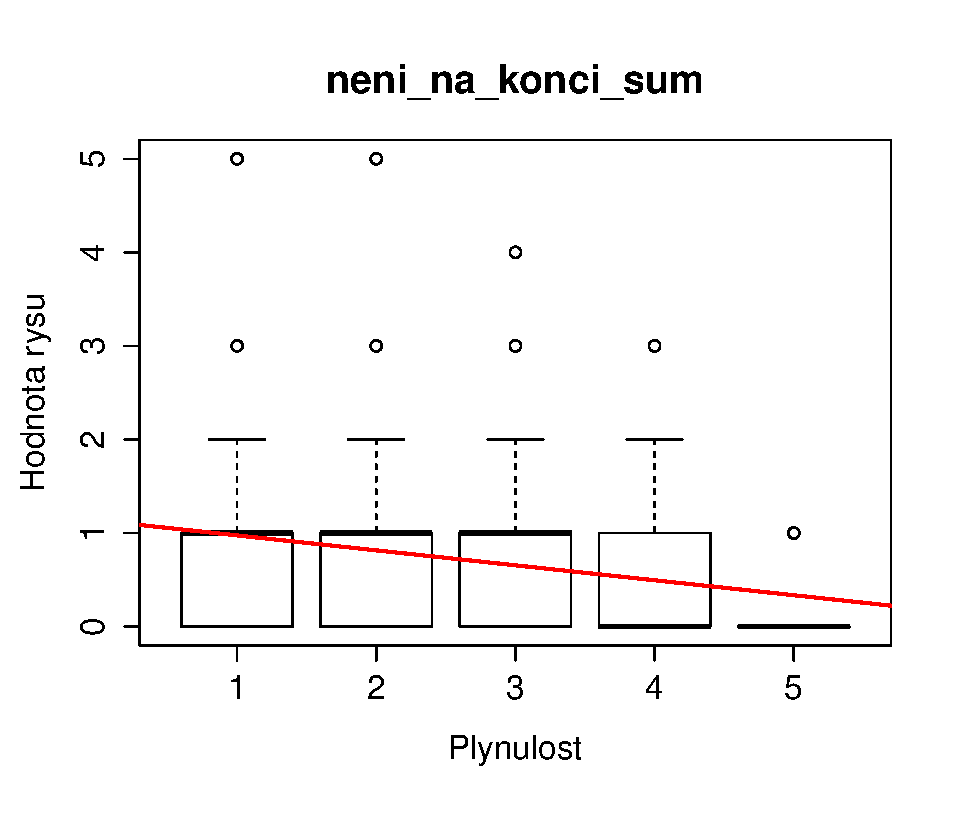
\includegraphics[width=50mm]{./grafy/rysy/neni_na_konci_sum.eps}
  \caption{Korelace součtového rysu neni\_na\_konci\_sum a plynulosti}\label{gr:sumneni}
\endminipage
\end{center}
\end{figure}


Zde je situace podobná jako u předchozí skupiny rysů. Jednotlivé rysy samostatně (obrázky \ref{gr:vm}, \ref{gr:infszu_konec}, \ref{gr:vvsloveso}, \ref{gr:pp_konec}) mají mediány na nule. U součtového rysu (obrázek \ref{gr:sumneni}) alespoň hypotézy s hodnocením plynulosti 5 dostávaly oproti ostatním plynulostem častěji nulu.


\subsection{Rysy pp\_bez\_av a neshoda\_podmet\_prisudek}
\begin{figure}[!htb]
\begin{center}
\minipage{0.31\textwidth}
  \centering\includegraphics[width=50mm]{./grafy/rysy/pp_bez_av.eps}
  \caption{Korelace hodnoty rysu pp\_bez\_av a plynulosti}\label{gr:bezav}
\endminipage\quad
\minipage{0.31\textwidth}
  \centering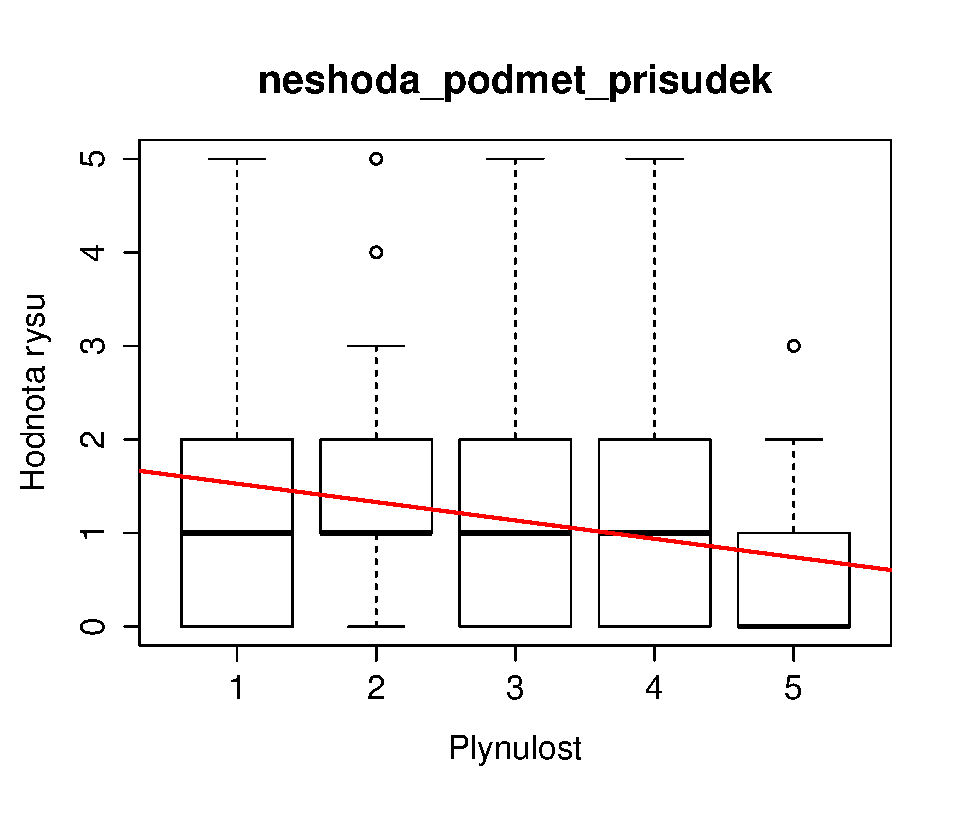
\includegraphics[width=50mm]{./grafy/rysy/neshoda_podmet_prisudek.eps}
  \caption{Korelace hodnoty rysu neshoda\_podmet\_prisudek a plynulosti}\label{gr:neshoda}
\endminipage
\end{center}
\end{figure}

Oba rysy opět nevykazují samostatně souvislost s plynulostí (obrázky \ref{gr:bezav}, \ref{gr:neshoda}). 


\subsection{Rysy typu vice\_*}

\begin{figure}[!htb]
\minipage{0.31\textwidth}
  \centering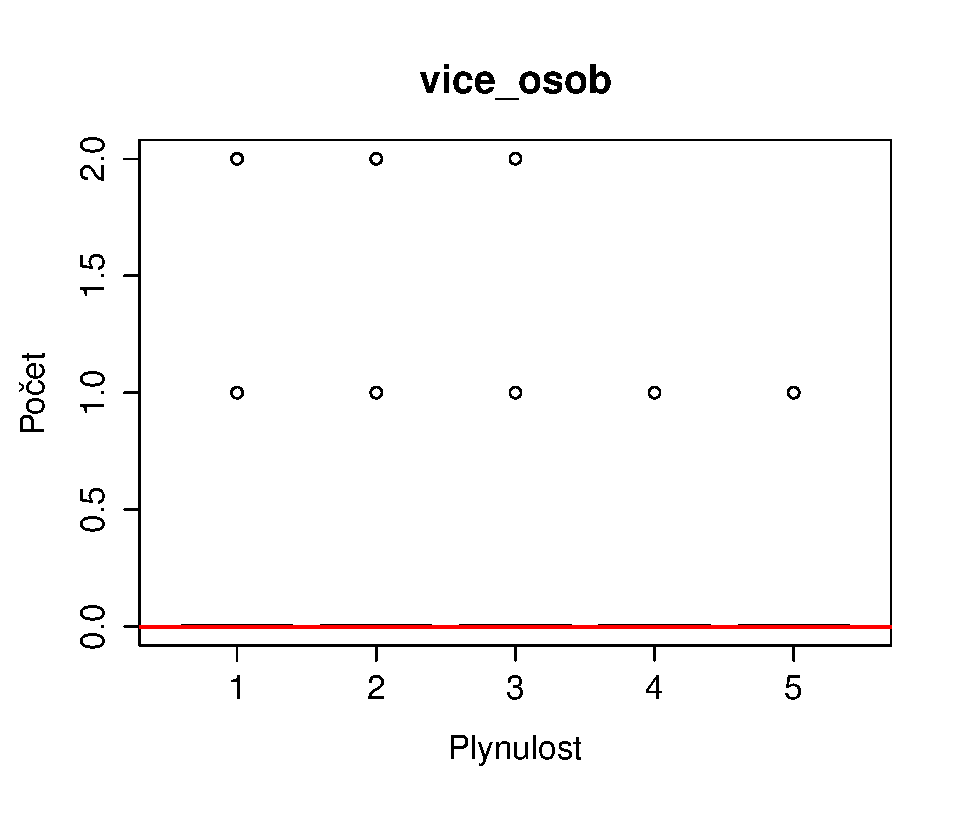
\includegraphics[width=50mm]{./grafy/rysy/vice_osob.eps}
  \caption{Korelace hodnoty rysu vice\_osob a plynulosti}\label{gr:viceosob}
\endminipage\hfill
\minipage{0.31\textwidth}
  \centering\includegraphics[width=50mm]{./grafy/rysy/vice_vfin.eps}
  \caption{Korelace hodnoty rysu vice\_vfin a plynulosti}\label{gr:vicevfin}
\endminipage\hfill
\minipage{0.31\textwidth}
  \centering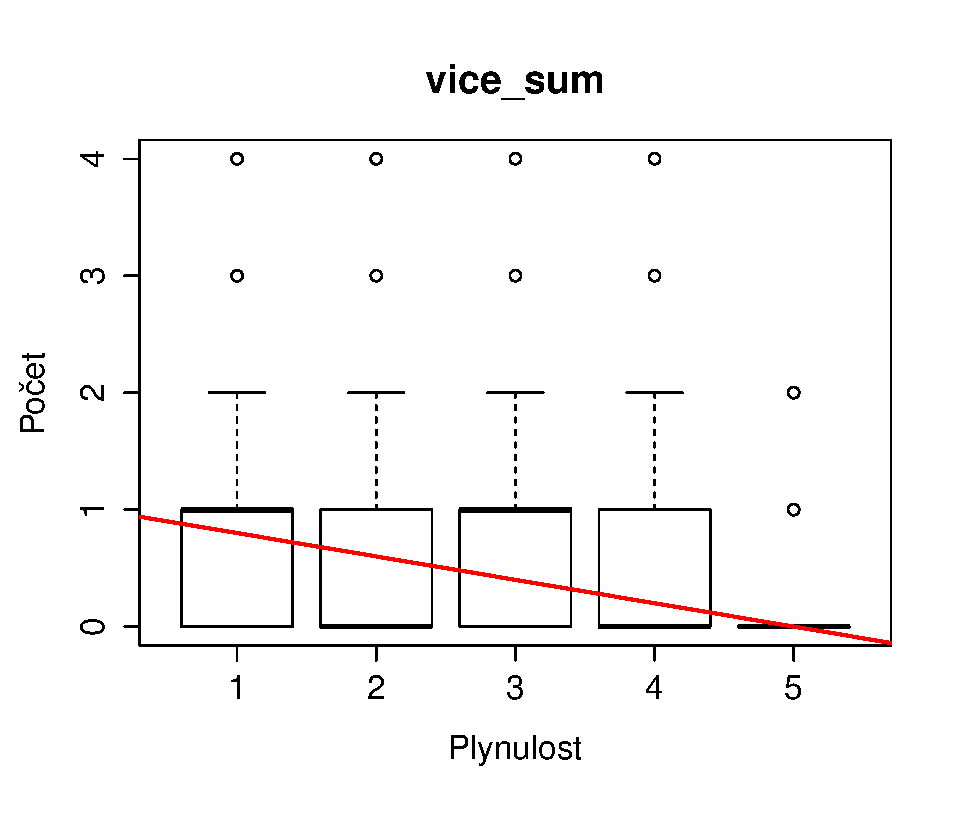
\includegraphics[width=50mm]{./grafy/rysy/vice_sum.eps}
  \caption{Korelace součtového rysu vice\_sum a plynulosti}\label{gr:vicesum}
\endminipage\hfill
\end{figure}

Shodně dopadly i rysy typu \texttt{vice\_*}. Mediány rysu \texttt{vice\_osob} jsou nulové (obrázek \ref{gr:viceosob}). U rysu \texttt{vice\_vfin} mediány kolísají mezi nulou a jedničkou (obrázek \ref{gr:vicevfin}), stejně jako i u součtového rysu (obrázek \ref{gr:vicesum}).

\subsection{Rysy sum a root}
\begin{figure}[!htb]
\begin{center}
\minipage{0.31\textwidth}
  \centering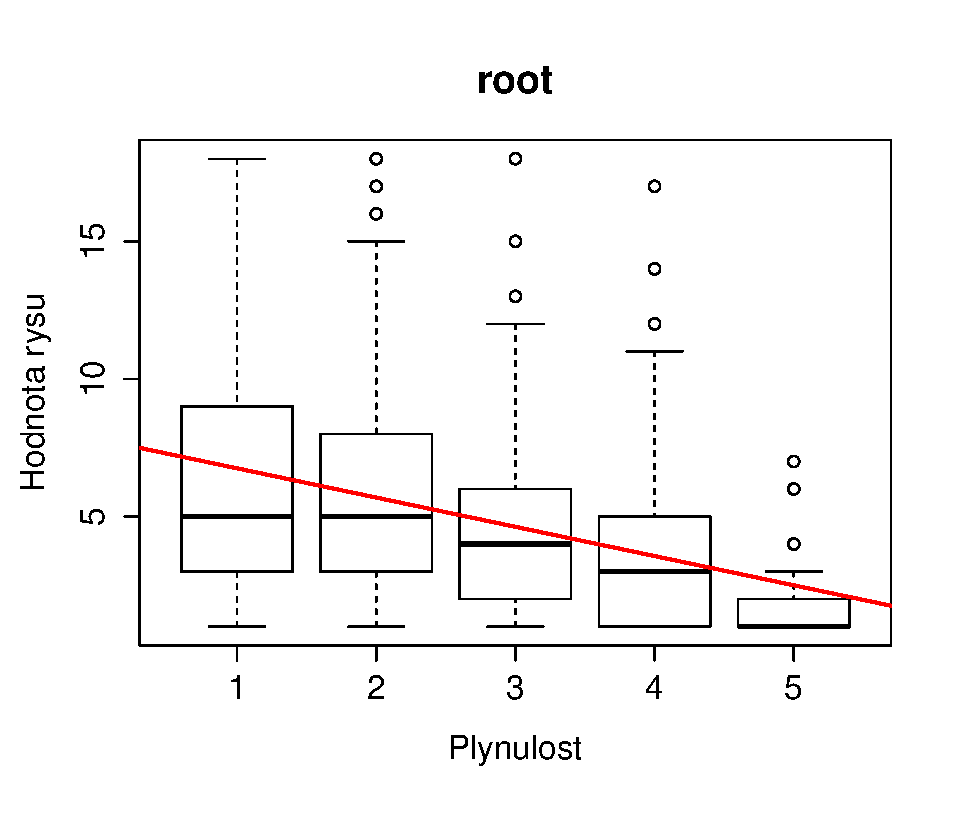
\includegraphics[width=50mm]{./grafy/rysy/root.eps}
  \caption{Korelace hodnoty rysu root a plynulosti}\label{gr:root}
\endminipage\quad
\minipage{0.31\textwidth}
  \centering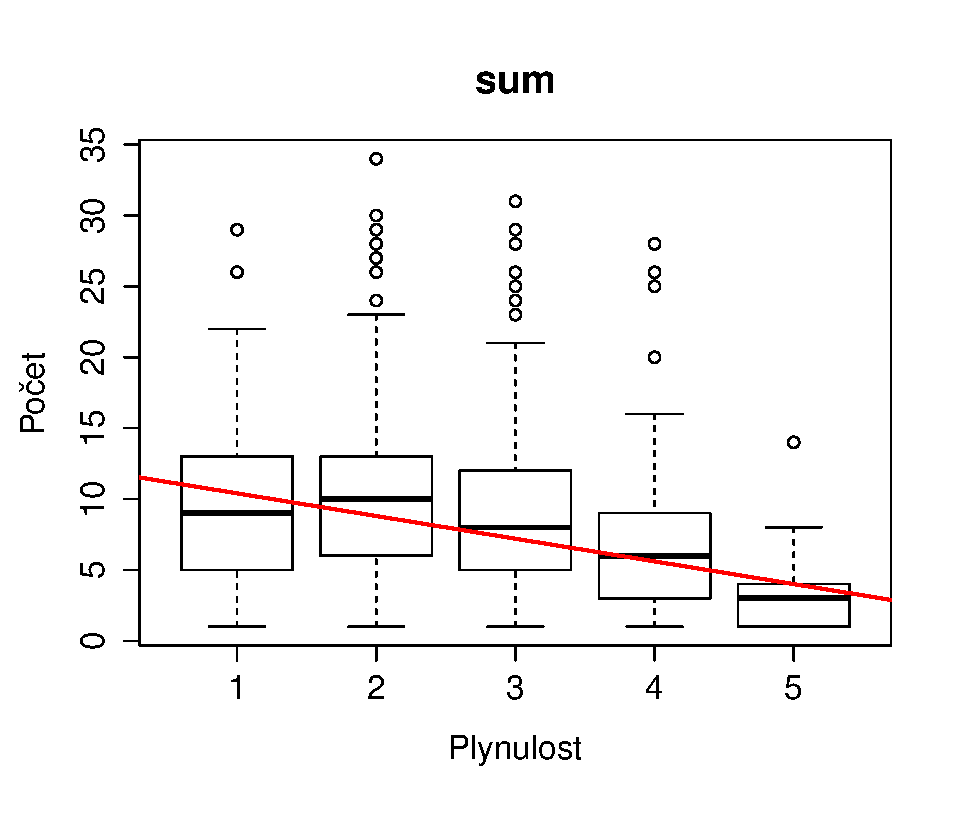
\includegraphics[width=50mm]{./grafy/rysy/sum.eps}
  \caption{Korelace hodnoty rysu sum a plynulosti}\label{gr:sum}
\endminipage
\end{center}
\end{figure}

Oba rysy vykazují závislost jejich hodnot s plynulostí (obrázky \ref{gr:root}, \ref{gr:sum}). Mediány mají pro různé plynulosti odlišné hodnoty (až na plynulosti 4 a 5). V následujících experimentech proto zkusíme, zda se dá predikovat plynulost třeba jen na základě mediánu vypočteného pro jednotlivé plynulosti v trénovacích datech.


\subsection{Přesnost určení rysů}
Jak jsme již zmínili, určování rysů se musí spoléhat na další výstupy nástrojů, které taktéž nepracují bezchybně. Abychom alespoň orientačně věděli, jak přesné určení rysů je, analyzovali jsme ručně 15 náhodných vět a kontrolovali, zda se hodnota rysu shoduje se skutečností. V rámci ruční kontroly jsme přišli na to, že spoustu chyb v určení zapříčiňuje špatná identifikace slovního druhu parserem ParZu. K chybě dochází především z důvodu, že německé hypotézy jsou psané pouze malými písmeny. V němčině ale často právě velké písmeno rozhodne o tom, zda se jedná o sloveso nebo podstatné jméno, \textit{např. zahlen x Zahlen}.


Příklad ruční analýzy:

\textit{in vielen ländern , aber die politischen parteien sich schwer vorstellen , daß solche debatten auch .}
\begin{center}
\begin{tabular}{>{\small\texttt}l>{\small\texttt}l|>{\small\texttt}l>{\small\texttt}l}
ok	&chybi\_infszu:0 &
-1	&chybi\_podmet:1\\
	&chybi\_sum:1 &
+1	&chybi\_vfin:0\\
ok	&inf\_po\_vm\_neni\_na\_konci:0 &
ok	&infszu\_neni\_na\_konci:0\\
	&neni\_na\_konci\_sum:0 &
ok	&neshoda\_podmet\_prisudek:1\\
ok	&pp\_bez\_av:0 &
ok	&pp\_neni\_na\_konci:0\\
	&root:3 &
	&sum:5\\
ok	&vice\_osob:0 &
	&vice\_sum:0\\
ok	&vice\_vfin:0 &
ok	&vv\_sloveso\_neni\_na\_konci:0\\
\end{tabular}
\end{center}

Ve sloupci nalevo od názvu rysu je uvedeno stanovisko - ok označuje souhlas, kladná hodnota udává, o kolik měla být hodnota rysu vyšší, záporná udává opak tj. o kolik měla být hodnota nižší. Součtové rysy hodnoceny nebyly, neboť vychází z ostatních. Stejně jako rys \texttt{root} nebyl hodnocen, neboť ten stanovujeme pouze na základě výstupu z ParZu.

Stanovení, zda je některý rys správně či špatně, je někdy sporné, neboť mnoho hypotéz nedává smysl a spoustu věcí tak musíme jen odhadovat. V této hypotéze například nevíme, zda se jedná o dvě nebo tři klauze, proto jsme rys \texttt{chybi\_vfin} mohli ohodnotit jako +1 nebo +2. Zde jsme zvolili +1, pokud bychom ohodnotili jako +2, pak bychom zase u \texttt{chybi\_podmet} museli namísto -1 zvolit ok.

Vyhodnocení jsme potom stanovili jako součet hodnot rysů, jaké byly stanoveny programem, a součet hodnot, jaké měly být ve skutečnosti. Podílem jsme potom získali číslo okolo 53 \%. Toto číslo ale udává jen úspěšnost rysů, které nabyly hodnoty vyšší než nula. Abychom zohlednili i rysy, které měly být hodnocené nulou a nulu dostaly, zvýšíme všem rysům hodnocení o jedna. Hodnoty znovu sečteme a vydělíme. Výpočet udává necelých 87 \%.

\section{Princip experimentů}

Princip experimentů bude následující:
\begin{itemize}
\item{identifikovat německé klauze v hypotézách na základě anglických s využitím zarovnání na úrovni slov}
\item{provést morfologickou analýzu a pokusit se o větný rozbor hypotéz}
\item{pokusit se vyhledat některé gramatické chyby a použít je jako rysy}
\item{natrénovat maxentový a mediánový\footnote{Mediánovým modelem rozumíme model pro náš klasifikátor hodnotící jen na základě mediánů} model s těmito rysy}
\item{provést stejný postup na testovacích datech a model otestovat}
\end{itemize}

Pro identifikaci klauzí vzniknul k bakalářské práci program Klauze, který na základě anglických klauzí a zarovnání na úrovni slov identifikuje klauze německé a vydá na výstup jejich hranice. Ze zarovnání bereme jen ty nejvíce jisté shody (int?), neboť nám nejde o kompletní zarovnání, ale jen o hranice klauzí. Na základě anglických klauzí jsou nejdříve slova roztříděna podle zarovnání do klauzí. Slova v klauzích se potom setřídí podle pořadí, v jakém byly v hypotéze. Poté se dle minimálního a maximálního indexu slova (počítáno zleva od nuly) rozhoduje, zda se jedná o větu vloženou nebo zda má začínat až pozdějším slovem, neboť se kryje s větou předchozí. Tímto způsobem se určí hranice klauzí tak, aby zahrnuly všechny slova ve větě.

Na morfologickou analýzu a větný rozbor použijeme opět parser ParZu. Tentokrát ale využijeme ještě dalších informací, které poskytuje. Zkusíme využít v náš prospěch i skutečnosti, že u gramaticky špatné věty postaví větný rozbor chybně.

Pro hledání chyb v jednotlivých klauzích jsme stvořili program Chyby. Ten se na základě provedené analýzy z ParZu a hranicí klauzí snaží určit některé gramatické chyby, pro celou větu pak vydá tyto chyby jako součet všech klauzí. Výstupem je soubor ve formátu ihned použitelném pro natrénování v Maxent Toolkitu od Le Zhanga. Za pomocí rysů vycházejících z gramatiky se budeme snažit predikovat plynulost. Výstupní formát bude tedy např. následující:

\begin{center}
\begin{tabular}{llll}
\hline
\texttt{1} & \texttt{chybi\_vfin:2} & \texttt{pp\_bez\_av:3} & \texttt{chybi\_infszu:1} \\
\texttt{4} & \texttt{chybi\_vfin:0} & \texttt{pp\_bez\_av:0} & \texttt{chybi\_infszu:1} \\
\texttt{2} & \texttt{chybi\_vfin:1} & \texttt{pp\_bez\_av:2} & \texttt{chybi\_infszu:0} \\
\hline
\end{tabular}
\end{center}

Jak vidíme z příkladu, druhý řádek nám říká, že hypotéza hodnocená plynulostí 4 má hodnotu rysu \texttt{chybi\_vfin} 0, \texttt{pp\_bez\_av} 0 a \texttt{chybi\_infszu} 1.

Maxentové modely budeme trénovat v MaxentToolkitu(ZDROJ) od Le Zhanga. Pro určení vah rysů využijeme výchozího nastavení tj. metody LBFGS.

V úvodním seznamu kroků této sekce jsme se zmínili o mediánovém modelu. U korelací rysů root a sum jsme zmínili, že zkusíme, zda lze plynulost predikovat jen na základě mediánů jednotlivých plynulostí. Za tímto účelem jsme vytvořili vlastní takový klasifikátor. Z trénovacích dat si vypočítá pro každý rys a každou plynulost medián. Souhrn mediánů je pak zapsán jako model. Při testování vycházíme z těchto mediánů - každý rys vydá jeden návrh plynulosti, tyto návrhy zprůměrujeme a dostaneme výslednou navrhovanou plynulost. Pokud jsou mediány dvou plynulostí stejné, zvýšíme ten, který patří horší plynulosti, o jedna. Vstupní formát je shodný s formátem pro maxentové modely.

\section{Způsob vyhodnocení}
U obou typů modelů budeme vyhodnocovat hlavně přesnost predikce tj. procentuálně vyjádříme, v kolika případech se model trefil do správné plynulosti. Mimo to budeme ještě zkoumat, v kolika případech se plynulost navrhovaná modelem lišila od skutečnosti jen o 1. Abychom ale mohli brát tento údaj v potaz, vypíšeme vždy ještě počty jednotlivých plynulostí, které model nabídnul. Pokud bychom tyto počty nezohlednili, mohlo by se stát, že model bude slepě tipovat vždy plynulost 3, kterých je nejvíce (44.6 \%). Potom by lišící se o jedna byly hypotézy s plynulostí 2 a 4, kterých je dohromady 38 \%. Dopředu proto stanovíme, že údaj, kdy se navrhovaná plynulost od skutečnosti lišila jen o jedna, budeme brát v potaz pouze za předpokladu, že model nabídnul každou plynulost alespoň jednou. 


\section{Modely se všemi rysy}
Jako první zkusíme natrénovat modely se všemi šestnácti rysy.

\begin{table}[!htbp]
\begin{center}
\begin{tabular}{|r|c|c|}
\hline
 & \textbf{Maxentový model} & \textbf{Mediánový model} \\
 \hline
přesnost & 41.24 \%  & 28.23 \%  \\
\hline
lišící se o 1 & 38.85 \% & 47.94 \%  \\
\hline
\textbf{počty} \quad 1 & \color{red}0 & \color{red}0 \\
\textbf{plynulostí} \quad 2 & 278 & \color{red}0 \\
 3 & 767 & 245 \\
 4 & \color{red}0 & 727 \\
 5 & \color{red}0 & 73 \\
\hline
\end{tabular}
\caption{Naměřené hodnoty modelů se všemi rysy}\label{tb:all}
\end{center}
\end{table}

Přesnost obou modelů je nižší než, kdybychom slepě tipovali samé trojky (44.6 \% - tuto hodnotu budeme dále označovat jako baseline). Ani jeden z modelů nenabídnul od každou plynulost alespoň jednou, a proto dle stanoveného kritéria, nebereme údaje lišící se o 1 jako relevantní (tabulka \ref{tb:all}.


\section{Modely se součtovými rysy}
Při znázorňování korelace rysů a plynulosti vždy vyšly o něco lépe součtové rysy. Konkrétně se jedná o rysy chybi\_sum, neni\_na\_konci\_sum, sum, vice\_sum. Zkusíme proto modely natrénovat právě jenom na nich. 

\begin{table}[!htbp]
\begin{center}
\begin{tabular}{|r|c|c|}
\hline
 & \textbf{Maxentový model} & \textbf{Mediánový model} \\
 \hline
     přesnost & 42.58 \%  & 32.15 \%  \\
\hline
lišící se o 1 & 39.23 \% & 46.70 \%  \\
\hline
     \textbf{počty} \quad 1 & \color{red}0   & \color{OliveGreen}6   \\
\textbf{plynulostí} \quad 2 & 128 & \color{OliveGreen}104   \\
                          3 & 917 & \color{OliveGreen}329 \\
                          4 & \color{red}0   & \color{OliveGreen}464 \\
                          5 & \color{red}0   & \color{OliveGreen}142  \\
\hline
\end{tabular}
\caption{Naměřené hodnoty modelů se všemi součtovými rysy}\label{tb:allsums}
\end{center}
\end{table}

Maxentový model se dotýká hranice baseline, bohužel ji ale nepřekonává. Mediánový model je na tom s přesností hůře, ovšem nabídnul každou plynulost alespoň jednou. Můžeme proto u něj brát i v potaz, že počet hypotéz, kdy se lišil o jedna, je 46.70 \% (tabulka \ref{tb:allsums}.

\subsection{S rysem root}
Mimo součtové rysy, co se korelace týče, dopadnul dobře i rys root. Zkusíme jej proto přidat k součtovým rysům.

\begin{table}[!htbp]
\begin{center}
\begin{tabular}{|r|c|c|}
\hline
 & \textbf{Maxentový model} & \textbf{Mediánový model} \\
 \hline
     přesnost & 40.67 \%  & 32.97 \%  \\
\hline
lišící se o 1 & 40.10 \% & 49.00 \%  \\
\hline
     \textbf{počty} \quad 1 & \color{red}0   & \color{OliveGreen}11   \\
\textbf{plynulostí} \quad 2 & 205 & \color{OliveGreen}227   \\
                          3 & 840 & \color{OliveGreen}301 \\
                          4 & \color{red}0   & \color{OliveGreen}415 \\
                          5 & \color{red}0   & \color{OliveGreen}91  \\
\hline
\end{tabular}
\caption{Naměřené hodnoty modelů se součtovými rysy a rysem root}\label{tb:allsumsroot}
\end{center}
\end{table}

Toto přidání se ale projevilo negativně u maxentových modelů a jen o 0.82 \% si polepšil mediánový model v přesnosti. Znovu ale nabídnul všechny hodnoty plynulosti. V počtu lišících se o 1 si polepšil o 2.3 \% (tabulka \ref{tb:allsumsroot}).


\section{Modely s rysem root}
Rys root vypadal v korelaci s plynulostí slibně. Se součtovými rysy přílišné zlepšení nepřinesl, zkusíme jej proto použít zcela samostatně.

\begin{table}[!htbp]
\begin{center}
\begin{tabular}{|r|c|c|}
\hline
 & \textbf{Maxentový model} & \textbf{Mediánový model} \\
 \hline
     přesnost & 44.60 \%  & 23.54 \%  \\
\hline
lišící se o 1 & 39.81 \% & 38.76 \%  \\
\hline
     \textbf{počty} \quad 1 & \color{red}0   & \color{OliveGreen}316   \\
\textbf{plynulostí} \quad 2 & \color{red}0 & \color{OliveGreen}99   \\
                          3 & 1045 & \color{OliveGreen}132 \\
                          4 & \color{red}0   & \color{OliveGreen}310 \\
                          5 & \color{red}0   & \color{OliveGreen}188  \\
\hline
\end{tabular}
\caption{Naměřené hodnoty modelů s rysem root}\label{tb:root}
\end{center}
\end{table}

Zde došlo u maxentového modelu k popisovanému slepému tipování. Údaj o lišících se o jedna je tedy u něj naprosto irelevantní. Mediánový model nabídnul znovu celou škálu plynulostí, a proto u něj v potaz údaj o lišících se o 1 v potaz brát můžeme (tabulka \ref{tb:root}).

\section{Modely s rysem sum}
Vedle na pohled dobře korelujícího rysu root, dobře dopadl i součtový rys sum, který rys root obsahuje v sobě započítaný. Zkusíme znovu jako v případě rysu root, natrénovat na modely na jediném rysu sum.

\begin{table}[!htbp]
\begin{center}
\begin{tabular}{|r|c|c|}
\hline
 & \textbf{Maxentový model} & \textbf{Mediánový model} \\
 \hline
     přesnost & 44.60 \%  & 24.59 \%  \\
\hline
lišící se o 1 & 39.81 \% & 34.83 \%  \\
\hline
     \textbf{počty} \quad 1 & \color{red}0   & \color{OliveGreen}334   \\
\textbf{plynulostí} \quad 2 & \color{red}0 & \color{OliveGreen}64   \\
                          3 & 1045 & \color{OliveGreen}151 \\
                          4 & \color{red}0   & \color{OliveGreen}197 \\
                          5 & \color{red}0   & \color{OliveGreen}299  \\
\hline
\end{tabular}
\caption{Naměřené hodnoty modelů s rysem sum}\label{tb:sum}
\end{center}
\end{table}

Od maxentového modelu jsme dostali znovu stejnou odpověď jako v případě rysu root. Mediánový model si o 1.05 \% oproti rysu root v přesnosti polepšil. Znovu nabídnul od všech plynulostí minimálně jedno hodnocení. V procentuálním počtu lišících se o jedna si ale o 4.07 \% pohoršil (tabulka \ref{tb:sum}).

\subsection{S rysem root}
Jelikož rysy root a sum se zdály být nejúspěšnější v rámci korelace s plynulostí, zkusíme natrénovat modely na obou najednou.

\begin{table}[!htbp]
\begin{center}
\begin{tabular}{|r|c|c|}
\hline
 & \textbf{Maxentový model} & \textbf{Mediánový model} \\
 \hline
     přesnost & 41.44 \%  & 24.78 \%  \\
\hline
lišící se o 1 & 40.00 \% & 39.90 \%  \\
\hline
     \textbf{počty} \quad 1 & \color{red}0   & \color{OliveGreen}324   \\
\textbf{plynulostí} \quad 2 & 115 & \color{OliveGreen}130   \\
                          3 & 930 & \color{OliveGreen}147 \\
                          4 & \color{red}0   & \color{OliveGreen}278 \\
                          5 & \color{red}0   & \color{OliveGreen}166  \\
\hline
\end{tabular}
\caption{Naměřené hodnoty modelů se rysy sum a root}\label{tb:sumroot}
\end{center}
\end{table}

Přidáním druhého rysu maxentový model už nabízí alespoň dvě různé plynulosti. V přesnosti je však horší než baseline a tedy i horší než v případě se samostatnými rysy root nebo sum. Přenost mediánového modelu zůstává podobná, počet lišících se o jedna je ale z modelů s rysem root, sum a jejich kombinace nejlepší. Mediánový model nabízel všechny plynulosti, a proto můžeme jeho údaj o počtu lišících se o jedna brát v potaz (tabulka \ref{tb:sumroot}).

\section{Modely se všemi rysy kromě rysů součtových}
Namísto úspěšných rysů, které vycházely ze součtu jiných, zkusíme nechat natrénovat modely na všech rysech kromě těch součtových. Může se stát, že si pro ně maxentový model najde váhy, které budou podávat lepší výsledky než námi podané součty v rysech.

\begin{table}[!htbp]
\begin{center}
\begin{tabular}{|r|c|c|}
\hline
 & \textbf{Maxentový model} & \textbf{Mediánový model} \\
 \hline
     přesnost & 40.96 \%  & 21.91 \%  \\
\hline
lišící se o 1 & 39.14 \% & 49.19 \%  \\
\hline
     \textbf{počty} \quad 1 & \color{red}0   & \color{red}0   \\
\textbf{plynulostí} \quad 2 & 251 & \color{red}0   \\
                          3 & 794 & 59 \\
                          4 & \color{red}0   & 913 \\
                          5 & \color{red}0   & 73  \\
\hline
\end{tabular}
\caption{Naměřené hodnoty modelů se všemi rysy kromě rysů součtových}\label{tb:woutsums}
\end{center}
\end{table}

Bohužel maxentový model nedosáhl ani na baseline. Mediánový je na tom ještě takřka o polovinu hůře, ale u něho lze toto očekávat, neboť jednotlivé rysy samostatně nevykazovaly korelaci s plynulostí. Ani jeden z modelů nenabízel všechny plynulosti (tabulka \ref{tb:woutsums}).

\subsection{Bez rysu root}
Mimo naše součtové rysy máme ještě jeden rys, který sčítá kořeny větného rozboru - rys root. Zkusíme tedy vynechat i ten a uvidíme, zda se situace zlepší nebo zhorší.

\begin{table}[!htbp]
\begin{center}
\begin{tabular}{|r|c|c|}
\hline
 & \textbf{Maxentový model} & \textbf{Mediánový model} \\
 \hline
     přesnost & 38.66 \%  & 19.43 \%  \\
\hline
lišící se o 1 & 36.84 \% & 49.00 \%  \\
\hline
     \textbf{počty} \quad 1 & 115   & \color{red} 0   \\
\textbf{plynulostí} \quad 2 & 201 & \color{red}0   \\
                          3 & 726 & 13 \\
                          4 & 3   & 917 \\
                          5 & \color{red}0   & 115  \\
\hline
\end{tabular}
\caption{Naměřené hodnoty modelů se všemi rysy kromě součtových a kromě root}\label{tb:woutsumsroot}
\end{center}
\end{table}

Zde se ale výsledky ve všech parametrech zhoršily. Jedinou možná trochu lepší zprávou je to, že maxentový model nabízel 4 různé plynulosti. To však přesto nevyhovuje námi stanovenému kritériu pro uznání hodnocení lišících se o 1 (tabulka \ref{tb:woutsumsroot}).

\pagebreak

\section{Shrnutí}
Zde shrneme všechny naměřené hodnoty do tabulky. Ve sloupci lišící se o 1 uvedeme počet procent, pokud model vyhověl našemu stanovenému kritériu, nebo X v případě opačném.

\begin{table}[!htbp]
\begin{center}
\begin{tabular}{|M{4.5cm}|c|c|c|c|}
\hline
\multirow{2}*{\textbf{Model}} & \multicolumn{2}{c|}{\textbf{Přesnost}} & \multicolumn{2}{c|}{\textbf{Lišící se o 1}} \\ \cline{2-5}
& {\tiny maxentový} & {\tiny mediánový} & {\tiny maxentový} & {\tiny mediánový} \\
\hline 
Všechny rysy & 41.24 \% & 28.23 \% & X & X \\
\hline
Součtové rysy & 42.58 \% & 32.15 \% & X & 46.7 \% \\
\hline
Součtové rysy a root & 40.67 \% & 32.97 \% & X & 49 \% \\
\hline
Rys root & 44.60 \% & 23.54 \% & X & 38.76 \% \\
\hline
Rys sum & 44.60 \% & 24.59 \% & X & 34.83 \% \\
\hline
Rysy root a sum & 41.44 \% & 24.78 \% & X & 39.90 \%\\
\hline
Všechny rysy kromě součtových & 40.96 \% & 21.91 \% & X & X \\
\hline
Všechny rysy kromě součtových a kromě root & 38.66 \% & 19.43 \% & X & X\\
\hline
\end{tabular}
\caption{Shrnutí výsledků modelů s vlastními rysy}\label{tb:shrnutivlrysy}
\end{center}
\end{table}

Z tabulky \ref{tb:shrnutivlrysy} je patrné, že údaje lišící se o jedna prošly stanoveným kritériem jen u našich mediánových modelů. Maxentový kritérium nesplnil ani jednou. Celkově jsme se s přesností bohužel nedostali přes baseline. Pokud budeme brát v potaz plynulosti lišící o jedna, pak můžeme plynulost predikovat nejlépe pomocí mediánového modelu se všemi součtovými rysy společně s rysem root. Sečteme-li přesnost a počet procent, kdy se lišil o jedna od očekávaného výsledku, dostaneme se na 81.97 \%.





% Ukázka použití některých konstrukcí LateXu (odkomentujte, chcete-li)
% %%% Ukázka použití některých konstrukcí LaTeXu

\subsection{Ukázka \LaTeX{}u}
\label{ssec:ukazka}

V~této krátké části ukážeme použití několika základních konstrukcí \LaTeX{}u,
které by se vám mohly při psaní práce hodit.

Třeba odrážky:

\begin{itemize}
\item Logo Matfyzu vidíme na obrázku~\ref{fig:mff}.
\item Tato subsekce má číslo~\ref{ssec:ukazka}.
\item Odkaz na literaturu~\cite{lamport94}.
\end{itemize}

Druhy pomlček:
červeno-černý (krátká),
strana 16--22 (střední),
$45-44$ (minus),
a~toto je --- jak se asi dalo čekat --- vložená věta ohraničená dlouhými pomlčkami.
(Všimněte si, že jsme za \verb|a| napsali vlnovku místo mezery: to aby se
tam nemohl rozdělit řádek.)

% Makro na české uvozovky (novější verze LaTeXu ho už mají zabudované)
\newcommand{\uv}[1]{\quotedblbase #1\textquotedblleft}
\uv{České uvozovky.}

\newtheorem{theorem}{Věta}
\newtheorem*{define}{Definice}	% Definice nečíslujeme, proto "*"

\begin{define}
{\sl Strom} je souvislý graf bez kružnic.
\end{define}

\begin{theorem}
Tato věta neplatí.
\end{theorem}

\begin{proof}
Neplatné věty nemají důkaz.
\end{proof}

\begin{figure}
	\centering
	\includegraphics[width=30mm]{../img/logo.eps}
	\caption{Logo MFF UK}
	\label{fig:mff}
\end{figure}


\chapter{Závěr}

%%% Seznam použité literatury
%%% Seznam použité literatury je zpracován podle platných standardů. Povinnou citační
%%% normou pro bakalářskou práci je ISO 690. Jména časopisů lze uvádět zkráceně, ale jen
%%% v kodifikované podobě. Všechny použité zdroje a prameny musí být řádně citovány.

\def\bibname{Seznam použité literatury}
\addcontentsline{toc}{chapter}{\bibname}

\begin{thebibliography}{99}
%\addcontentsline{toc}{chapter}{\bibname}

%MUNROE, Randall. Random Number. In: XKCD: A webcomic of
%romance, sarcasm, math and language [online]. 2010
%[cit. 2011-10-04]. Dostupne z: ´ http://xkcd.com/221/

\bibitem{jurafsky08}
  {\sc JURAFSKY,} Dan a James {\sc H. MARTIN}. 
  \emph{Speech and language processing: an introduction to natural language processing, computational linguistics, and speech recognition}. 2nd ed. Upper Saddle River: Pearson Education, 2008. ISBN 978-0-13-187321-6. 



\bibitem{smrz06}
  {\sc SMRŽ,} Pavel. \emph{Jazykové modelování} [online]. 2006  [cit. 2013-05-04]. Dostupné z: \url{http://www.fit.vutbr.cz/study/courses/SRE/public/prednasky/2010-11/01_lm/SRE_LM.pdf}
  

\bibitem{fraser12}
  {\sc FRASER,} Alexander, Marion {\sc WELLER} a Cahilly Fabienne {\sc CAP}. \emph{Modeling Inflection and Word-Formation in SMT} 
  [online]. 2012
  [cit. 2013-05-04].
  Dostupné z: \url{http://eprints.pascal-network.org/archive/00009510/01/morphgen_hmm.pdf}  
 
  

\end{thebibliography}
 



%%% Tabulky v bakalářské práci, existují-li.
%\chapwithtoc{Seznam tabulek}
\listoffigures
\addcontentsline{toc}{chapter}{\listfigurename}


%%% Použité zkratky v bakalářské práci, existují-li, včetně jejich vysvětlení.
\listoftables
\addcontentsline{toc}{chapter}{\listtablename}


%%% Přílohy k bakalářské práci, existují-li (různé dodatky jako výpisy programů,
%%% diagramy apod.). Každá příloha musí být alespoň jednou odkazována z vlastního
%%% textu práce. Přílohy se číslují.
\chapwithtoc{Přílohy}

\openright
\end{document}
